This section is directed to the use cases produced during this project. At first, a high-level theoretical conception was conceded, which originated a first-use case. This work was further presented in a congress and was the genesis block for the creation of the second, which was more practical, but it had as a starting point reaching a stage where the first could be implemented. In another terms, the first use case "\textbf{IPFS and Hyperledger Fabric: Integrity of Data in Healthcare}" works as an extension of a \textbf{hyperledger fabric} network due to the incrementing of \textbf{IPFS} and the second "\textbf{Hyperledger Fabric: Seeking standardization through designing for each type of
organization}" is for the actual design of the blockchain network, making sense because of the natural proceeding of engineering where there is a high representation of something, and to reach that representation, there must be the conception of each element of it individually; therefore, after the final conception of the second, there it can be added to the first. Also, the second was the aim of scientific publication because of the results gathered, but that is something that will be shown as there is a movement further on this work. Also, despite only having two use cases by now, the first use case will most likely originate another use case, which would be related to the creation of private \textbf{IPFS} network and making benchmarking around it to see it's feasibility.

\subsection{IPFS and Hyperledger Fabric: Integrity of Data in Healthcare}
The first use case presented in this thesis is the one that was thought first. It works as an extension of the second use case, but it was thought first as a means of theoretical conception of something that could be feasible in the future to do, depending on the benchmarking of the results under the performance and usability of such. Despite not having a practical implementation that could tell us it's usability, it remains as the genesis block that gave the idea of coming up with the second use case; thereby, it will be important in future work to delve more into the capabilities of these ideas. Also, this same use case was presented in the prestigious congress "\textbf{5th International Congress on Blockchain and Applications in Guimarães, Portugal}," which gave a lot of insights about the current trends and implementations around private solutions.

Speaking about the project, it concerns the current traditional storage of data, trying to come up with a conceptual implementation of what could be a system that could keep track of file changes by leveraging both \textbf{IPFS} and \textbf{Hyperledger fabric}. Thus, the main idea was to first store the data in a private \textbf{IPFS} network and then store it's main representation in the \textbf{hyperledger fabric}, which would keep track of the existing files in the network and at the same time make sure that no changes were done all over these files. Also, to support all of this, it was conceded a probable network that could support such a network, which will be under research in the second use case. But this is something that will be covered further.

\subsubsection{Objectives}
Speaking about such a theoretical initial project, there is more concretly a set of objectives that were set upon the inception and concretization of such. This objectives are: \textbf{Theoretical Development of a Feasible Use Case}, \textbf{Probable Integration of IPFS and Hyperledger Fabric}, \textbf{Foundation for Future Research and Implementation}, \textbf{Presentation and Academic Recognition}, and \textbf{Development of a Probable Network Architecture}. Within the \textbf{Theoretical Development of a Feasible Use Case}, this was one of the objectives because \textbf{DSR} was in mind; therefore, there must be a use case that could be actually created for later evaluation and gain of knowledge. The conception of such a network is feasible, but if it is efficient, it is something that will be covered in the future. \textbf{Probable Integration of IPFS and Hyperledger} was another objective. This is because both technologies have been gaining a lot of interest in the last couple of years, and understanding until each measure \textbf{IPFS} could be efficient in private environments would be very interesting for gaining insights in the scientific world and even more alongside the \textbf{hyperledger fabric} since most of the public implementations of \textbf{IPFS} rely on a blockchain, which is something that was thought to keep. \textbf{Foundation for Future Research and Implementation} was another objective, precisely because by inferring a theoretical conception, there is the need to delve into the concepts of both technologies and perceive the environment that is being targeted, therefore making a researcher capable of understanding what could be done next and in a better way. This idea has been proved to be true since the second use case came from this type of logic. \textbf{Presentation and Academic Recognition} was another thing in mind since a congress was about to come and there was plenty of curiosity around \textbf{IPFS} and its private usage, which works are very low in terms of quantity and quality. Finally, there was this objective of \textbf{Development of a Probable Network Architecture} that could address these ideas, which led to a microservices architecture that would be the target of the next use case, which will be covered more ahead.

\subsubsection{Plan}
A general plan was already covered in the \textbf{Methodologies and Tools} but, within this section, the intention is to create a more specific plan within the general one in order to give further comprehensive understanding of what was covered and in each time-frame. With this in mind, let's describe each phase of this use-case and understand more deeply how the result from this was obtained, giving a overview about the knowledge earned during all of that time.

\paragraph{1º Phase: Ipfs deep dive}\mbox{}\\
In the first phase, since it was of the most interest, there was a deep dive of \textbf{IPFS}. Documentation was consumed, and this was the beginning of what would be the basis of this theoretical perception of the project.

As an implementation that was meant to become the file system of the future, there is \textbf{IPFS}, or \textbf{Interplanetary File System}. It presents itself as a decentralized file system that covers a vast decentralized network composed of peers that could be either private or public depending on its configuration. By the effect of such, files and images could be stored in a decentralized way, which, as a consequence, would create an identifier (or \textbf{CID}). This identifier, however, is stored within a \textbf{DHT(Distributed Hash Table)} \cite{DHT}, serving as a point that could later be used by anyone to retrieve a given file since this identifier is directly linked to the content of the file. This is because generating a \textbf{CID} requires hashing the file out, thereby making this identifier a unique representation of the file where changes to it would create another file with a different hash, creating this way a deterministic methodology to give insights that this file was not changed, making it by extension immutable. Also, to retrieve this file, a user must communicate with a \textbf{Gateway}; however, this can also be either public or private. \textbf{Ipfs} can be seen as interplanetary due to the fact that it depends on the number of peers within the area and not in a single point as the internet. This means that you can potentially retrieve files on Mars; the only thing that must be feasible to achieve that is that the file that is being requested is within a peer that is reachable on that planet. Besides that, the concept is the same: requesting the file the first time may take a lot of time, but the second time will be much faster due to the caching system that each peer has, making the most nearby peer where the request was done proprietor of the requested file. This cache, on the other hand, has its limitations. If the file does not get marked, it will disappear with the time if no one requests it for a while, which means that if the intention is to not lose the file ever, there must be a marking from the peer on that precise file.

\begin{figure}[H]
    \centering
    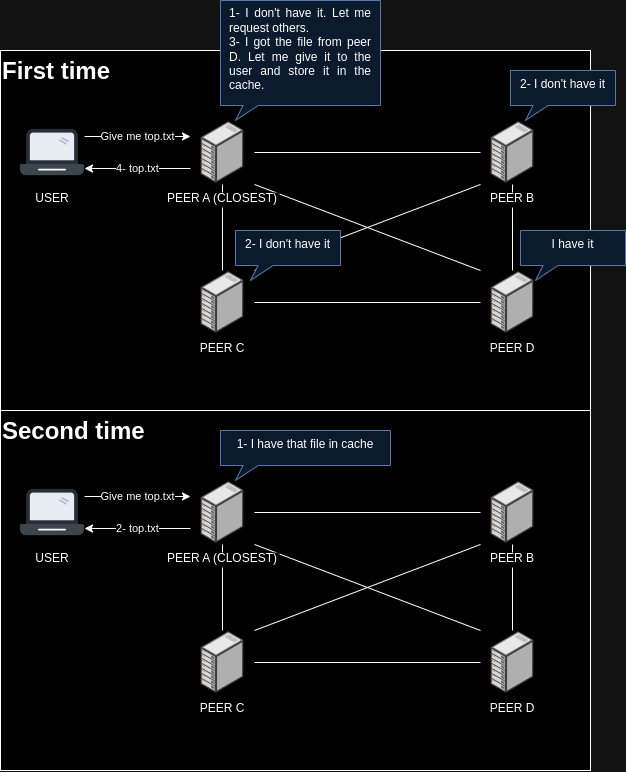
\includegraphics[width=0.5\textwidth]{assets/use-case-1/ipfs-behavior.drawio.png} % Change this to your image file
    \caption{Ipfs simplified}
    \label{fig:sample-image} 
\end{figure}

\paragraph{2º Phase: Study of ipfs composition}\mbox{}\\
In this phase, the time was spent almost around trying to understand concepts that were inherited from the \textbf{IPFS}. There were a lot of concepts, but a lot of them were focused on covering the \textbf{P2P} basics and how distributed systems started to have a body and a form. The main reason for calling this use case the starting building block for the second and future use cases to come is because the basics were all studied during this phase. However, a lot of general common knowledge about blockchains was gathered from public projects such as \textbf{Bitcoin} and \textbf{Ethereum} from an investor and technical curiosity perspective. With this in mind, in this section, there will be a basic overview of the main ideas from previous projects that were important for the conception of what is \textbf{IPFS} now.

\subparagraph{Kademlia DHTS}\mbox{}\\
\textbf{Kademlia} \cite{kademlia} is one of the ideas where \textbf{IPFS} got inspired. This algorithm is a decentralized hash table where it stores information relative to the most nearby peers in the network. The value stored comes from generating a public key within a range of space keys that are related to a given region and hashing it right away to form a \textbf{peer ID}. When creating a new node, this peer will first connect to a bootstrap node, and apart from there, it will recursively find more and more nodes, updating always its nearby peers as the peer receives requests and serves them. This update is based on checking the \textbf{k-buckets} of each peer that is serving the request, having the knowledge of more peers, and thereby updating it's table faster without having to communicate with a bunch of peers individually. This distance is calculated using an \textbf{XOR} distance procedure, where the comparison between two binary strings is done, resulting in a binary string that contains more or less 0's depending on its similarities. Every single position of a given peer ID binary string representation is compared with the same position of the other peer ID, resulting in 0 in case both positions are equal and 1 in case both positions are different. Such that in case the binary string representation has a lot of 0's, it means that the id is very alike; otherwise, it's very different, and because these id's are based in space ranges, having more similarities means more proximity between two heterogeneous peers, making this a decisive factor to decide if the table of a given peer should be updated or not. In case it does, the following 2 behaviors may occur: The k-bucket is full, adding a new item because it has more similarities that a member of this list will drop the farthest one and add this new one; The k-bucket is not full; adding a new item because it has more similarities than a member of this list will simply add the new one; With this mechanism, there is a guarantee that the peer will try to grab a file from the nearest peer first, while by not having requests during a certain amount of time this peer will make a scan on its own to make sure that this hash table is still relevant. More ahead, there is a graphical representation of such behavior.

\begin{figure}[H]
    \centering
    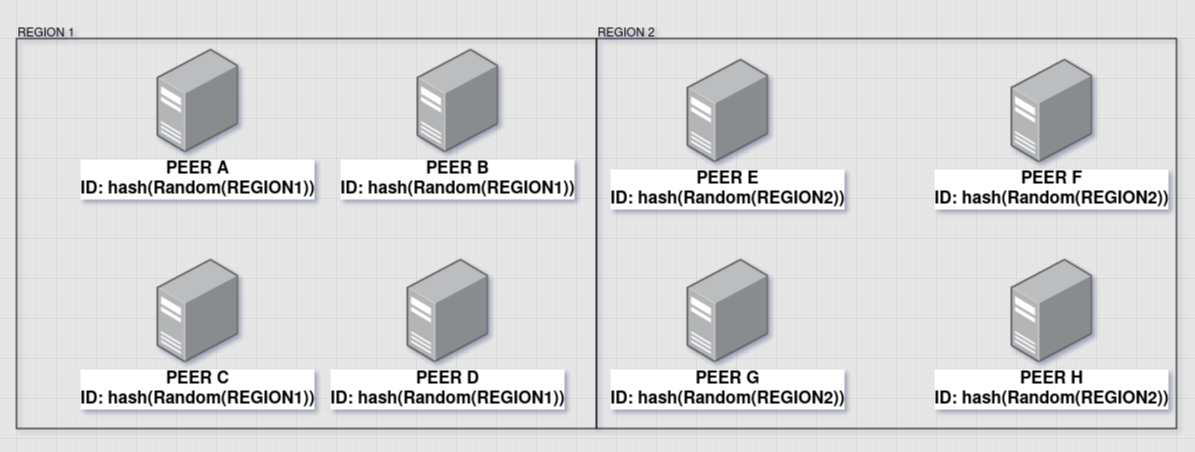
\includegraphics[width=0.5\textwidth]{assets/use-case-1/explain-kademlia.png} % Change this to your image file
    \caption{Kademlia: peer id generation}
    \label{fig:sample-image} 
\end{figure}

\begin{figure}[H]
    \centering
    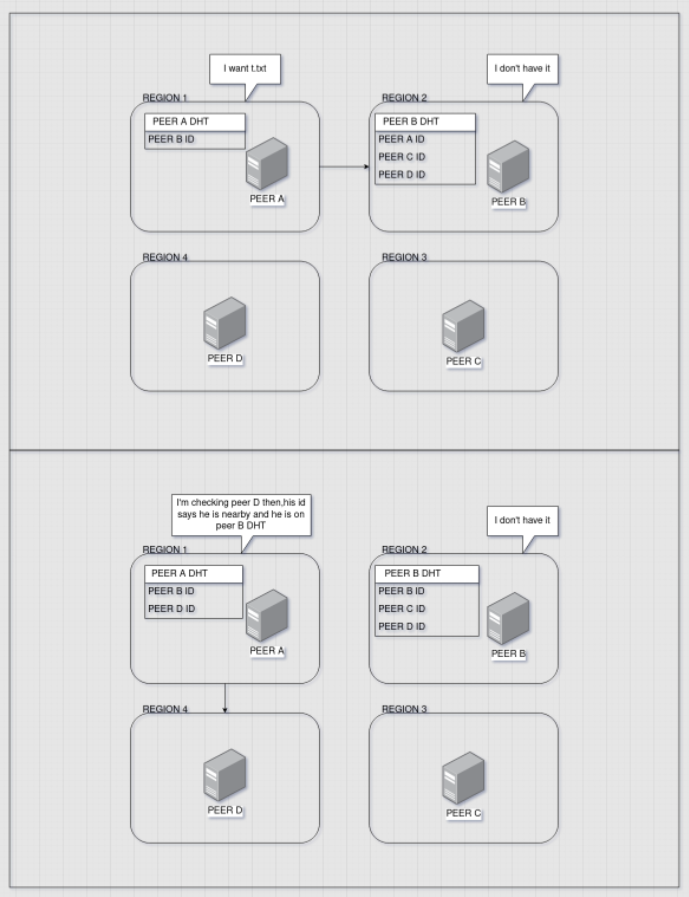
\includegraphics[width=0.5\textwidth]{assets/use-case-1/DHT.png} % Change this to your image file
    \caption{Kademlia: How it works for updating the k-buckets}
    \label{fig:sample-image} 
\end{figure}

\begin{figure}[H]
    \centering
    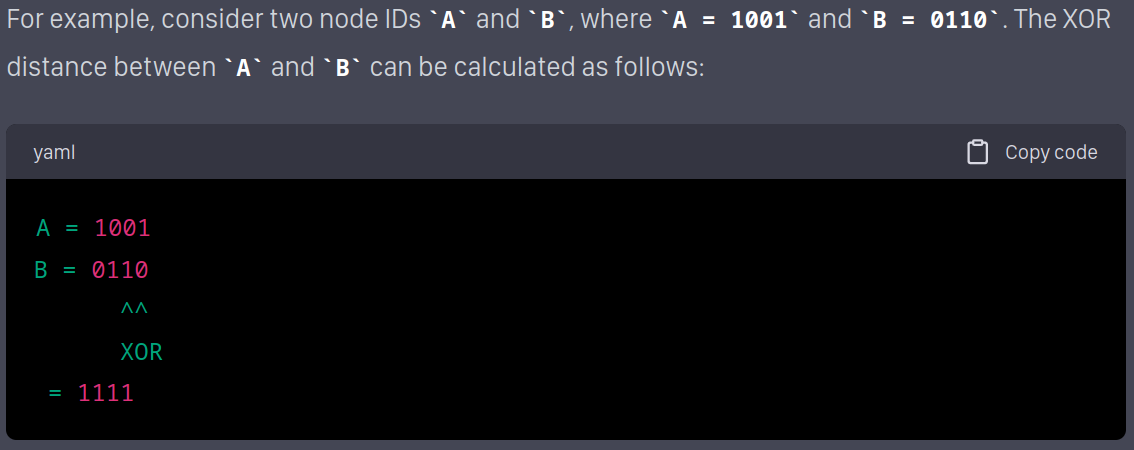
\includegraphics[width=0.5\textwidth]{assets/use-case-1/XOR1.png} % Change this to your image file
    \caption{Kademlia: Example 1 of XOR}
    \label{fig:sample-image} 
\end{figure}

\begin{figure}[H]
    \centering
    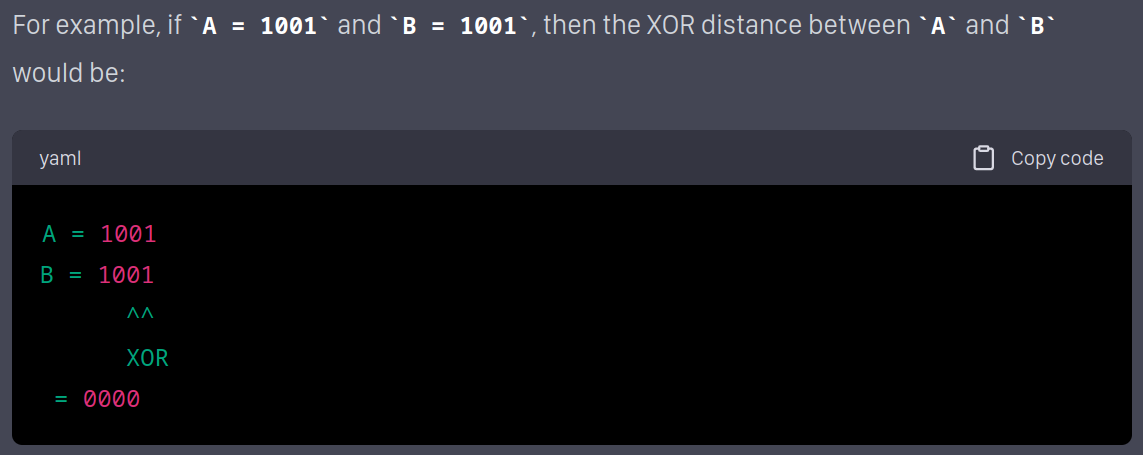
\includegraphics[width=0.5\textwidth]{assets/use-case-1/XOR2.png} % Change this to your image file
    \caption{Kademlia: Example 2 of XOR}
    \label{fig:sample-image} 
\end{figure}


\subparagraph{BitTorrent}\mbox{}\\
Another facet of \textbf{IPFS} is the way it shares blocks of data all over the network.
which was inspired in \textbf{BitTorrent} . \textbf{BitTorrent}, like \textbf{IPFS}, is a decentralized file system, though it does not call the data by an cid but instead the file name and
location. It is meant to provide scalability and efficacy in terms of downloading
files, because by storing the files in pieces, it makes it easier for a user to download
it faster. The big difference between the two is that IPFS is meant to long-term data storage and addressing content immutability, while the \textbf{BitTorrent} is more related to temporary data distribution \cite{bittorrent}.

\subparagraph{Git}\mbox{}\\
\textbf{Git} is another instrument where \textbf{IPFS} got some ideas. It provides a version control system that enables the user to go back in time and save some massive changes and update content. In order to do this it uses blobs, but instead of lists, it was trees; However, the concept is almost the same; the difference is that \textbf{IPFS} has an \textbf{Merkle DAG} and \textbf{Git} has a \textbf{DAG}. This data structure differs because \textbf{Merkle Dags} stores the hash of the hash, which means that it has the hash of the file as the hash of the children's.In contrast, the \textbf{DAG} only hashes the file itself. Which means that instead of retrieving the hash, you need the whole content, which in contrast in \textbf{Merkle dags} \cite{merkle-dag} you only need the hash of the children's, making the verification of hashes faster and still reliable. Also, \textbf{Git} is built in Ruby script and IPFs is built in Golang \cite{git}.

\subparagraph{SFS - Self Certified File System}\mbox{}\\
This is an extension of protocol that is aimed at security and creating secure channels. Ipfs has his own implementation, but the way they are represented is alike.
\textbf{Sfs} uses /sfs/<Location>:<HostID>, where the location is the server address and HostID = hash(publickey || Location). This way you can verify the peer while using the address because it was the location associated with the hash
plus the public key. In contrast, \textbf{IPFS} uses /ipfs/<CID> \cite{SFS}.

\subparagraph{Identities}  \mbox{} \\
This protocol refers to how \textbf{IPFs} identify their peers. This identification is executed like Kandemlia. An user can create a new peer ID whenever he wants to. Though it is recommendable that it stays the same, but users are free to
change it periodically if they feel to for questions of security. While connecting, the peers verify if the public key hashed corresponds to the peer ID; otherwise
The connection is rejected.

\subparagraph{Network}  \mbox{} \\
\textbf{Ipfs} can use any transport protocol, though the best suits are \textbf{WebRTC} and \textbf{uTP} or \textbf{SCTP}. Also, it uses \textbf{ICE NAT} transversal techniques; it checks the integrity of
messages using hash checksum and checks authenticity of messages using HMAC with senders public key. To know which protocol of transport we are using, IPFS needs to receive a multiaddress, which comes with the protocols used and
the way they are connecting \cite{webrtc} \cite{utp} \cite{sctp} \cite{ietf-ice}.

\begin{figure}[H]
    \centering
    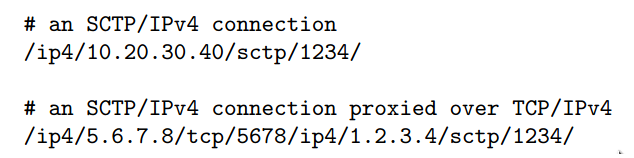
\includegraphics[width=0.5\textwidth]{assets/use-case-1/exampleNet+.png} % Change this to your image file
    \caption{IPFS: Example of multiaddress}
    \label{fig:sample-image} 
\end{figure}

\subparagraph{Routing}  \mbox{} \\
In terms of routing, preoccupations can be spotted perfectly when speaking about Kademlia. Despite based on it, Ipfs uses their methodology in sum with \textbf{coral} in their implementation. According to their white paper, there's an interface to deal with this tech, and the routing can be swapped if precautions are considered to fit their rules to that referenced interface.

\subparagraph{Blocks Exchange} \mbox{} \\
When discussing the way blocks are exchanged in \textbf{IPFS}, it must be put into conscience that it is very based on the BitTorrent protocol. However, the main difference relies on the way the object is retrieved. \textbf{IPFS} uses the \textbf{BitSwap} protocol, which is their own implementation for managing the transfer of blocks between peers. Both protocols are similar in the sense that both involve exchanging pieces of data (blocks) between peers, but \textbf{Bitswap} does not impose strict limits on the number of blocks a peer can request or provide, making \textbf{IPFS} more flexible in terms of the amount or type of data passed. Also, both implement a marketplace, whereas \textbf{Bitswap} can request any kind of block of data that it requires without this being necessary for the original request, function this way in a supply and demand paradigm, making this exchange more dynamic and flexible system when compared to \textbf{BitTorrent's} straightforward block exchange. Additionally, \textbf{Bitswap} implements a credit system called \textbf{Bitswap Credit}, which incentives peers to contribute to the network by either storing and providing data or searching and finding data for other peers. Thus, even if a peer doesn't have requested data blocks, it can still help the network. A \textbf{balancing contributions and block sharing} system is also implemented. This is because the network expects that every component delivers value to the network, and in case it does not, other peers may not prioritize serving the requests of the giving peer. Besides this, there are other mechanisms that help on that, like the sharing of blocks of peers with high demand with peers with small demand, making a "bigger fish" share its blocks with a "smaller" one, preventing "free-riders," and promoting the collaboration between all peers within the network environment \cite{bitswap}.

\subparagraph{Naming}  \mbox{} \\
Naming refers to the \textbf{IPNS} concept of \textbf{IPFS}. This is a \textbf{Interplanetary Naming System}, which can be used to create a point to \textbf{CID's}. This is very useful in situations where there can be multiple versions and there is the need to point to the most recent, which can be changed as there are new releases \cite{ipns}.

\subparagraph{Objects}  \mbox{} \\
In respect to the handling of objects within \textbf{IPFS}, it is well known that it got inspired on \textbf{Git}. This is because the objects have their value represented by hashes using a \textbf{Merkle DAG}. This represents a tree, which creates a deep linking between multiple objects that share a given relationship. As an example, in the event of having a directory, the behavior of storing such structure is to recursively hash the children's all together until having a single father, which represents the directory that owns all of the files. This system proves to be useful because not only does it provide content addressing, tamper resistance, and non-deduplication (file stored twice), but it also makes life easier when it comes to assertions since every file can be asserted against the tree with little few comparisons due to only having to hash the children's to prove that the file that is supposed to be the father is the actual father. In addition, this resulting hash is the before spoken \textbf{CID}, which is an ID that a user can use to identify which file is desired, while the person in charge still has the capability to create a given endpoint that controls the versioning like mentioned before. However, the user, by maintaining this \textbf{CID}, is known for a fact that the file he wishes is the same file ever.

\subparagraph{Files}  \mbox{} \\
To manage the merkle dag, there are multiple different data structures that can be used in \textbf{IPFS}, which are very alike \textbf{Git}: \textbf{Blobs},\textbf{List},\textbf{Trees} and \textbf{Commits}. 

Firstly, a blob is what it is used to actually store the data of the file, while having no links inside of it since it is supposed to be an actual file and not a directory.

\begin{figure}[H]
    \centering
    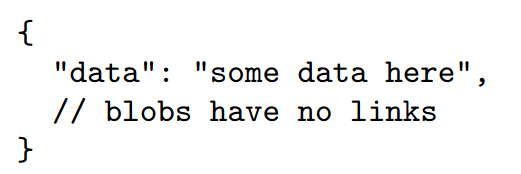
\includegraphics[width=0.5\textwidth]{assets/use-case-1/blobs.png} % Change this to your image file
    \caption{IPFS: blobs}
    \label{fig:sample-image} 
\end{figure}

Secondly, there is List which can have blobs and links inside, forming this way a array of objects that can either retain data or point to something that may contain data.

\begin{figure}[H]
    \centering
    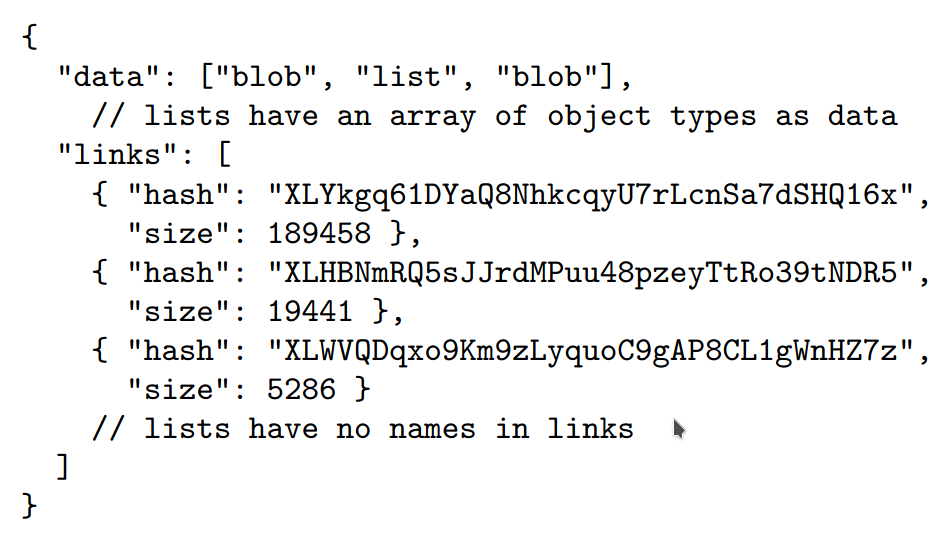
\includegraphics[width=0.5\textwidth]{assets/use-case-1/List.png} % Change this to your image file
    \caption{IPFS: lists}
    \label{fig:sample-image} 
\end{figure}


Thirdly, there is the tree which is the same thing as the list but the main difference is that it also contains name of files and can contain commits.

\begin{figure}[H]
    \centering
    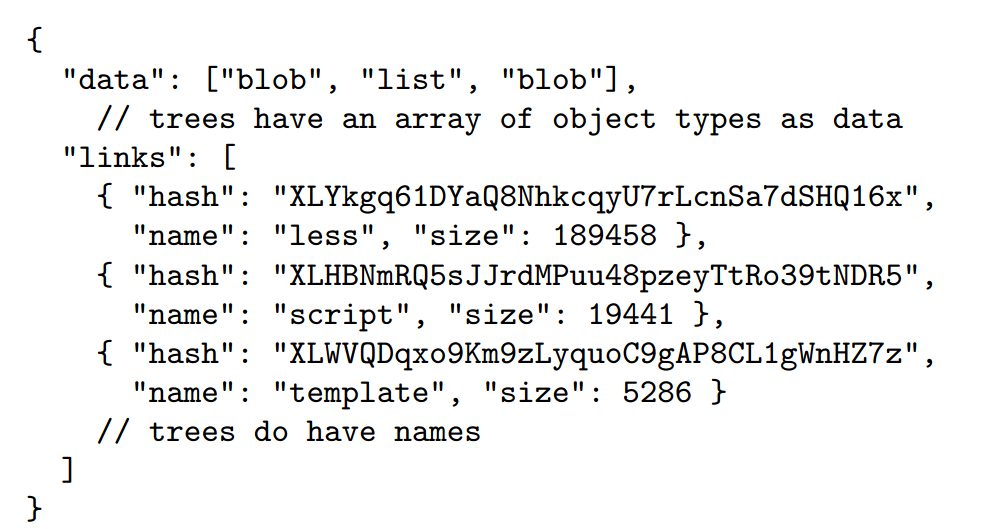
\includegraphics[width=0.5\textwidth]{assets/use-case-1/Trees.png} % Change this to your image file
    \caption{IPFS: tree}
    \label{fig:sample-image} 
\end{figure}


Lastly, there is the commit which represents a snapshot in the version history, representing changes that were made in a given file. In addition, it also links the author to the objects.

\begin{figure}[H]
    \centering
    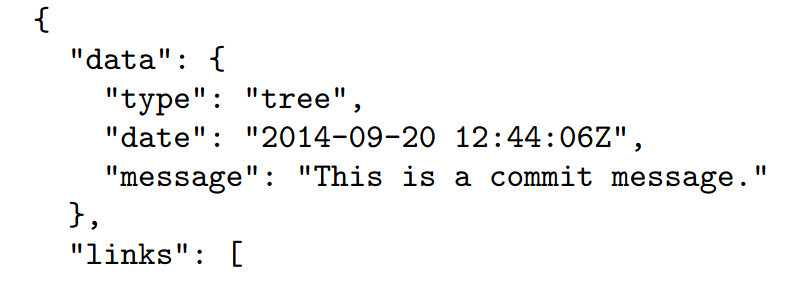
\includegraphics[width=0.5\textwidth]{assets/use-case-1/commit.png} % Change this to your image file
    \caption{IPFS: commit}
    \label{fig:sample-image} 
\end{figure}


\paragraph{3º Phase: Practical Implementation}\mbox{}\\
Reaching the third phase, after reviewing everything relative to \textbf{IPFS} and it's origin, a practical project was conceded just for creating a tangible way to obtain knowledge. This is important because relying only in documentation sometimes leaves some subjective understanding, which could result in bad insights. With comprehensive basic projects, there is more probability for this to not be the case. However, despite having practical insights this cannot be considered within the \textbf{DSR} methodology, precisely because there is no objective such as solving a real problem in sight.

The project was a decentralized per peer dropbox, which could be private or public depending of if you open the gateway to other peers or not. With such application, adding files on drop, add files from other peers using their \textbf{CID}, display the name of those files and it's information, download those files to our local machine, list all the connected peers and force an connection to an certain peer directly is possible. Pinning is not discussed, but it's something that could be done.

\begin{figure}[H]
    \centering
    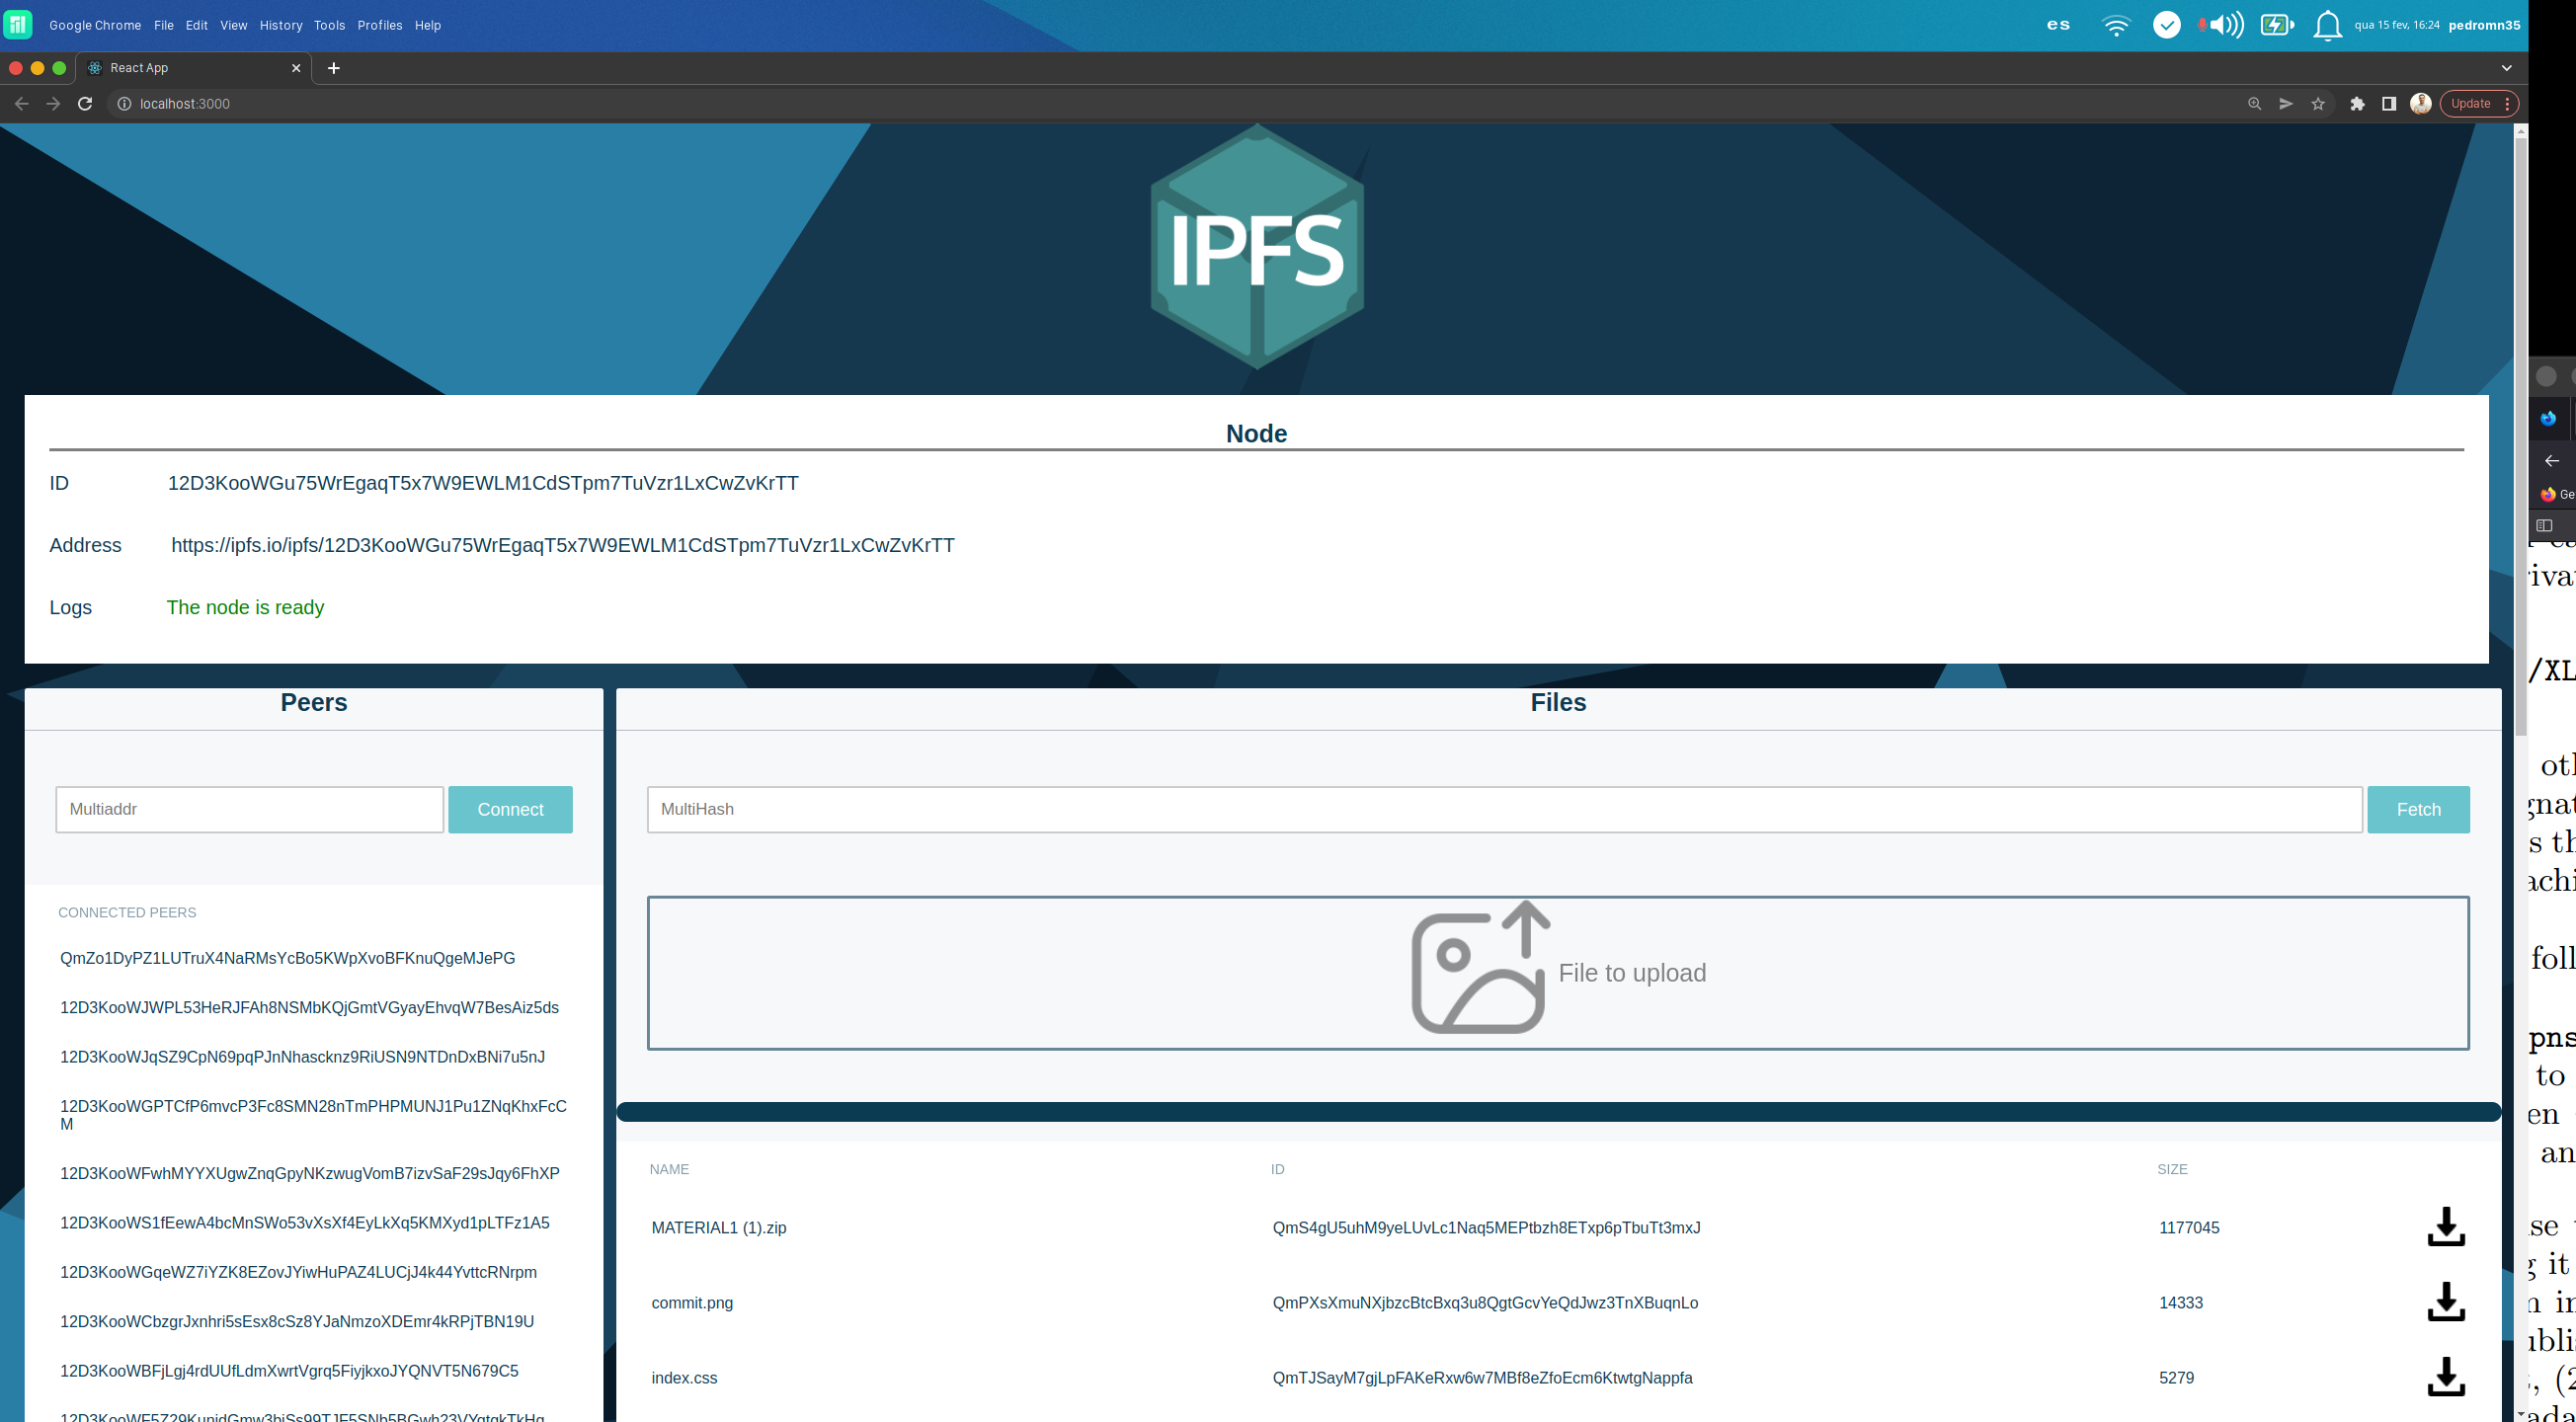
\includegraphics[width=0.5\textwidth]{assets/use-case-1/ipfshow.png} % Change this to your image file
    \caption{IPFS: Practical Implementation}
    \label{fig:sample-image} 
\end{figure}

\paragraph{4º Phase: Create a article regarding this project}\mbox{}\\
At this phase, the creation of an article was in sight. The objective was to try to think of a possible real implementation that could leverage both \textbf{IPFS} and \textbf{hyperledger fabric}. These ideas were the genesis block for the second use case. However, the feasibility of such in terms of performance is not confirmed because no benchmarking or works were released based on this idea, which is something that is in mind in the future work in this section. In addition, all of this must be intended to be private, which is possible by isolating the gateways for the peers only to work with a restricted collection of peers by leveraging their buckets. The target of such implementation was the healthcare environment.

The idea was simple but at the same time very intriguing. This is because the idea was to create a centralized point for managing nodes of each instance, while at the same time not enabling this person to actually mess with the data that is stored in each node. This is possible if strict policies are created in order to allow an admin to boot new instances and remove them from the stack. However, there must be rules that don't allow this single point of failure to change configurations or change sensitive data that will be present in each volume that an instance will be targeting. To achieve this, a layer diagram was constructed with the basic components that will be present in each node within an organization or different organizations. The way the cryptographic materials that identify each instance of the \textbf{hyperledger fabric} network will be disposed of depends on the setup that the organization wants. This requires a lot of thinking because nodes having the same origin of certificates or not could influence a lot how decisions are taken within the network, but since this is a theoretical conception, such considerations were not taken into account, and every node will work like it is from a different organization.

\begin{figure}[H]
    \centering
    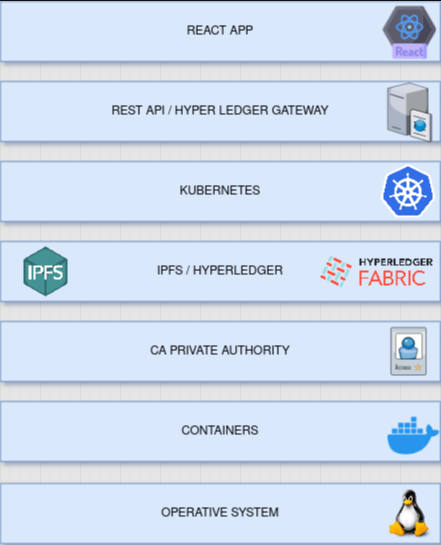
\includegraphics[width=0.5\textwidth]{assets/use-case-1/Layer.png} % Change this to your image file
    \caption{First use case: Layer Architecture}
    \label{fig:sample-image} 
\end{figure}

Besides the layer representation, schemas around how these components would be placed in each node were also done where this network would be built around a \textbf{Kubernetes} cluster and the disposition of resources would be the same among nodes, though supposedly it's not recommended that the master node has the same number of components that others have. The number of peers is variable, and there is only one instance of an \textbf{IFPS} node per node, but that's something that depends on the admin to decide. This is just a conception demonstration; the way things are done in the second use case is completely different because a lot of other aspects were considered, like the size of the network and the resources that the organization may have. Also, a simple example of a network was created where multiple peers inside of a given node are apart of different channels. In the provided schema, a peer of type admin could access both channel admin and group channel, where a peer destined to be apart of a group channel is only apart of the group channel. It should be kept in mind that when a peer is apart of 2 channels, it will have a ledger for each, but that's something that was not illustrated to simplify the diagram. Also, having more than one peer per node is something that should be thought through well because each peer instance is very powerful, and in this representation, the idea was to have a single node for the orderers. Additionally, there could be multiple types of networks with different channels and permissions, but like I mentioned before, this was just a very simple example of the network capabilities. A possible interaction of a doctor with the network was also conceded.

\begin{figure}[H]
    \centering
    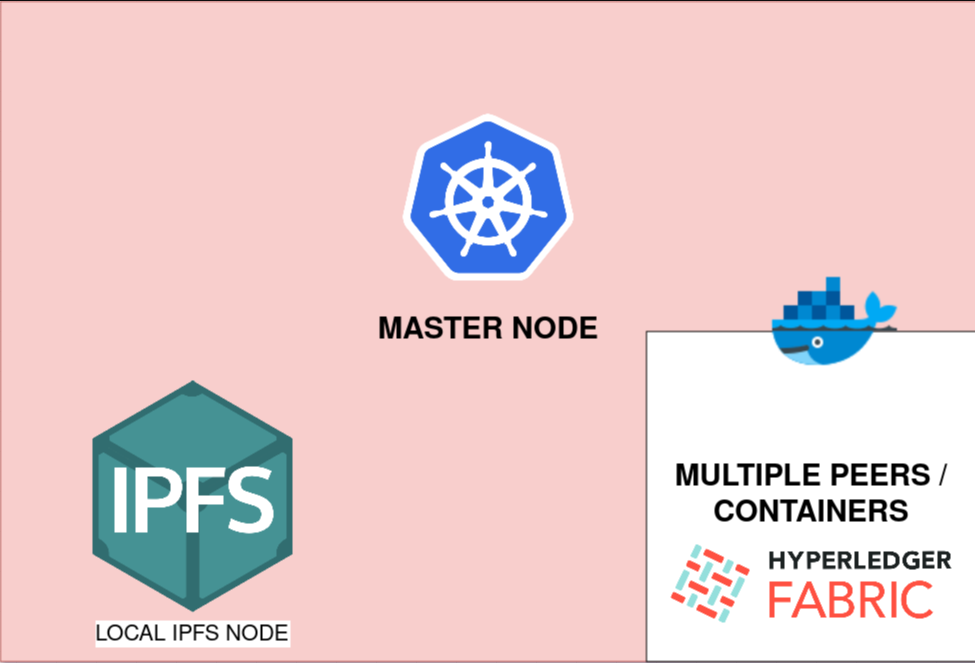
\includegraphics[width=0.5\textwidth]{assets/use-case-1/Master.png} % Change this to your image file
    \caption{First use case: Master node composition}
    \label{fig:sample-image} 
\end{figure}

\begin{figure}[H]
    \centering
    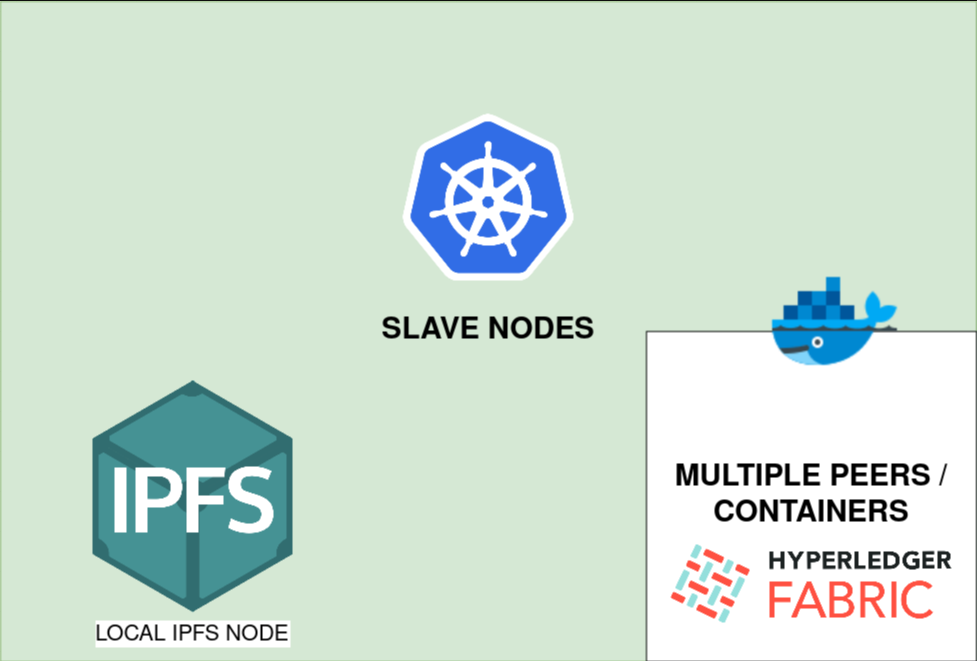
\includegraphics[width=0.5\textwidth]{assets/use-case-1/Slave.png} % Change this to your image file
    \caption{First use case: Slave node composition}
    \label{fig:sample-image} 
\end{figure}

\begin{figure}[H]
    \centering
    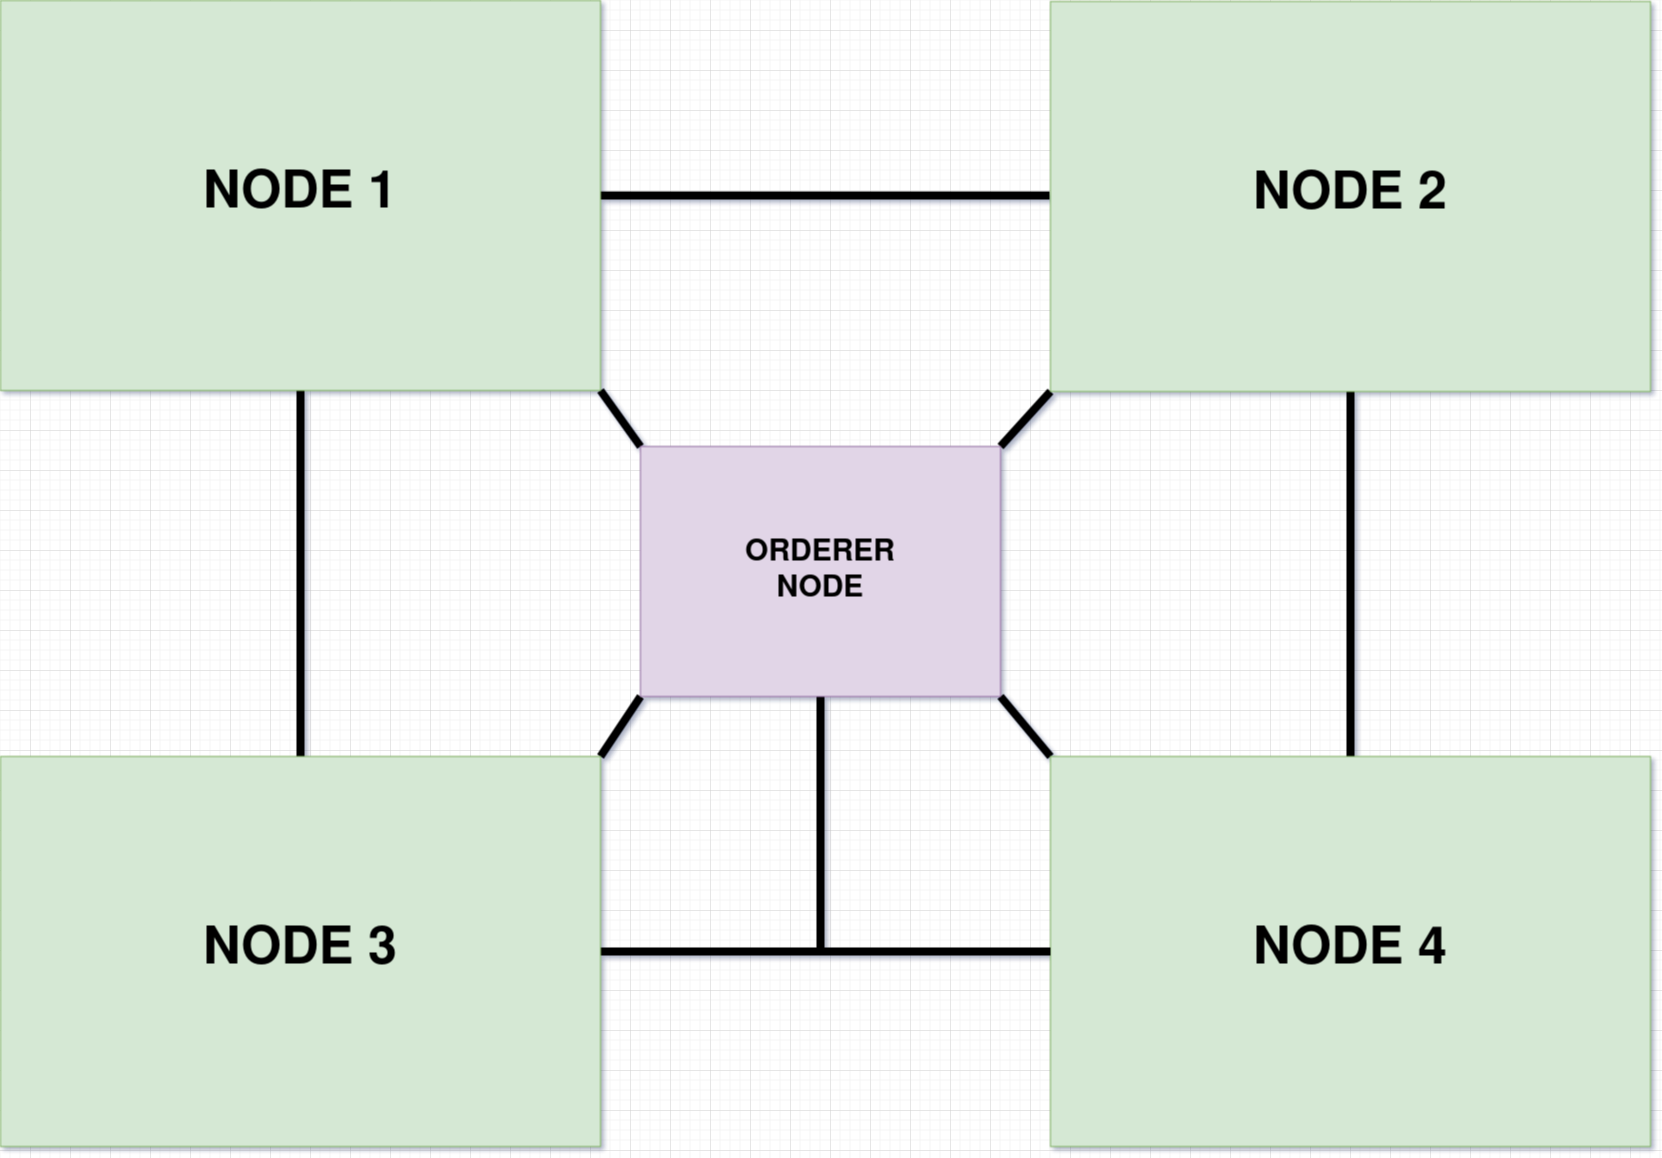
\includegraphics[width=0.5\textwidth]{assets/use-case-1/global-vision.drawio.png} % Change this to your image file
    \caption{First use case: Global vision}
    \label{fig:sample-image} 
\end{figure}

\begin{figure}[H]
    \centering
    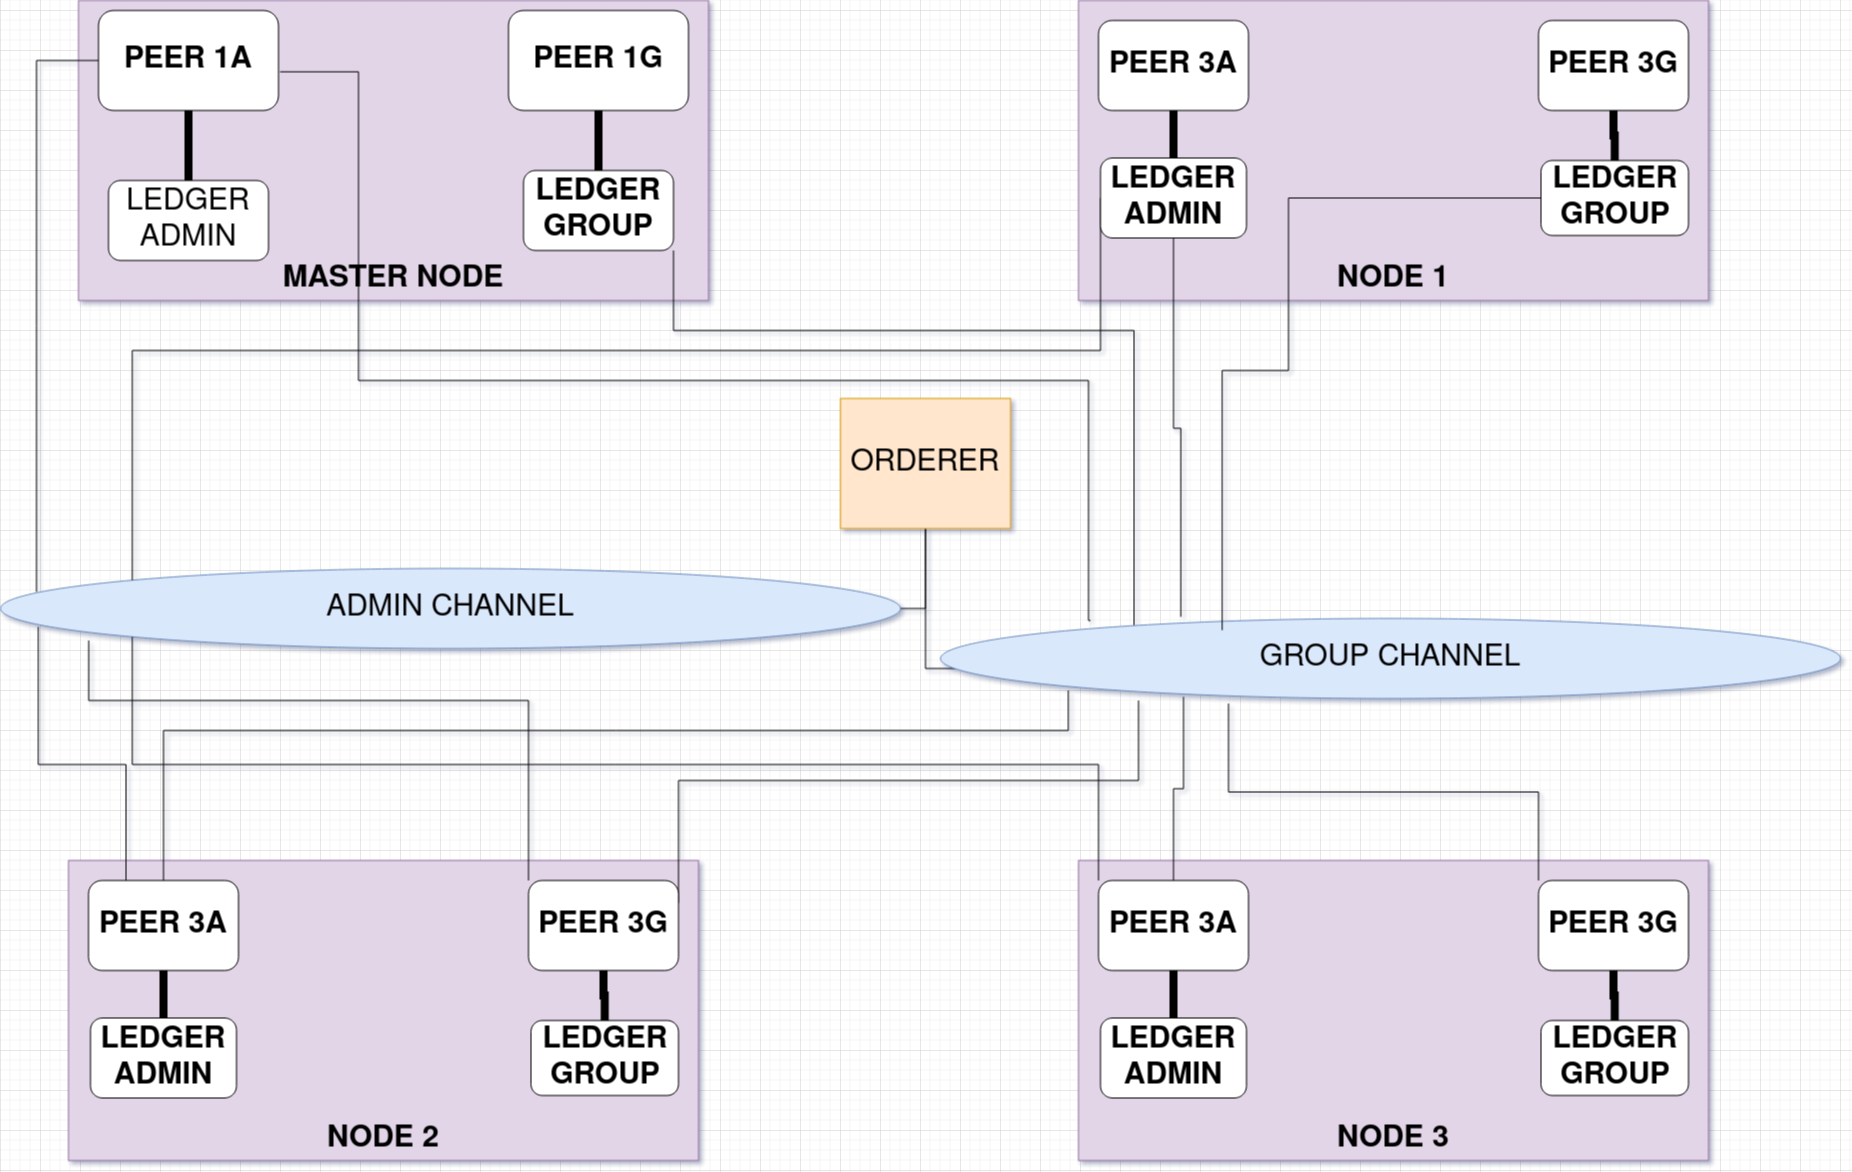
\includegraphics[width=0.5\textwidth]{assets/use-case-1/hyper-ledger-view.drawio.png} % Change this to your image file
    \caption{First use case: hyperledger fabric simple network example}
    \label{fig:sample-image} 
\end{figure}

\begin{figure}[H]
    \centering
    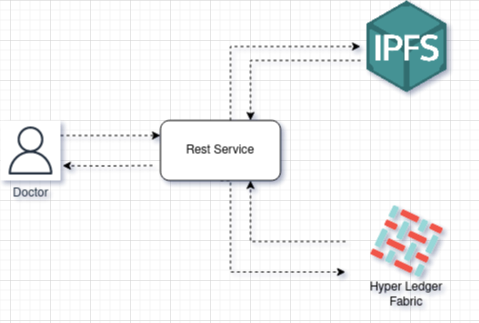
\includegraphics[width=0.5\textwidth]{assets/use-case-1/workflow.png} % Change this to your image file
    \caption{First use case: Workflow}
    \label{fig:sample-image} 
\end{figure}


\paragraph{5º Phase: Review the article regarding this project}\mbox{}\\
In this phase a deep review to the article was done, corrections were taken and after everything appeared well the article was successfully accepted for the conference.

\paragraph{6º Phase: Present the Article}\mbox{}\\
Within the final phase, the article was presented in the blockchain congress, giving more insights of what is being implemented currently in the private landscapes, contributing to more interesting ideas regarding future work around this matter. 

\begin{longtable}{|c|c|c|c|c|}
    \hline
    & \textbf{April}& \textbf{May} & \textbf{June} & \textbf{July}  \\ \hline

    \textbf{1º Phase: Ipfs deep dive}  & X & & & \\ \hline

    \textbf{2º Phase: Study of Ipfs composition} & X & X & & \\ \hline

    \textbf{3º Phase: Practical Implementation} & & X & X & \\ \hline

    \textbf{4º Phase: Create a article regarding this project} & & X & X &  \\ \hline

    \textbf{5º Phase: Review the article regarding this project} & & & & X \\ \hline

    \textbf{6º Phase: Present the Article} & & & & X \\ \hline
    
    \caption{Monthly plan 2023: Ipfs use case} \label{tab:activity_schedule} 
\end{longtable}

\subsection{Approach}
Relatively to the approach that was taken during this part of the work, like specified before, the \textbf{DSR} was not followed due to the fact that practical creations in the direction of solving a problem were not inferred, leaving as the only valid path to investigate, doing some theoretical conceptions around the subject and thinking after how this could actually be put into practice, which was the main reason why the second use case occurred. In other terms, no framework was adopted, but a lot of insights were taken by own procedures.

\subsubsection{Discussion}
As discussion, there will be the presence of a  reflection about the bad sides and positives sides of the given project. In that behalf, \textbf{SWOT}(Strengths,Weaknesses, Opportu-
nities, Threats) diagram was created:

\begin{figure}[H]
    \centering
    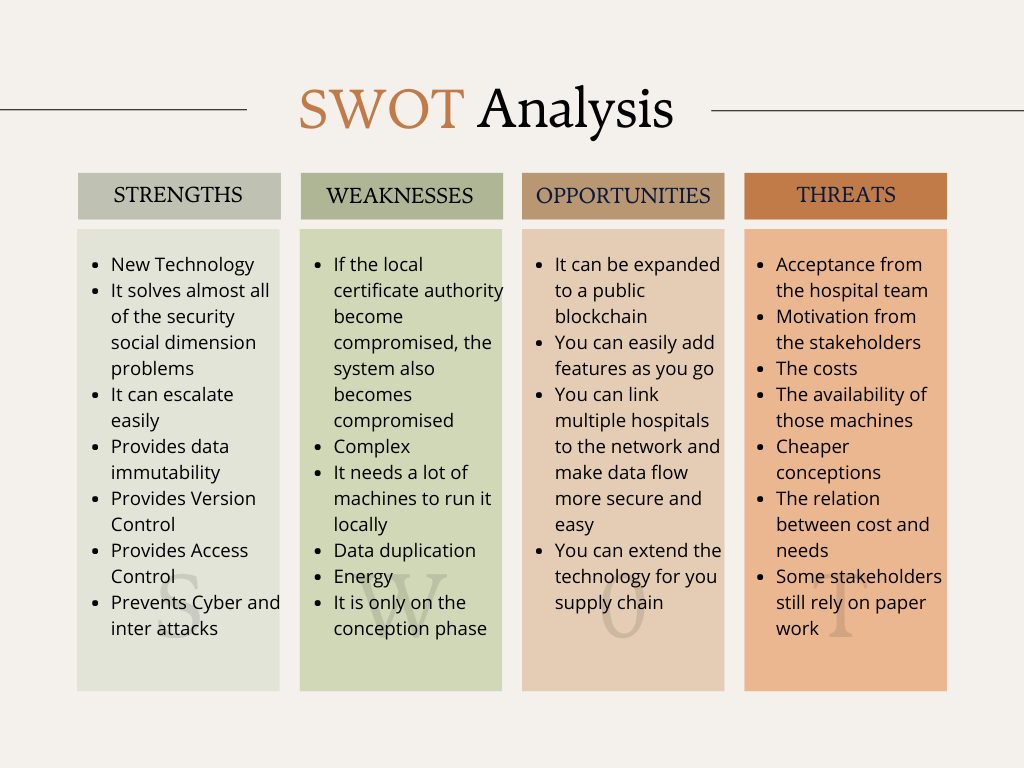
\includegraphics[width=0.5\textwidth]{assets/use-case-1/swot.png} % Change this to your image file
    \caption{First use case: Swot}
    \label{fig:sample-image} 
\end{figure}

\subsubsection{Conclusion} 
In conclusion, despite not being implemented, this project seems to have a lot of work and possibilities, and it will be very interesting to see until each measure such a random idea could play out. It's feasibility is still something unknown, but constructing things and applying them into practice is one of the fundamental needs of engineering, and since this project works with 2 different approaches for data immutability, the healthcare environment could benefit in terms of security and traceability like it never did, which could potentially revolutionize the methodologies used to work with data within the healthcare landscape, but further research and work is still required to understand how this can impact it, making it something truly nutritional for emergent technology enthusiasts.

\subsubsection{Future Work}
This project works as an extension of the second use case, even though it was the one that originated it. The work is being conducted all around this project, and the future work will be conducted around the same idea, which is solving component by component of the previously shown architecture. Hyperledger fabric has been solved with the last work, and what is expected next is to do something alike that experience but now with \textbf{IPFS}. Also, possible improvements will be expected in delving into this, but that is something that will be better covered in this section. The expected work items for the future are the following:

\paragraph{Creation of a private IPFS network} \mbox{} \\
One of the work items to be expected is the creation of a private \textbf{IPFS} network. This is because the \textbf{Hyperledger fabric} has been uncovered already in the second use case, making it necessary, like said before, to uncover the remaining components, more concretely the \textbf{IPFS}, private network.

\paragraph{Benchmarking of the IPFS private network} \mbox{} \\
Another work item would be to benchmark the \textbf{IPFS} private network to actually understand until each measure is efficient in private environments. In case it is not, maybe it would not be that clever to keep going with this idea, but it is still interesting to give insights of the following steps in case it does not come to be a fail.

\paragraph{Creation of a hyperledger fabric network that was IPFS as it's extension} \mbox{} \\
In case the benchmarking over the private network goes right, there is also the intension of creating a conjunction of both \textbf{IPFS} and \textbf{Hyperledger fabric}, which was the actual main objective at first glance of the idea.

\paragraph{Benchmarking of the network that implements both IPFS and hyperledger fabric} \mbox{} \\
In the realm of testing the feasibility of mixing such 2 powerful components, there is the benchmarking of the later mentioned network which could lead to a continuation or banishment of the idea in cause.

\paragraph{Creation of a web client} \mbox{} \\
The most important component when it comes to this kind of implementation is the way users will interact with it. A client that is capable of both storing files and simply sending transactions will be needed.

\subsection{Hyperledger Fabric: Seeking standardization through designing for each type of organization}

In the advent of the second use case, it should be known that it is concerned about having the best infrastructure that could be implemented within a healthcare institution. Here, by recurring to a \textbf{DSR} methodology, there is the gathering of both theoretical and practical knowledge about such. Requirements are reunited, networks with different typologies, sizes, concepts and benchmarkings, there is comparison between solutions, and conclusions regarding this work are present with a given provence of success. Putting in another perspective, this is the network infrastructure that would be required in the first use case, which is the main reason why the first is associated as an extension. In this section, it is expected to present \textbf{Objectives},followed \textbf{plan},\textbf{approach},\textbf{implementations},\textbf{compare solutions},\textbf{final architecture},\textbf{discussion},\textbf{future work} and \textbf{conclusion}, but this will be better covered as it moves forward.

\subsubsection{Objectives}
When speaking about the objectives in this use case, the main one is to answer the research question, "What kind of infrastructure design is necessary to support a blockchain solution in such a vast and complex environment as healthcare?". This question will be answered by creating means to an administrator becoming capable of managing a blockchain network using a single point of failure. This is necessary because having multiple nodes within our organization makes it not feasible to configure due to the fact that it would require connecting to each node to make the necessary changes, which with these ideas could be something easier to setup. This requires sacrificing a bit of security over usability, but that is something that could be faced by using really good authentication mechanisms and also allowing the administrator to only be able to add or remove elements from the nodes without changing the data and configurations that each element may have. Additionally, the administrator should be capable of adding members with new configurations, but this is something that can be discussed further.

\subsubsection{Plan}
A plan is always something critical when it comes to keeping track. This enables both personal and also professional goal achievement, involving setting objectives, determining strategies, and organizing resources to reach desired outcomes.

In the general plan, there was a highlighting of all the activities and steps in a broad way. However, like in the first use case, there is the need to go even deeper within that plan and understand what was done more specifically to the second use case. With this in mind, a lot of what has been done so far will be covered in this section, explaining not only what was done during that period but also when it was done. Additionally, it is important to understand that most of the activities resulted from a \textbf{DSR} perspective where this solution has been evolving smoothly.

\paragraph{1º Phase: Gather requirements}\mbox{}\\
In the first instance, there was the gathering of requirements. This requirement could be of the typical two types: \textbf{functional} and \textbf{non-functional}.

\textbf{Functional} requirements are those that describe what a system should do, defining what behavior and specific functions a system should have. Those are usually derived from the user's needs and expectations and are essential for the software to perform as it is intended. As an example, there are things such as \textbf{user authentication}, \textbf{user authorization}, and \textbf{interaction with external systems or databases} \cite{functional-requirements}.

\textbf{Non-Functional} requirements, on the other hand, are the description of how the system should perform rather than what it should do. Those are the requirements that ensure that the system has quality and overall performance while covering aspects such as usability, reliability, performance and security. As an example, there could be mentioned in the performance sphere the system \textbf{responding to user requests within 2 seconds}. For scalability the need of a \textbf{system handling up to 1 million users} and for security \textbf{data being encrypted during transmission and storage} \cite{non-functional-requirements}.

For this project, since it is within a research realm, there were not many limitations in terms of requirements. In fact, those limitations were what was under research in some cases. However, in terms of \textbf{functional} requirements for admins (since the project is focused on the infrastructure), there were some set of requisites such as: \textbf{user authentication},\textbf{user authorization},\textbf{interaction with existing systems},\textbf{should provide an on-premise infrastructure},\textbf{the infrastructure should be easy to manage},\textbf{data must be exchanged securely},\textbf{the infrastructure should be easy to debug},\textbf{the infrastructure should be easy to observe},\textbf{the infrastructure should have a block explorer},\textbf{ the infrastructure should be scalable}, and \textbf{the infrastructure should be secure}. In addition, in terms of \textbf{non-functional} requirements, the ones that could be described at this point are: \textbf{usability should be user-friendly and accessible} and \textbf{there must be unauthorized access and integrity of data insurance}, rather than those that will be considered after the gathering of the benchmarkings to simply check if the system fits the needs of the organization.

\paragraph{2º Phase: Study the methodology framework}\mbox{}\\
Since the project's very complex, having a \textbf{methodology framework} is a must, essential for ensuring structured, consistent, and repeatable processes. With this in mind and like mentioned before, this project will be faced using \textbf{DSR} practices, which are crucial for seeking the bridge gap between theorical and practical applications. Studying this framework was the main objective in this phase.

\paragraph{3º Phase: Interim Report} \mbox{}\\
For the dissertation, an interim report was an obligation, which was something that had been developed along the way during this phase. Conceding this report is necessary because it was a way of responsible for analyzing, validating and approving the theme under research.

\paragraph{4º Phase: Reading all of hyperledger fabric and it's components theory}\mbox{}\\
This phase was one of the most important within the lifecycle of the project. Articles about hyperledger fabric and documentation were meticulously read, gaining a lot of knowledge that could be later used for the creation of the first network.

Relatively to the documentation, the most important sections were the ones within the \textbf{key concepts} such as the \textbf{hyperledger fabric model},\textbf{how fabric networks are structured},\textbf{identity},\textbf{MSP's},\textbf{policies},\textbf{peers},\textbf{ledgers},\textbf{ordering service},\textbf{smart contracts and chaincode},\textbf{fabric chaincode lifecycle},\textbf{private data} and \textbf{security model}. In addition, there was a following of operational practical guides around how to setup each of the components of the hyperledger fabric, like \textbf{Certificate Central Authorities},\textbf{peer},\textbf{orderer},\textbf{chaincode},\textbf{channel}, and \textbf{ledger}.

Within the \textbf{hyperledger fabric model}, there was a dive into the design of the framework, presenting the main concepts that are present that form the blockchain network, like the concepts of \textbf{asset},\textbf{chaincode},\textbf{ledger},\textbf{privacy},\textbf{security and membership services}, and the \textbf{consensus}.

\textbf{How fabric networks are structure} was another important topic because it explains how the blockchain is configured, taking as an example the \textbf{sample network} that they provide for practical insights, while showing in theoretical terms how to create the network, how certificate authorities operate, how nodes are joined into a channel, how the chaincode lifecycle operates, how to use the chaincode, how to join multiple components in multiple channels, how to create new channels, how to join components to the new channel, how to add an organization to an existing channel, and how to add existing components to newly joined channels.

\textbf {Identity}, another section of the key concepts, was a section to give important insights of how authentication is managed within the network. This was done through explaining the usage of an identity, X509 certificates, \textbf{PKI} (public key infrastructures), digital certificates, authentication, public keys, private keys, certificate authorities, root certificate central authorities, intermediate certificate central authorities, and \textbf{CRL} (certificate revocation lists).

After the identity section, the key features also provide more information about what exactly a \textbf{MSP} is, which is something that uses as its base the previous section: \textbf{MSP}'s leverage the concepts of identity to develop their activity, which is to prove identity to the rest of the network.

In the \textbf{policies} section, there is reference to the definition of what is a policy, why they are needed, how policies are implemented, how to write them in fabric, the chaincode lifecycle, and even how to override the policy definitions.

The \textbf{Peers} section exists for having a theoretical overview of the role of the peer within the \textbf{hyperledger fabric} network. Questions like the peer playing in chaincode terminology, ledgers, chaincode,transaction lifecycle, organizations, identity, and orderers are discussed.

When it comes to the \textbf{Ledger}, there can be introduced the concept of what is a ledger, what kinds of state there is in it, it's play in blockchain's, how does it come from transactions and blocks, it's database options, ledger namespaces, and ledger and channels.

On the \textbf{Ordering} section, there is everything that is needed to understand with respect to an orderer component: its configurations, its identity, the transaction flow, and consensus algorithms.

Another concept that it has is \textbf{Smart Contracts and Chaincode}, where there are theoretical assumptions about smart contracts, it's play in ledgers, what is endorsement, how transactions are validated, it's play in channels, the default channels that are always present in peers, and system chaincodes in more depth.

\textbf{Fabric Chaincode Lifecycle} is a section to define more in depth what a chaincode is and how to deploy, install, and upgrade.

To introduce the concept of \textbf{private data collections}, there is also the section \textbf{private data}. While introducing it, it also gives examples about how to work with it.

Finally, within the key concepts, there is also the section referring to the \textbf{security model}, mentioning how \textbf{hyperledger fabric} offers security within it's network and explaining extra capabilities. With relation to security identities, MSP's,Policies,Peers,orderers,TLS, and HSM (hardware security models) are mentioned components.

Moving to the practical guidelines, they were very helpful to construct a operational guide to boot a network from scratch which is important for later reference, since some configurations of \textbf{hyperledger} are more into the taste of the operator, thereby creating some fuzzy subjectiveness because concrete implementations were not presented and that was something that presented as a difficulty during the conception.  However, this guidelines despite being very complete and useful remain with needs of restructuring for better understanding. Everything is created in a github repository using markdown files.

The first guideline was around the \textbf{CA's}, describing how to setup a \textbf{hyperledger fabric} own certificate central authority like creating the CA,explaining it's components,configuring it,explaining how to revoke certificates,how to register new certificates, how to enroll certificates and explaining how to create a chain of certificate central authorities.

\begin{figure}[H]
    \centering
    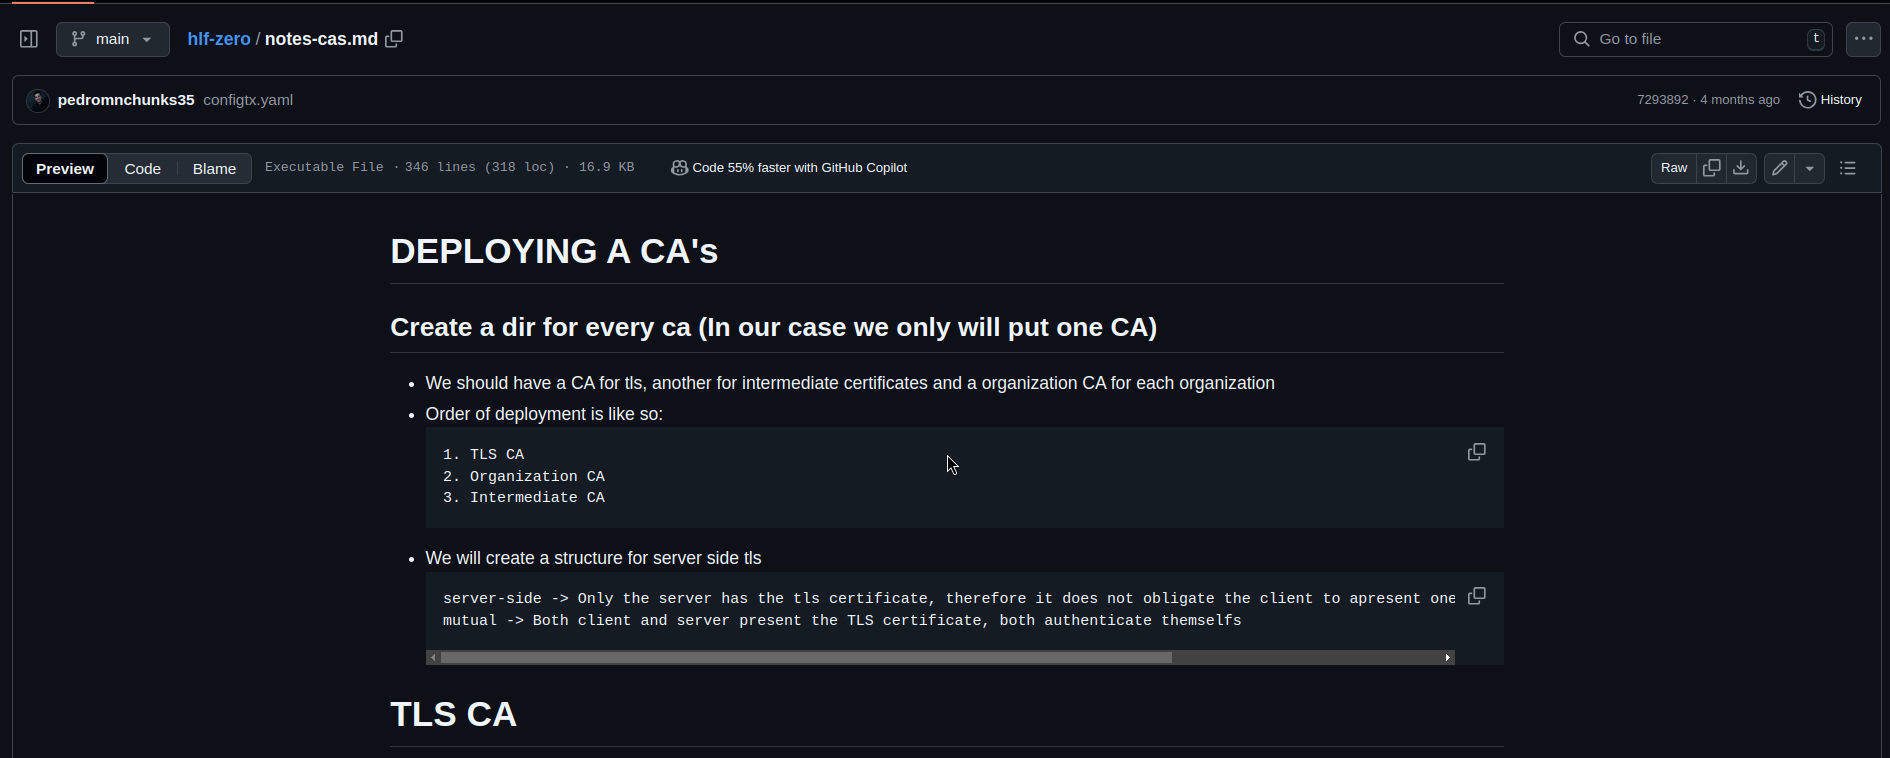
\includegraphics[width=0.5\textwidth]{assets/use-case-2/notes-cas.png} % Change this to your image file
    \caption{Second use case: ca's operational guide}
    \label{fig:sample-image} 
\end{figure}

The second guideline was more around the \textbf{orderers}, focused on introducing how to deploy a orderer. This is done by creating it's identities, creating a structure for the usage of each identity within the configuration file of the orderer and for later dependencies such as channel creation.

\begin{figure}[H]
    \centering
    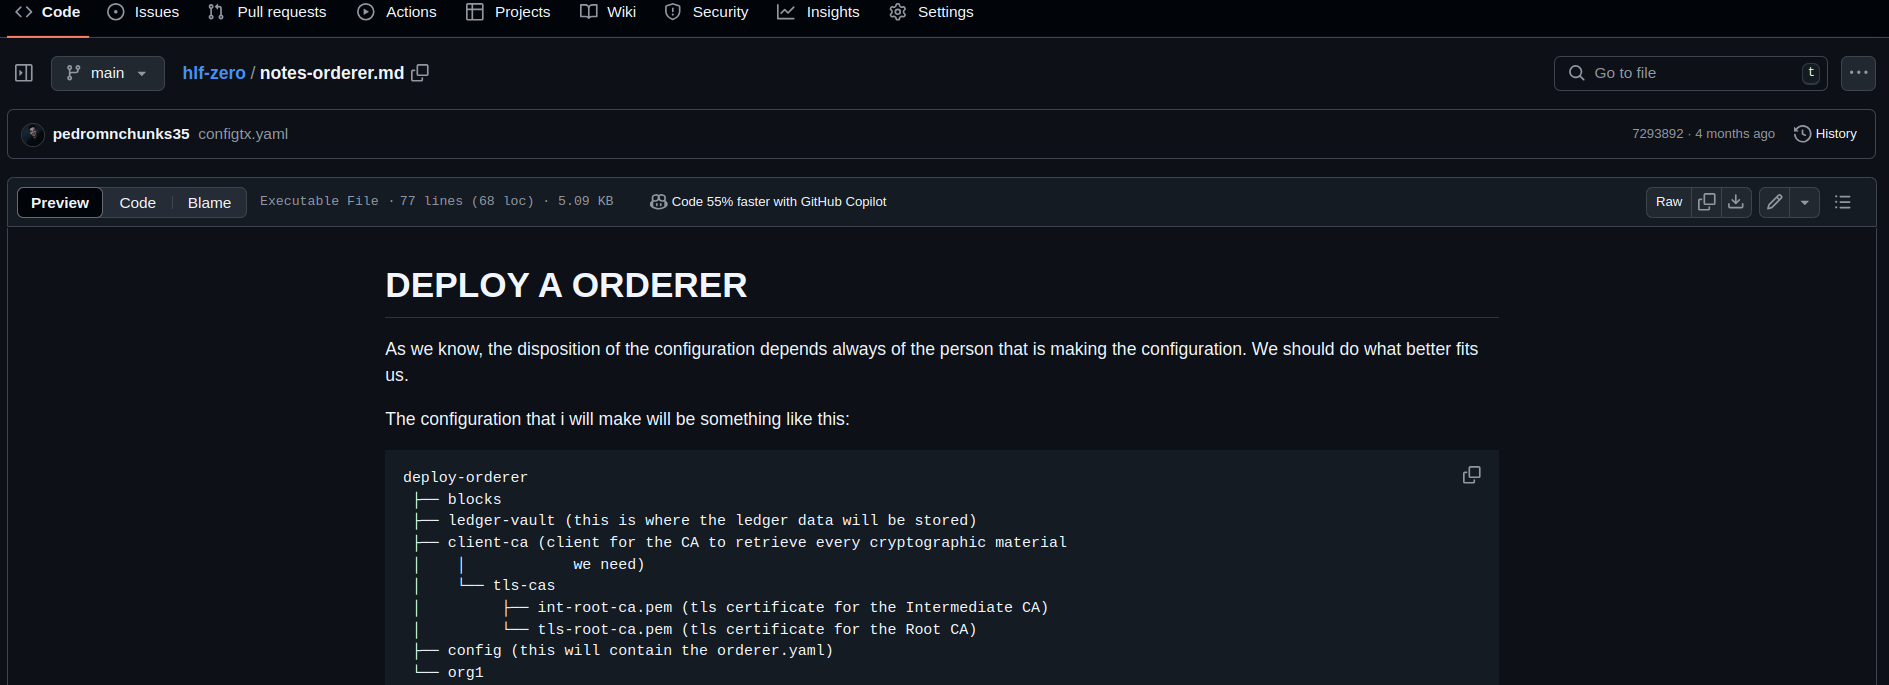
\includegraphics[width=0.5\textwidth]{assets/use-case-2/notes-orderer.png} % Change this to your image file
    \caption{Second use case: orderer operational guide}
    \label{fig:sample-image} 
\end{figure}

The third guideline was directed for the \textbf{ledger}, which despite having multiple options of databases to choose, the choosen one was actually the couchdb. This is because this ledger is currently the standard one. Also, it is important to mention that there was a need to start by the ledger because the peer requires the ledger as dependency to actually remain deployed, otherwise it will crash due to not having it.

\begin{figure}[H]
    \centering
    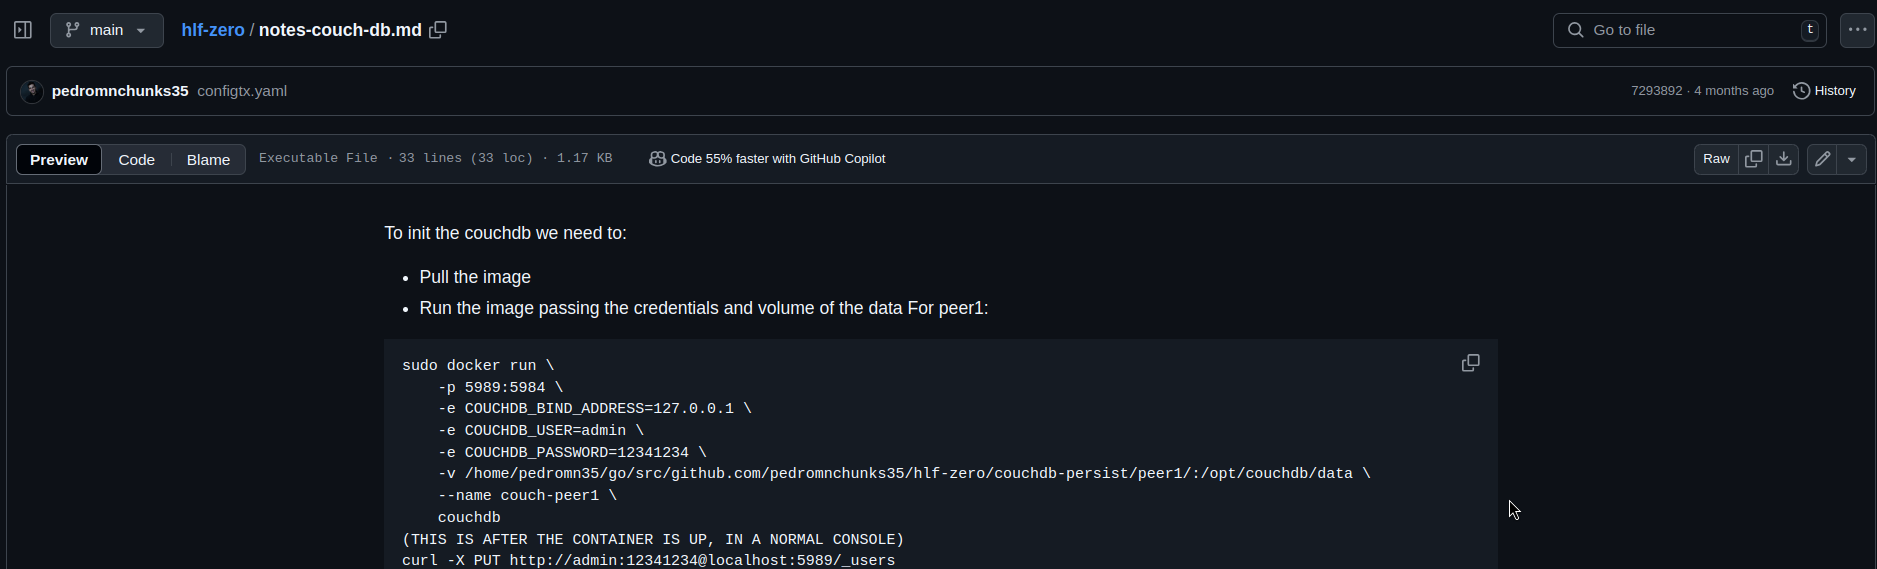
\includegraphics[width=0.5\textwidth]{assets/use-case-2/notes-couch.png} % Change this to your image file
    \caption{Second use case: couchdb operational guide}
    \label{fig:sample-image} 
\end{figure}

Moving to the forth, this time the \textbf{peer} took precedence, which is normal since the last tutorial was it's dependency. Alike in the orderer, the focus was to create it's identities,structure and configuration. Both orderer and peer were deployed in debug mode for having more info about why something was not working at that time. This was crucial because, like mentioned before most of the operational guides had some subjectiveness in the structure: this disposition of the configurations was a bit at the taste of the operator in question under creation of deployment.

\begin{figure}[H]
    \centering
    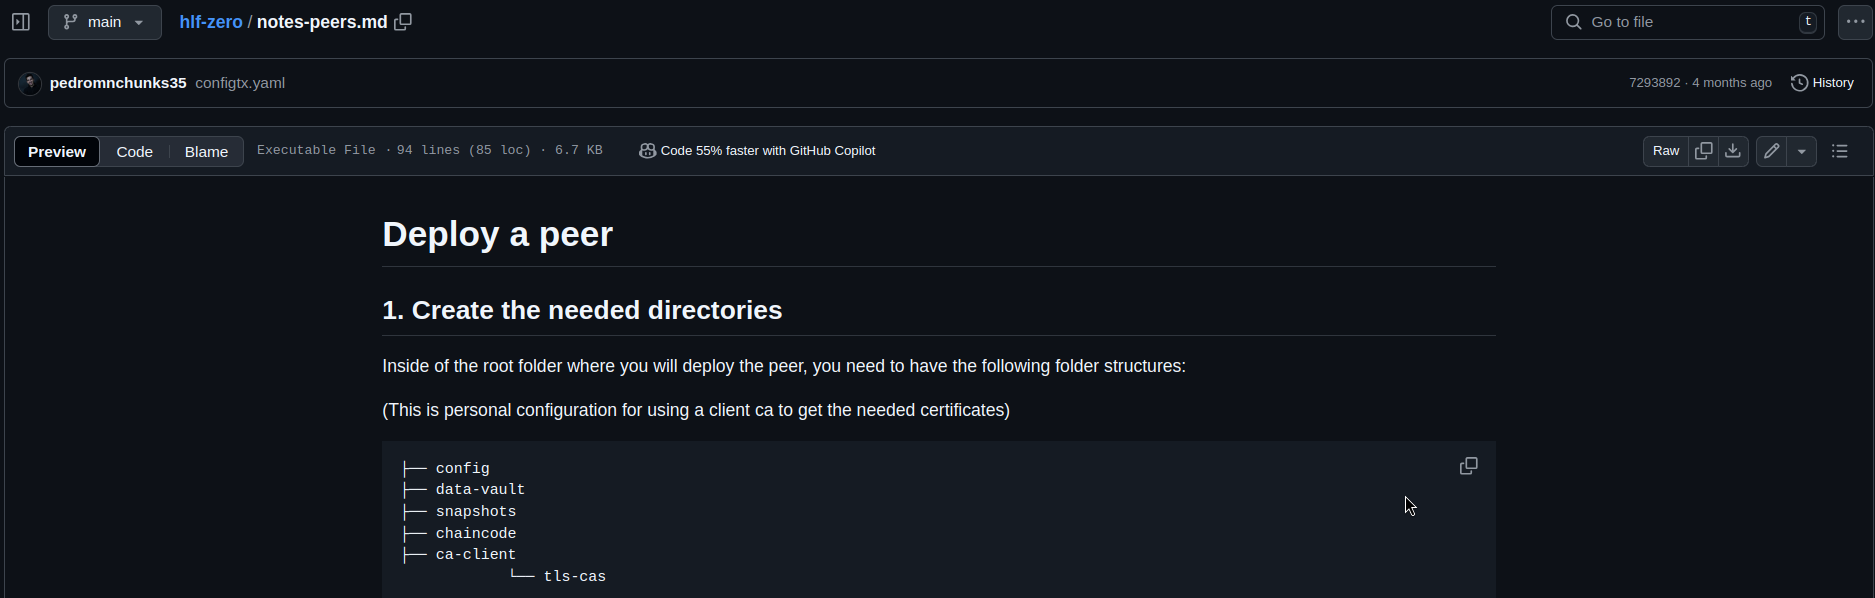
\includegraphics[width=0.5\textwidth]{assets/use-case-2/notes-peers.png} % Change this to your image file
    \caption{Second use case: peer operational guide}
    \label{fig:sample-image} 
\end{figure}

In the fifth, the focus was more into creating a configuration file for the creation of a channel. This was important for actually create means for orderers and peers know how they should communicate with each other. In the operational guide, the focus was into reviewing policies and understand how to actually setup a configuration file which is something complex that requires lots of planning. This step took a while since mistakes in the previous settled cryptographic identities could lead to errors. 

\begin{figure}[H]
    \centering
    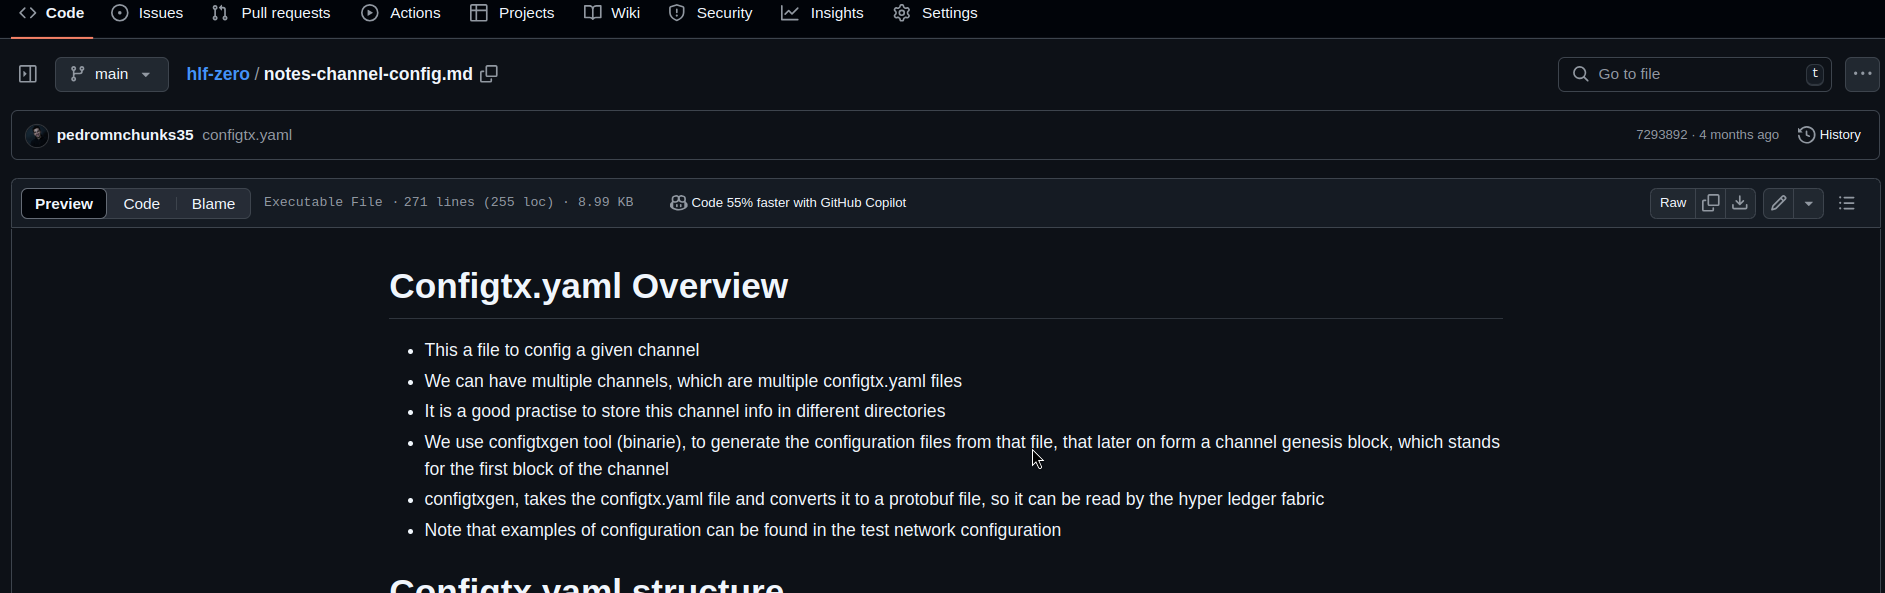
\includegraphics[width=0.5\textwidth]{assets/use-case-2/notes-channel.png} % Change this to your image file
    \caption{Second use case: channel operational guide}
    \label{fig:sample-image} 
\end{figure}

In the final operational guide, the \textbf{chaincode} was the most targeted matter.  It explains how to create a channel and how to deploy the chaincode in it, showing various phases of the chaincode life-cycle.

\begin{figure}[H]
    \centering
    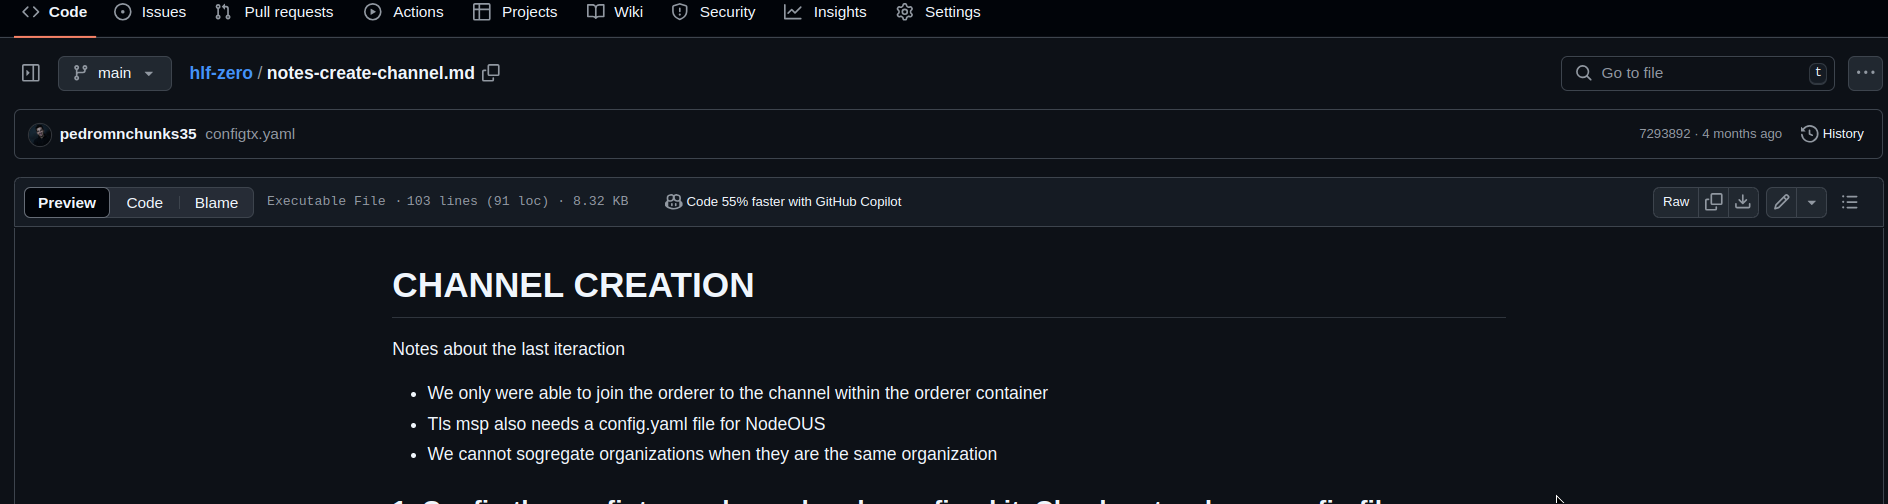
\includegraphics[width=0.5\textwidth]{assets/use-case-2/notes-channel-and-chaincode.png} % Change this to your image file
    \caption{Second use case: chaincode operational guide}
    \label{fig:sample-image} 
\end{figure}

Leveraging all of this, knowledge for the creation of a prototype network was gathered, serving as the most important base for constructing everything that would be concluded during this project.

\paragraph{5º Phase: Creating the first network}\mbox{}\\

In the phase 5, the knowledge that came from the previous phase came handy, enabling the creation of the first network prototype. Additionally, all of this was created within a personal machine by leveraging both the machine and 2 virtual machines which formed together the standardized network composed of 3 peers,1 orderer,1 CA,1 tls CA and 1 intermedium CA in the first machine, 1 orderer and 2 peers in the second machine and 1 orderer in the third machine. To simplify everything each machine was a different organization.

\begin{figure}[H]
    \centering
    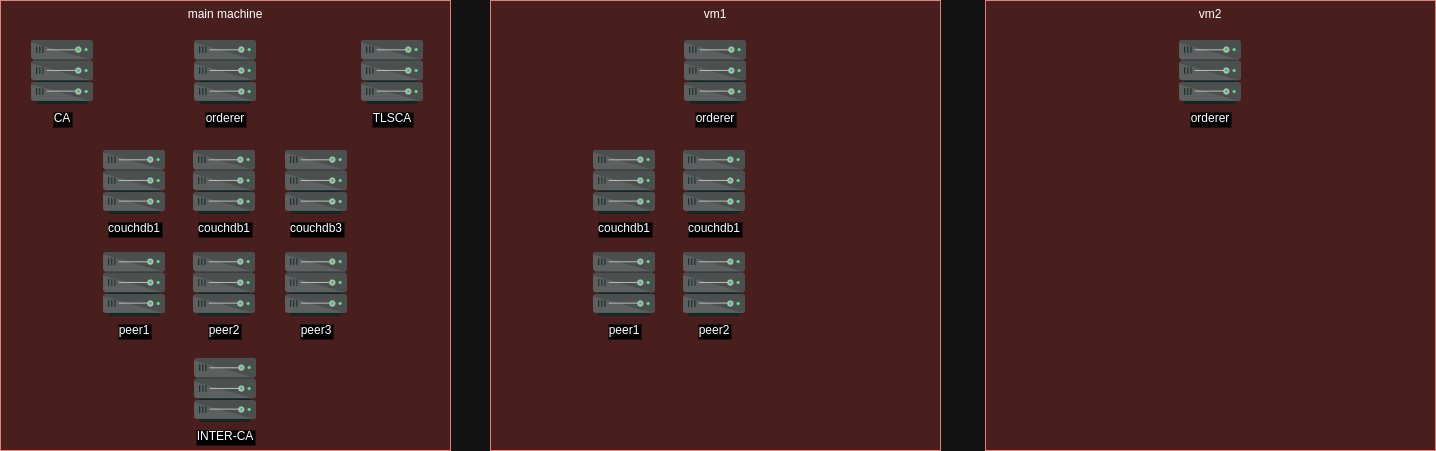
\includegraphics[width=0.5\textwidth]{assets/use-case-2/default-first-netwrk.drawio.png} % Change this to your image file
    \caption{Second use case: first network}
    \label{fig:sample-image} 
\end{figure}

Additionally, it is important to mention that a very basic chaincode was created at this stage that served for later instances of our project, where benchmarking was necessary.

\paragraph{6º Phase: First installation in a hospital}\mbox{}\\

After the first creation of a network, there was the intention to try to deploy a network in the hospital machines that were assigned to this project. Unfortunelly at the beginning there were only 2 machines available, which caused a modification of the previous network, giving origin to a default first network where the same number of components were spread in 2 machines, machine69 and machine70. The machine69 had 1 orderer,2 peers,1 CA, 1 CA for tls and 1 intermedium CA and the machine70 had 2 orderers and 2 peers. Aditionally, it should be known that all components from machine69 were cryptographically from a organization and in the machine70 cryptographically 1 orderer and 2 peers were from a second organization,while having 1 orderer from a third organization, much like the first network but without having a third machine.
\begin{figure}[H]
    \centering
    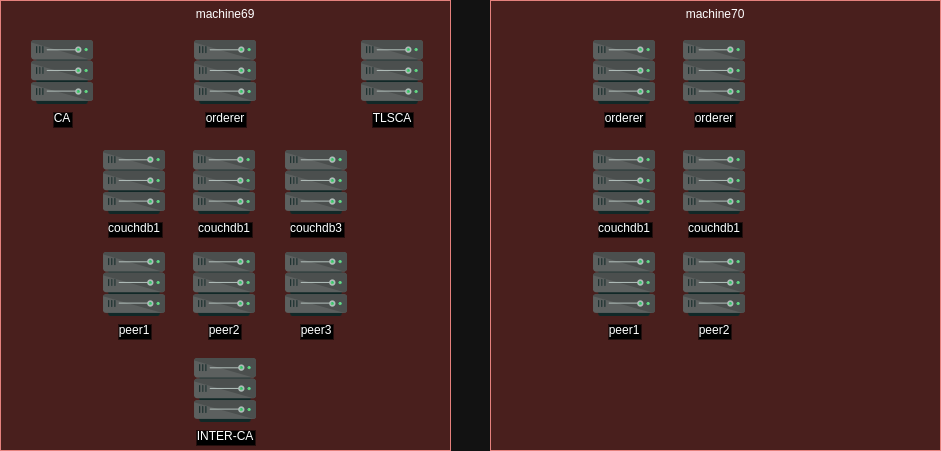
\includegraphics[width=0.5\textwidth]{assets/use-case-2/default-first-hospital.drawio.png} % Change this to your image file
    \caption{Second use case: first hospital network}
    \label{fig:sample-image} 
\end{figure}

\paragraph{7º Phase: Creating a more robust network}\mbox{}\\
Thinking in the next iteration, here there was an adaptation of an existing blockexplorer from Hyperledger fabric for the prototype demonstration. Also, there was a refinement of the previous structure of the configuration files from the guidelines, resulting in a template. This template was done according to a set of scripts that were developed. One script was to generate all of the configurations for a given component according to its type (ledger, peer, and orderer), enabling deterministic creation of new components if needed; another script was in charge of putting these configurations in the desired machine; and the third script was to deploy the desired components while still maintaining previous configurations of components in the machine, enabling to reset the network to any structure of network that was specified in a file with a specific syntax, which was a must for further usage in benchmarking, where different networks were tested, always created from scratch.
\begin{figure}[H]
    \centering
    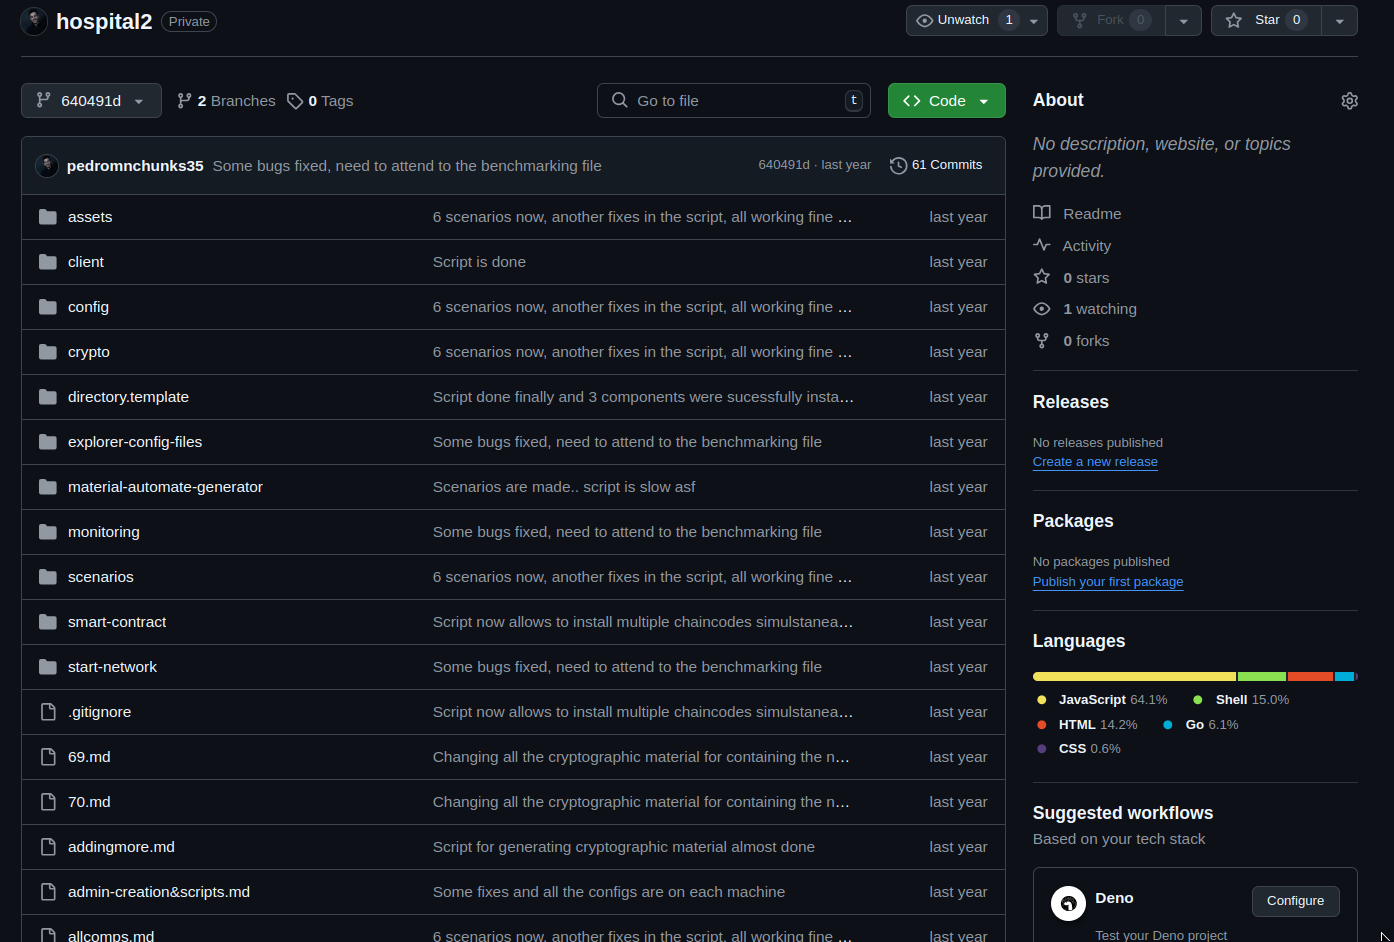
\includegraphics[width=0.5\textwidth]{assets/use-case-2/robust-network-creation.png} % Change this to your image file
    \caption{Second use case: hospital v2 repository}
    \label{fig:sample-image} 
\end{figure}
In the given picture, it can be spotted that there is a directory for templates (directory.template), a directory for scripts that generate new configurations  and transfers them to a desired machine (material-automate-generator) and there is a directory for resetting a network making different networks out of the box (start-network).

\paragraph{8º Phase: Prototype demonstration}\mbox{}\\
At this stage, there was the need to present a prototype of the network. Since the spectators were not technical, recursion to a block explorer was necessary, such that until an own implementation surged, a legacy version was used and the presentation went smoothly.

\paragraph{9º Phase: Interim report delivery} \mbox{}\\
During this phase the report that started before was delivered, such that some fixes were needed before being actually accepted by the responsibles.

\paragraph{10º Phase: Dissertation development}\mbox{}\\
Within the 10th phase realm, the dissertation started to exist and got incremented in terms of content as the time was progressing, making sure that the schedules were being fulfilled and the project was running accordingly to the expectations.

\paragraph{11º Phase: Studying Benchmarking}\mbox{}\\
This was the phase where \textbf{caliper},\textbf{cadvisor},\textbf{prometheus} and \textbf{grafana} were under inspection. \textbf{Cadvisor} was used to expose time series data relative to performance metrics of the machine, \textbf{caliper} is the actual benchmark performer, \textbf{prometheus} is where the data from cadvisor will be gathered to be used in \textbf{grafana} which creates a visualization.

\paragraph{12º Phase: Making a benchmark locally}\mbox{}\\
In this phase,a whole dashboard for visualizing and extracting data was created with grafana and a benchmarking was done in a local network. This local network was the one that was created in the first instance and this benchmark was only to make sure that everything was working as expected.  

\begin{figure}[H]
    \centering
    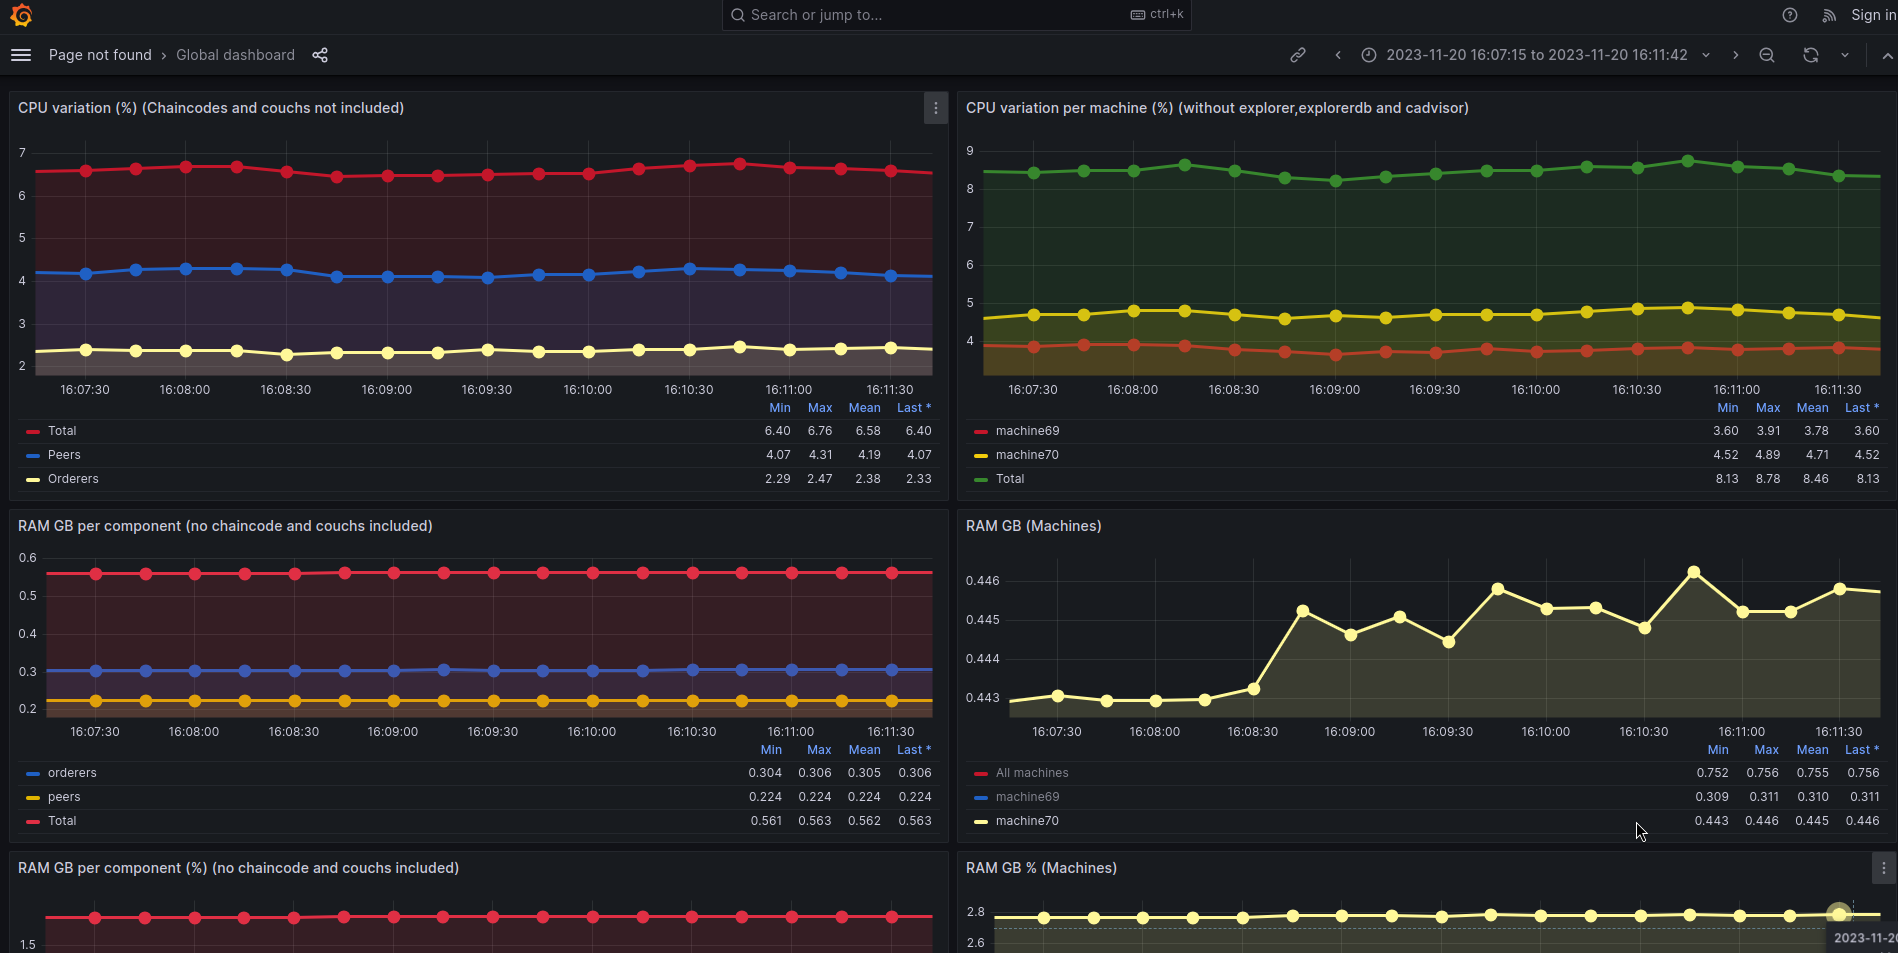
\includegraphics[width=0.5\textwidth]{assets/use-case-2/first-benchmarking.png} % Change this to your image file
    \caption{Second use case: first benchmark}
    \label{fig:sample-image} 
\end{figure}

\begin{figure}[H]
    \centering
    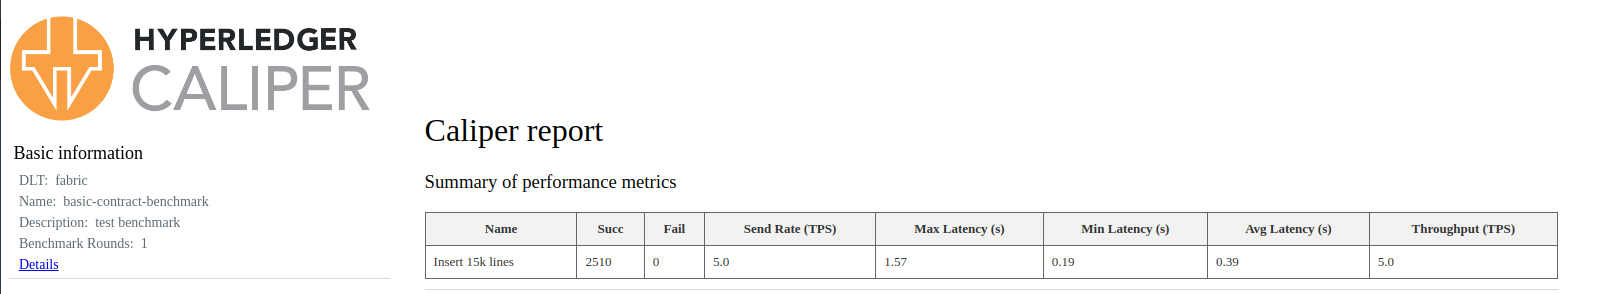
\includegraphics[width=0.5\textwidth]{assets/use-case-2/first-benchmarking2.png} % Change this to your image file
    \caption{Second use case: first benchmark (part 2)}
    \label{fig:sample-image} 
\end{figure}

\paragraph{13º Phase: Benchmarking the first network}\mbox{}\\
After having everything tested in a local environment, a real benchmark over the first hospital network was conducted. This time, the data was actually extracted as CSV. This is because it becomes easier to create graphics that are more eager to be interpreted by paper, while the one's created are better for dynamic analysis which is fine but not for scientific work. The benchmarks were yield 10 times to make sure that it was not a one time occasion.
\begin{figure}[H]
    \centering
    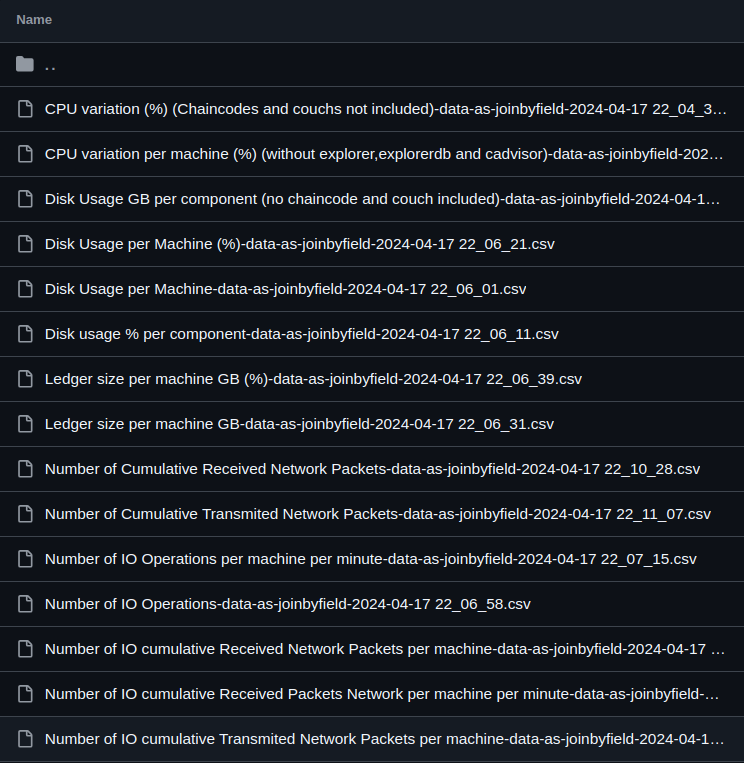
\includegraphics[width=0.5\textwidth]{assets/use-case-2/first-benchmarking-hospital.png} % Change this to your image file
    \caption{Second use case: first benchmark hospital}
    \label{fig:sample-image} 
\end{figure}

\begin{figure}[H]
    \centering
    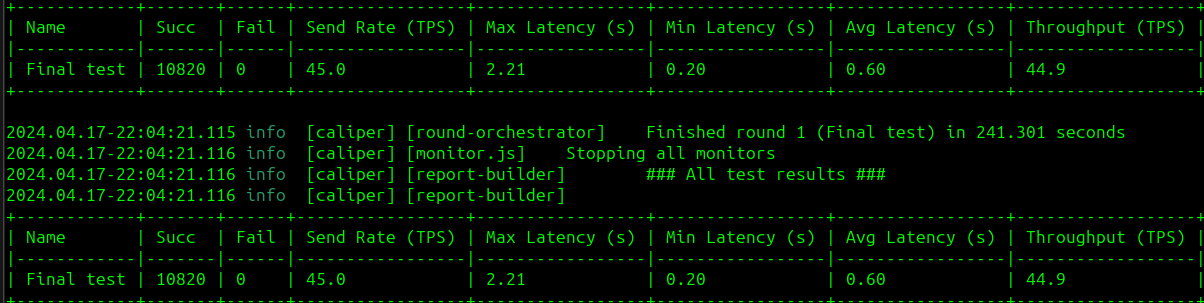
\includegraphics[width=0.5\textwidth]{assets/use-case-2/first-benchmarking-hospital2.png} % Change this to your image file
    \caption{Second use case: first benchmark hospital (part 2)}
    \label{fig:sample-image} 
\end{figure}

\begin{figure}[H]
    \centering
    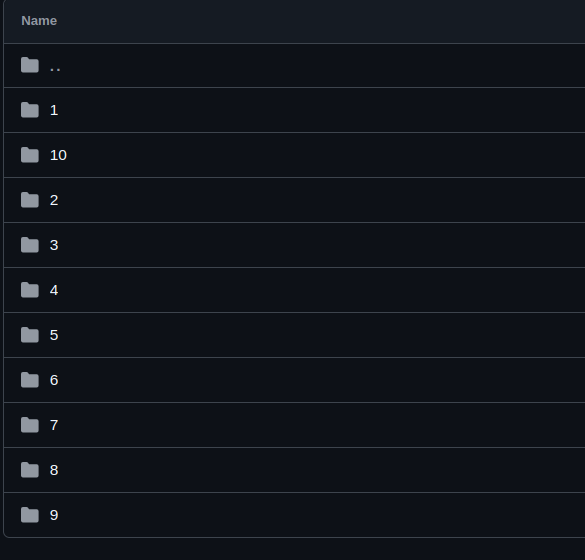
\includegraphics[width=0.5\textwidth]{assets/use-case-2/first-benchmarking-hospital3.png} % Change this to your image file
    \caption{Second use case: first benchmark hospital (part 3)}
    \label{fig:sample-image} 
\end{figure}
\paragraph{14º Phase: Studying Kubernetes}\mbox{}\\
After benchmarking a normal bare metal network, there was a deep reflection about the ease to use such infrastructure. Between configuring everything and putting everything in every single machine and managing every single instance within a healthcare organization, it became obvious that it would create burden for a administrator that wanted to spoil it's machines with multiple components. 

With this in mind, within this phase there was a deep dive into kubernetes. Very powerful as it is, it imposed a very huge challenge in terms of knowledge as the \textbf{hyperledger fabric}, where the documentation was very complete and extensive, not speaking about the tutorials that were done in order to understand the basis of such tool. In addition, this became even more clear with the fact that the infrastructure had the need to be implemented on premise, where everything must be installed from scratch, different from the cloud where everything is already installed and ready to use.

Besides \textbf{kubernetes}, other technologies were observed for the on-premise imposition. This technologies were \textbf{metallb},\textbf{calico} and \textbf{kubeadm}. \textbf{Metallb} was required to offer load balancing capabilities, \textbf{calico} was a network plugin for pods to communicate with each other and \textbf{kubeadm} was to deploy and join nodes to a cluster.

Relatively to operational guides and abstracts of what was covered during this interval, they were placed in github repositories where information was both by photo and markdown files making this information accessible whenever needed.

\begin{figure}[H]
    \centering
    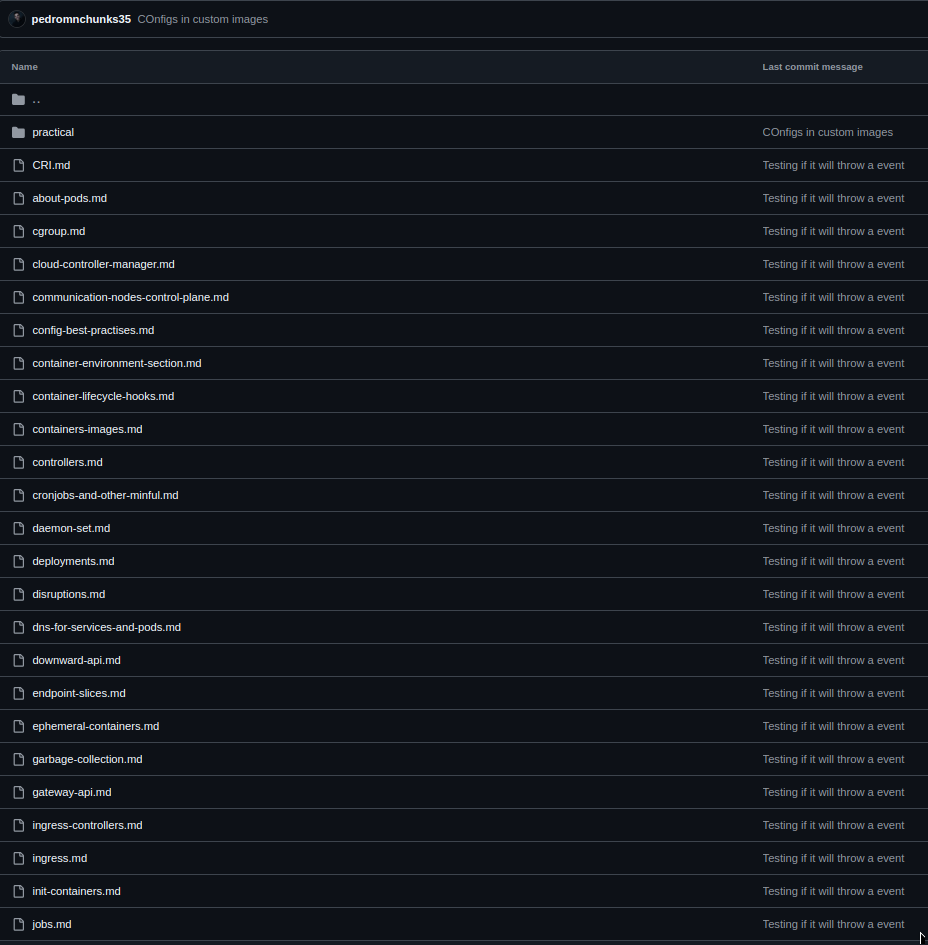
\includegraphics[width=0.5\textwidth]{assets/use-case-2/kubernetes-study.png} % Change this to your image file
    \caption{Second use case: kubernetes study}
    \label{fig:sample-image} 
\end{figure}

\begin{figure}[H]
    \centering
    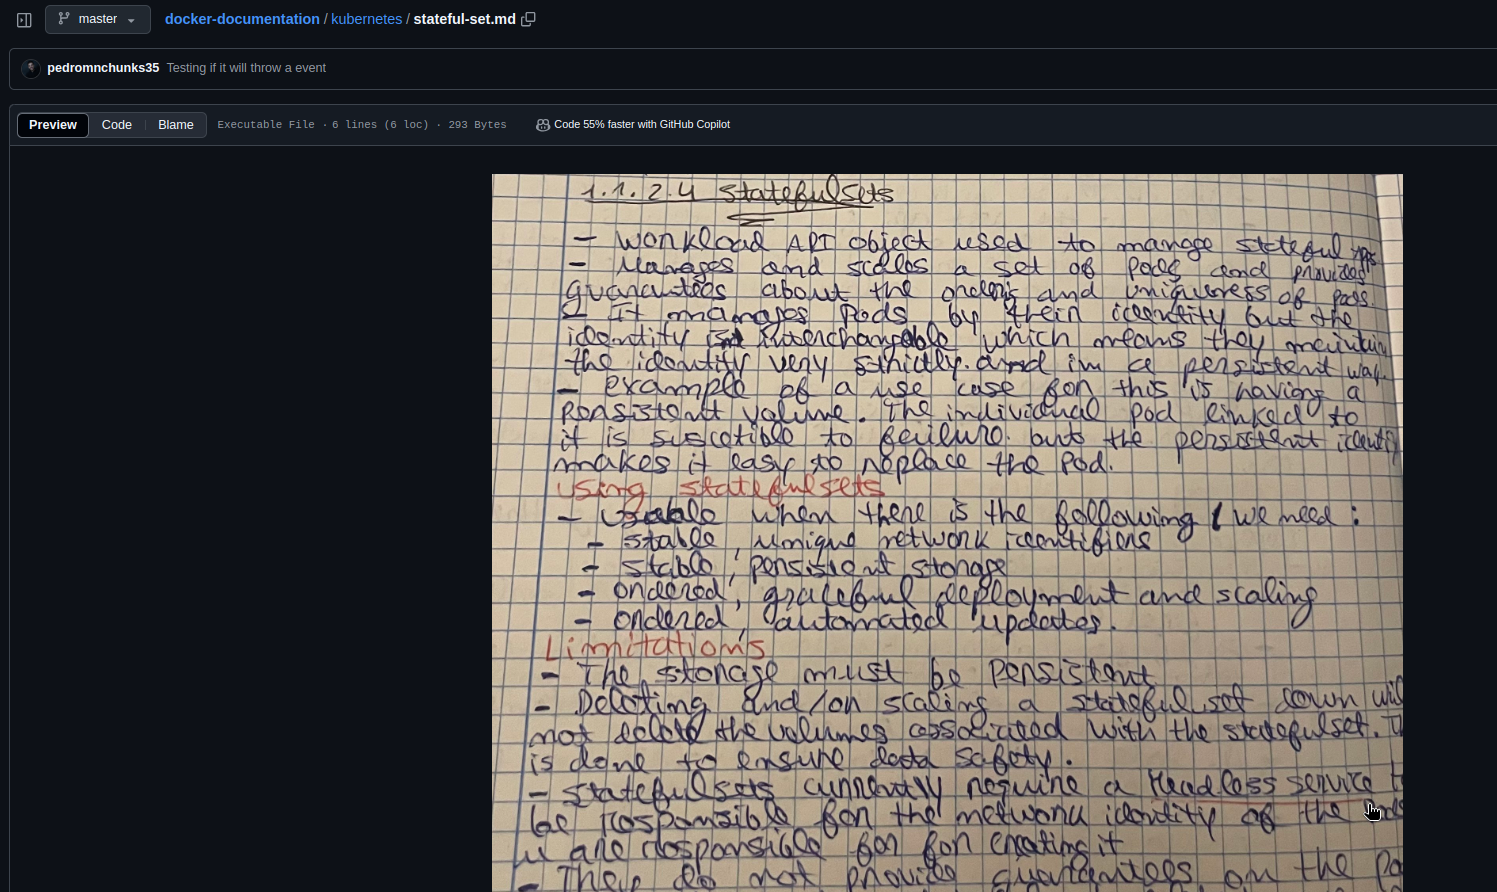
\includegraphics[width=0.5\textwidth]{assets/use-case-2/kubernetes-study2.png} % Change this to your image file
    \caption{Second use case: kubernetes study (handwriten)}
    \label{fig:sample-image} 
\end{figure}

\paragraph{15º Phase: Implementing a blockchain network with kubernetes}\mbox{}\\
In this phase, a \textbf{hyperledger fabric} network was built under \textbf{kubernetes}. To achieve this, this network was deployed firstly locally with the main machine as the master node and 1 VM as it's slave node. The network that was deployed there was relatively small compared to the first that was deployed in the local environment and no load balancer was implemented in this inception because the objective was to simply put a network in such environment. Additionally, it should be known that in \textbf{hyperledger fabric}, deploying a chaincode in bare metal is completely different from implementing it in a \textbf{kubernetes} environment: In a bare metal environment the installation of the peer can be done directly in the peer, while in the case of kubernetes chaincode must be installed as a service that can be shared by multiple peers. The reason for this has to do with the control over the container runtime. There are operational guidelines regarding this first implementation.

\begin{figure}[H]
    \centering
    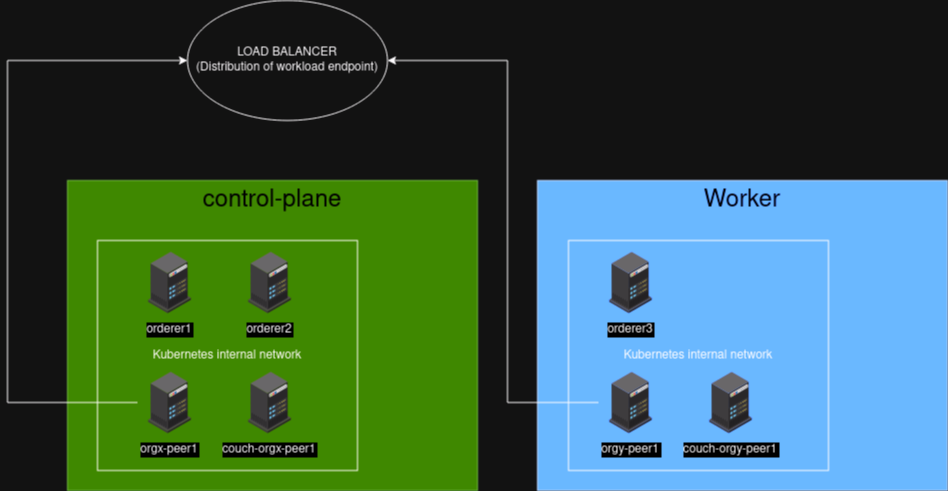
\includegraphics[width=0.5\textwidth]{assets/use-case-2/hlf-kuber-premise-network.png} % Change this to your image file
    \caption{Second use case: local kubernetes hlf network}
    \label{fig:sample-image} 
\end{figure}

\begin{figure}[H]
    \centering
    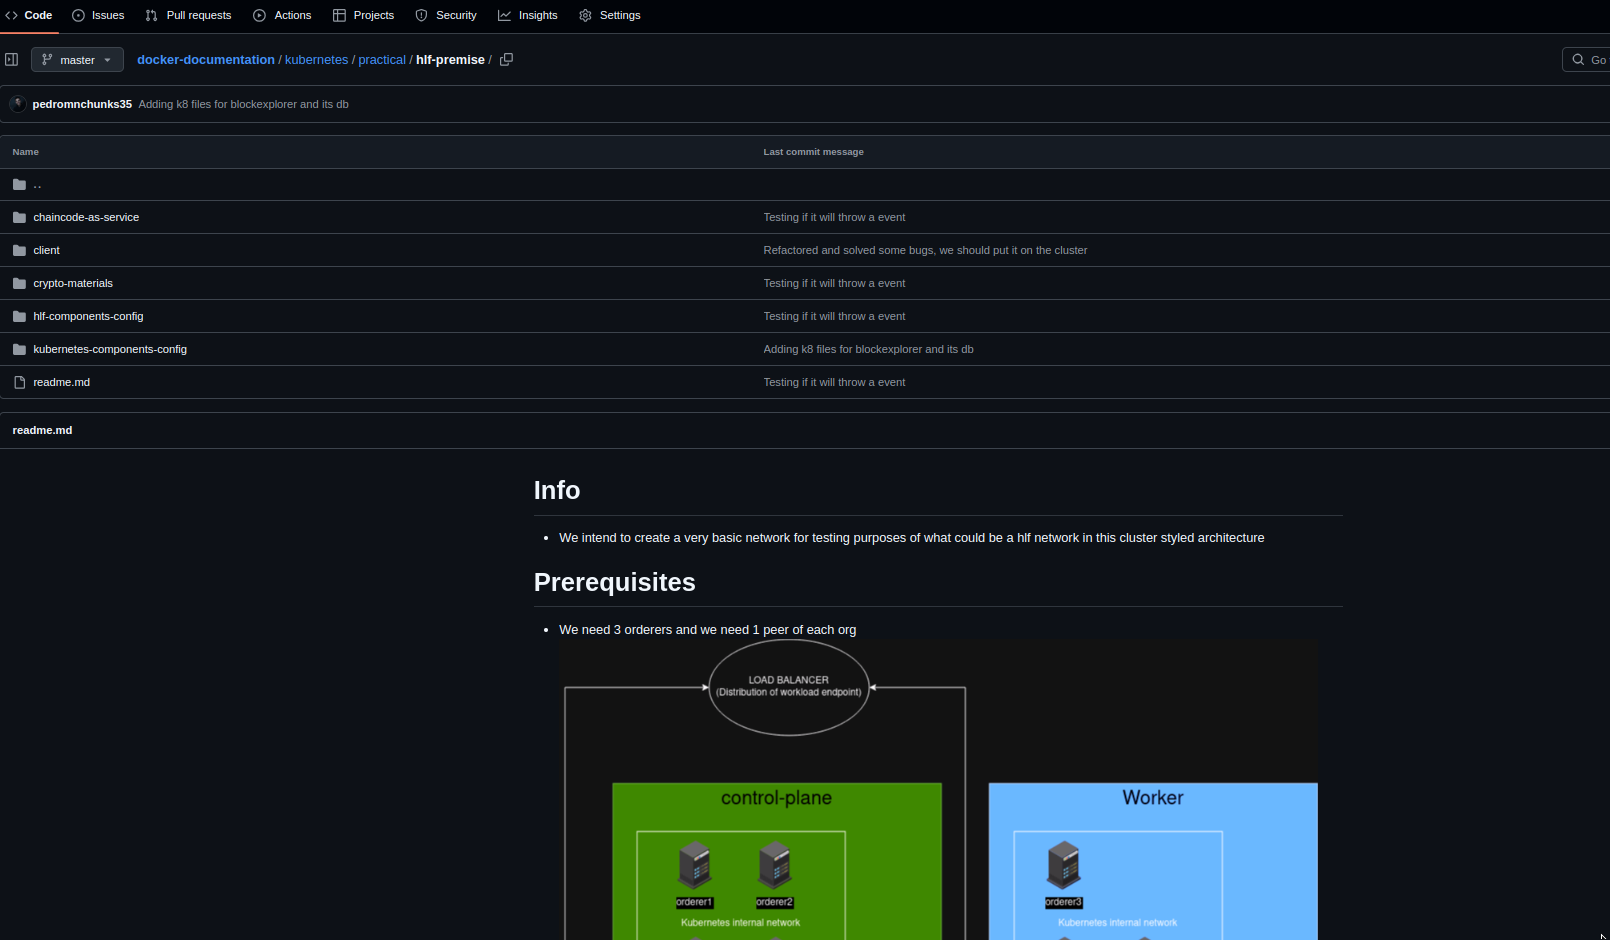
\includegraphics[width=0.5\textwidth]{assets/use-case-2/hlf-kuber-premise-network2.png} % Change this to your image file
    \caption{Second use case: local kubernetes hlf network (part 2)}
    \label{fig:sample-image} 
\end{figure}

It should be noted that despite a reference to a load balancer in the network structure image, there is no real load balancer but rather a nodePort which also does load balancing but in a limited way since that is not it's main purpose.

\paragraph{16º Phase: Creating a more robust network for a kubernetes environment}\mbox{}\\
After accomplishing a working \textbf{kubernetes} network, 2 things were added to provide more support to the network and a third thing was added just for testing. Firstly, a real load balancer that supports on-bare metal kubernetes was deployed which was the previous mentioned \textbf{metallb}. In second, Automation mechanisms were also added to contribute to reseting and managing the network more effectively but with it's aim in adding in the future a UI that could give an administrator the power to manage it's infrastructure. Lastly, a service mesh was implemented for testing purposes for knowing how could such practise give more grained control over the network by controlling in which cases traffic is allowed, while providing monitoring features that are very useful for an admin.

Focusing more in the second point, this was a innovative idea that came from a \textbf{Sidecar} container Architectural pattern. This was the case, since every component of the network has a side-container to extend it's communication features, enabling to upload files and also to run commands destined to the binaries exactly like the admin would be inside of the container. During this phase, a web UI prototype was also used to test this features and this way of communicating with every service was also widely used to automate network booting alongside with scripts which would also automate multiple network schemes to the network, just like it was done in the on bare-metal approach but in a even more easier to use methodology, since with this there is the opportunity to use a general purpose programming language such as golang or javascript. 

During this conception, another structure of network was implemented, presenting 3 machines instead of only 2, where there was a control plane with a single point of failure graphql service and 1 peer with a side container and a orderer with a side container in each machine forming all together a cluster locally where an administrator could run commands easily.

\begin{figure}[H]
    \centering
    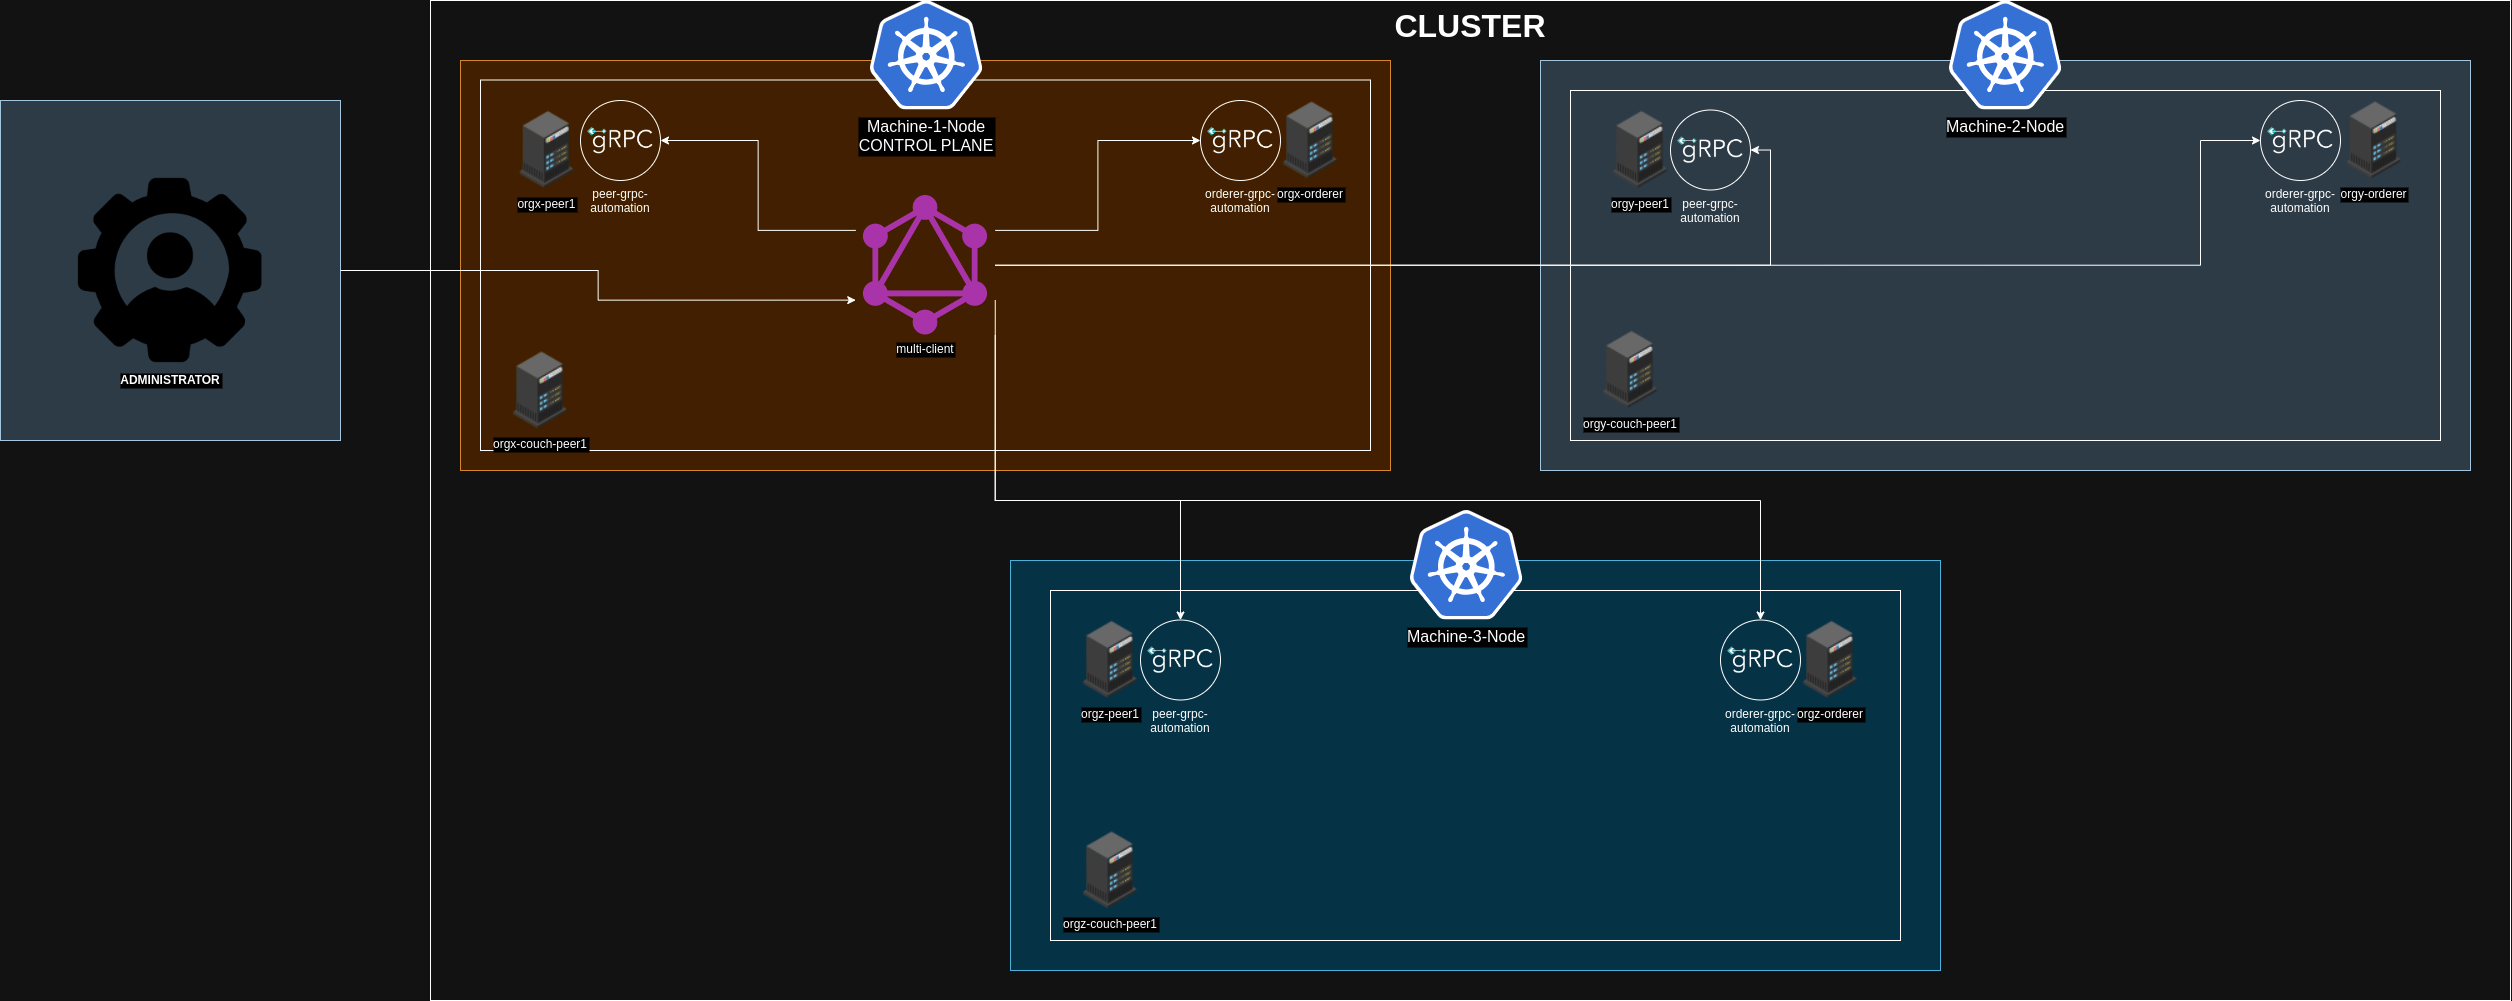
\includegraphics[width=0.5\textwidth]{assets/use-case-2/automation-diagram.drawio.png} % Change this to your image file
    \caption{Second use case: kubernetes automation creation}
    \label{fig:sample-image} 
\end{figure}

\begin{figure}[H]
    \centering
    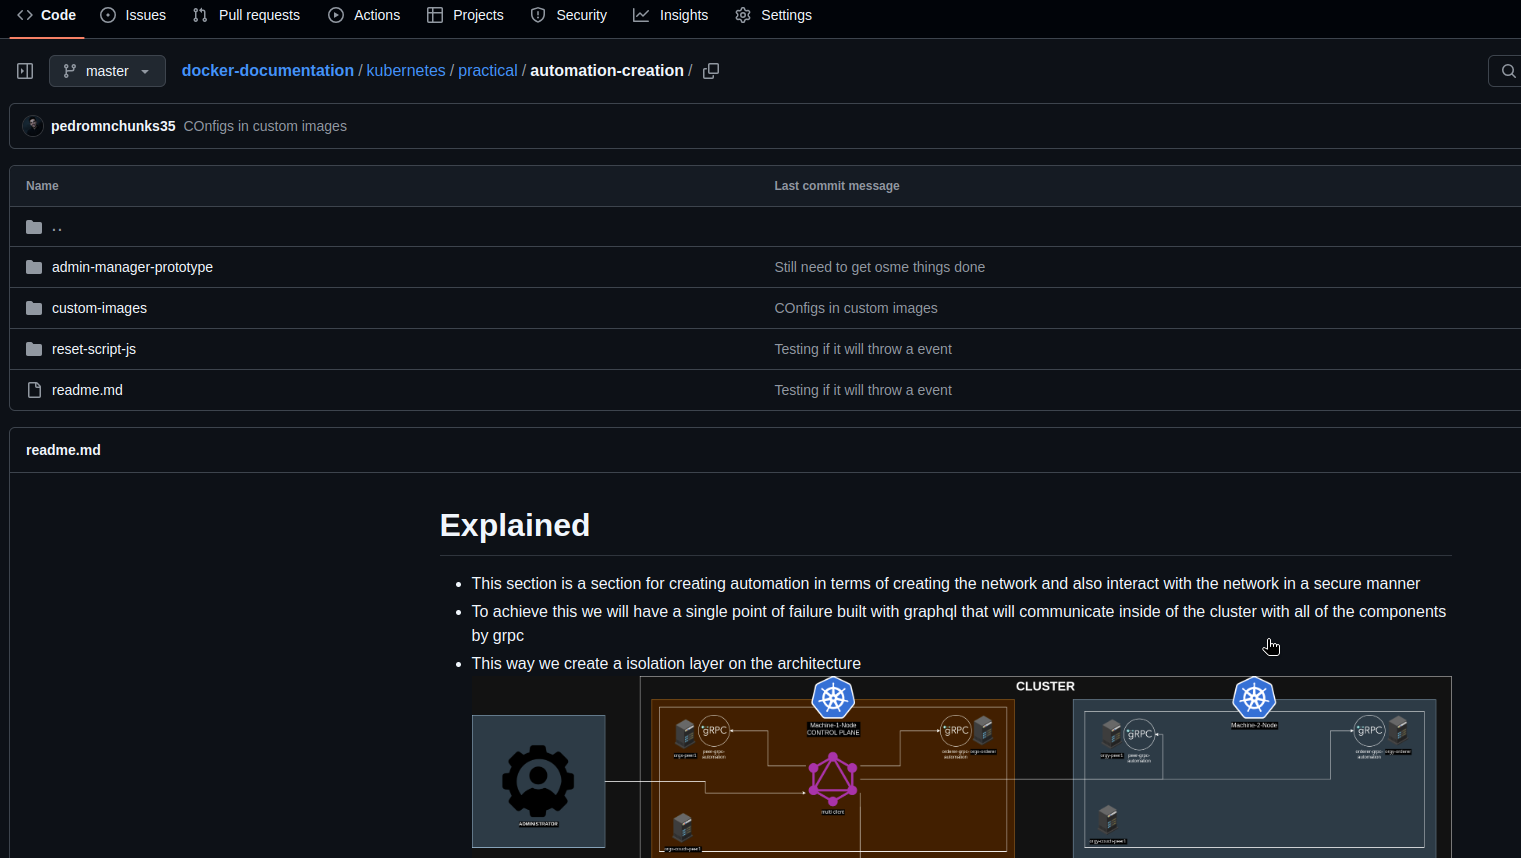
\includegraphics[width=0.5\textwidth]{assets/use-case-2/automation-creation.png} % Change this to your image file
    \caption{Second use case: kubernetes automation creation repository}
    \label{fig:sample-image} 
\end{figure}

\begin{figure}[H]
    \centering
    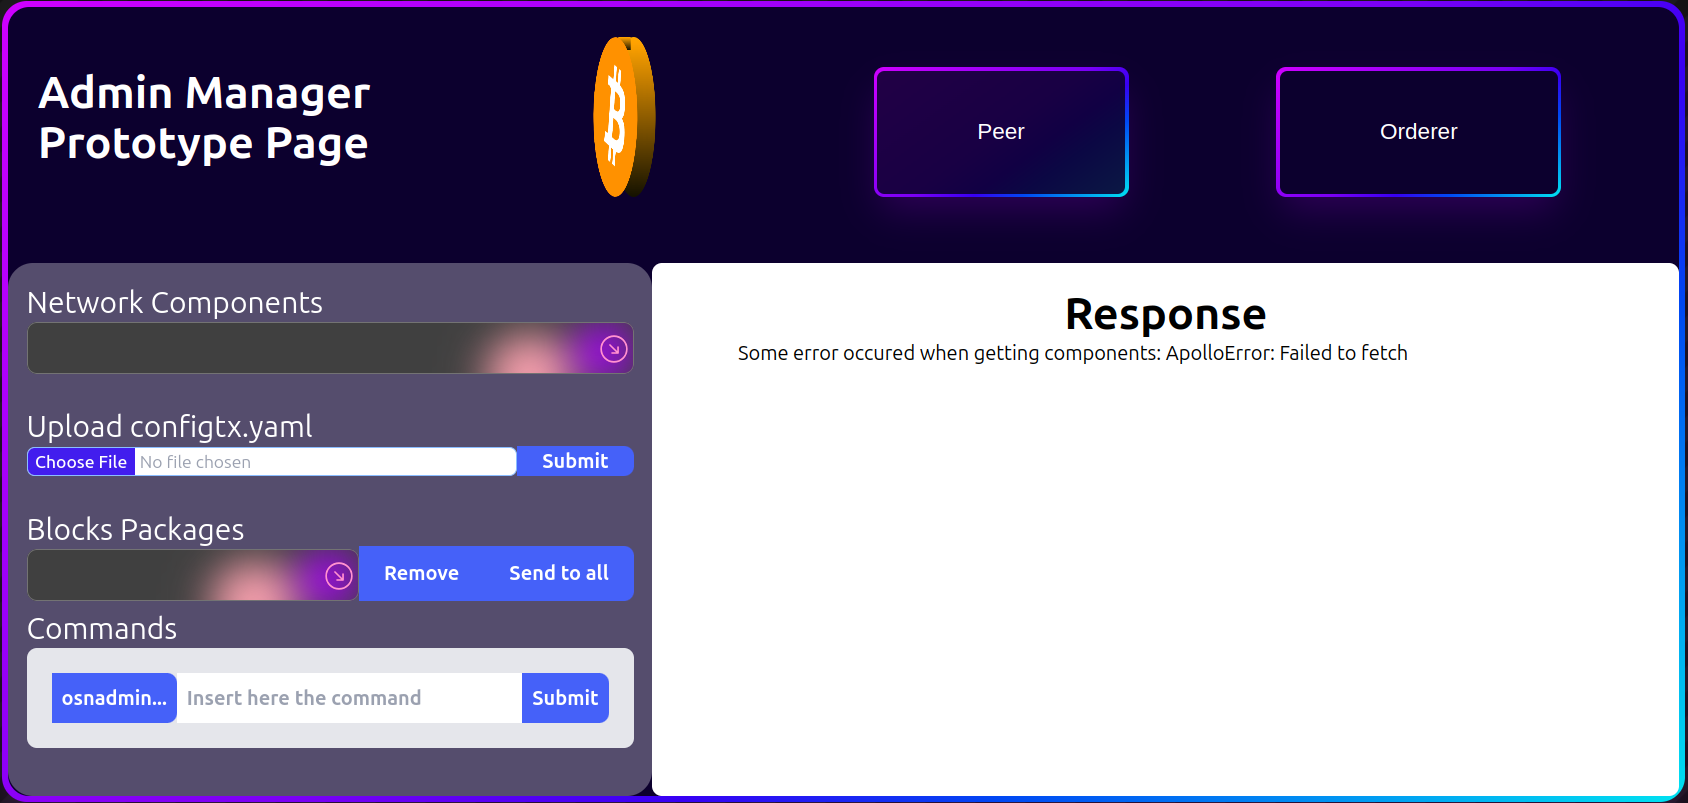
\includegraphics[width=0.5\textwidth]{assets/use-case-2/orderer-admin-manager.png} % Change this to your image file
    \caption{Second use case: kubernetes automation creation orderer prototype}
    \label{fig:sample-image} 
\end{figure}

\begin{figure}[H]
    \centering
    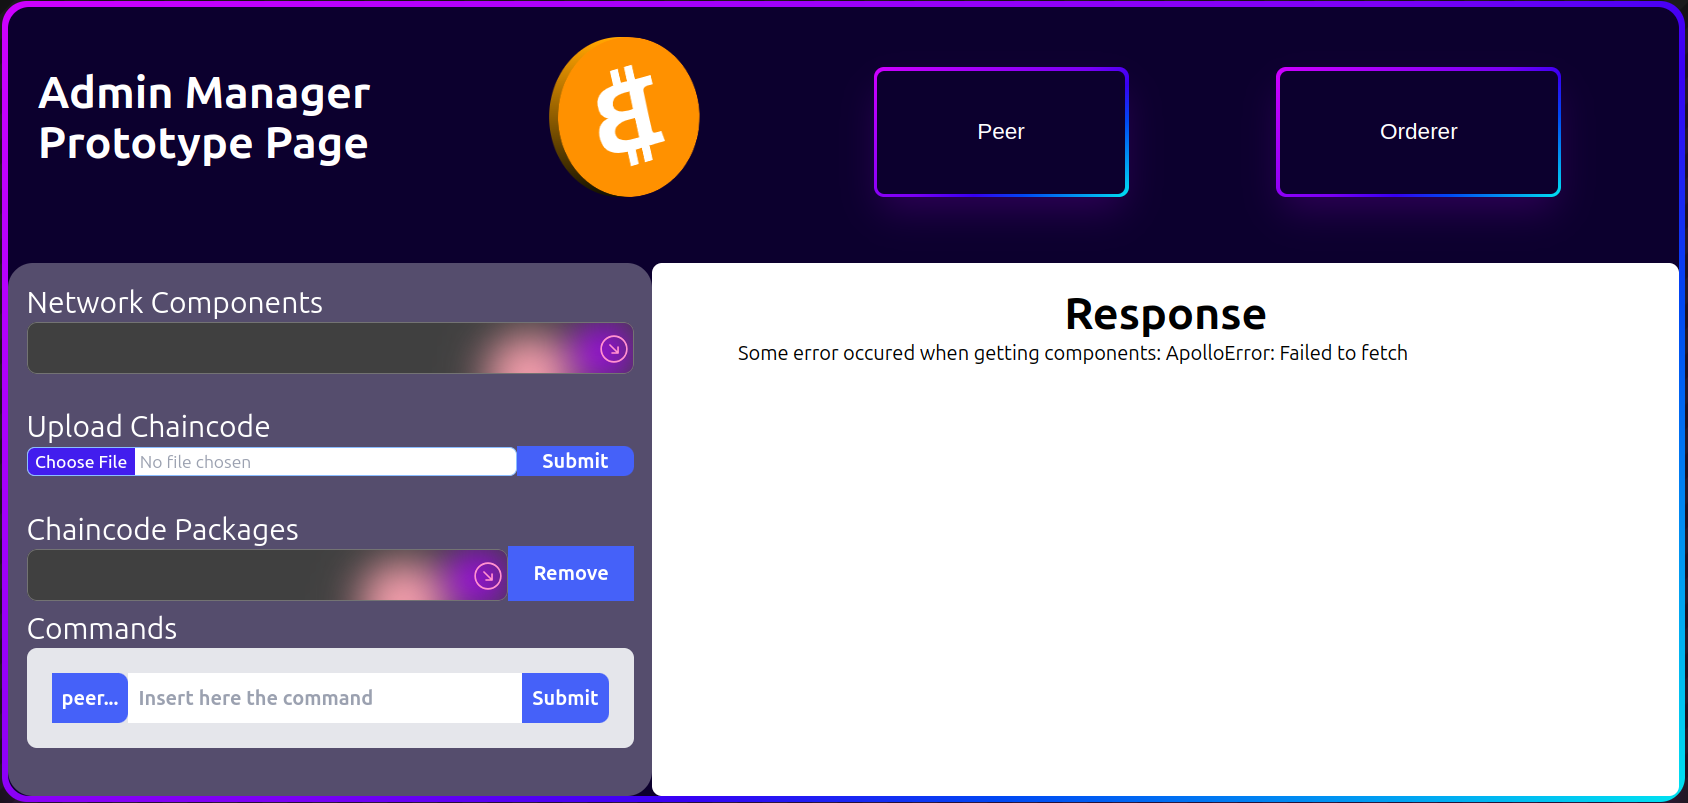
\includegraphics[width=0.5\textwidth]{assets/use-case-2/peer-manager-prototype-page.png} % Change this to your image file
    \caption{Second use case: kubernetes automation creation peer prototype}
    \label{fig:sample-image} 
\end{figure}

\paragraph{17º Phase: Second installation in a hospital}\mbox{}\\
In this phase, fortunately there was a release of an extra machine for this work which was very pertinent for what was about to come and it was even more suitable because the same network structure was already implemented in the local network. With this in mind, the same network with the same sidecar container and metallb functionalities was implemented successfully in the hospital environment, while effectively handle the segregation with \textbf{non-kubernetes} implementation by deploy a chaincode-as-service instance.
\begin{figure}[H]
    \centering
    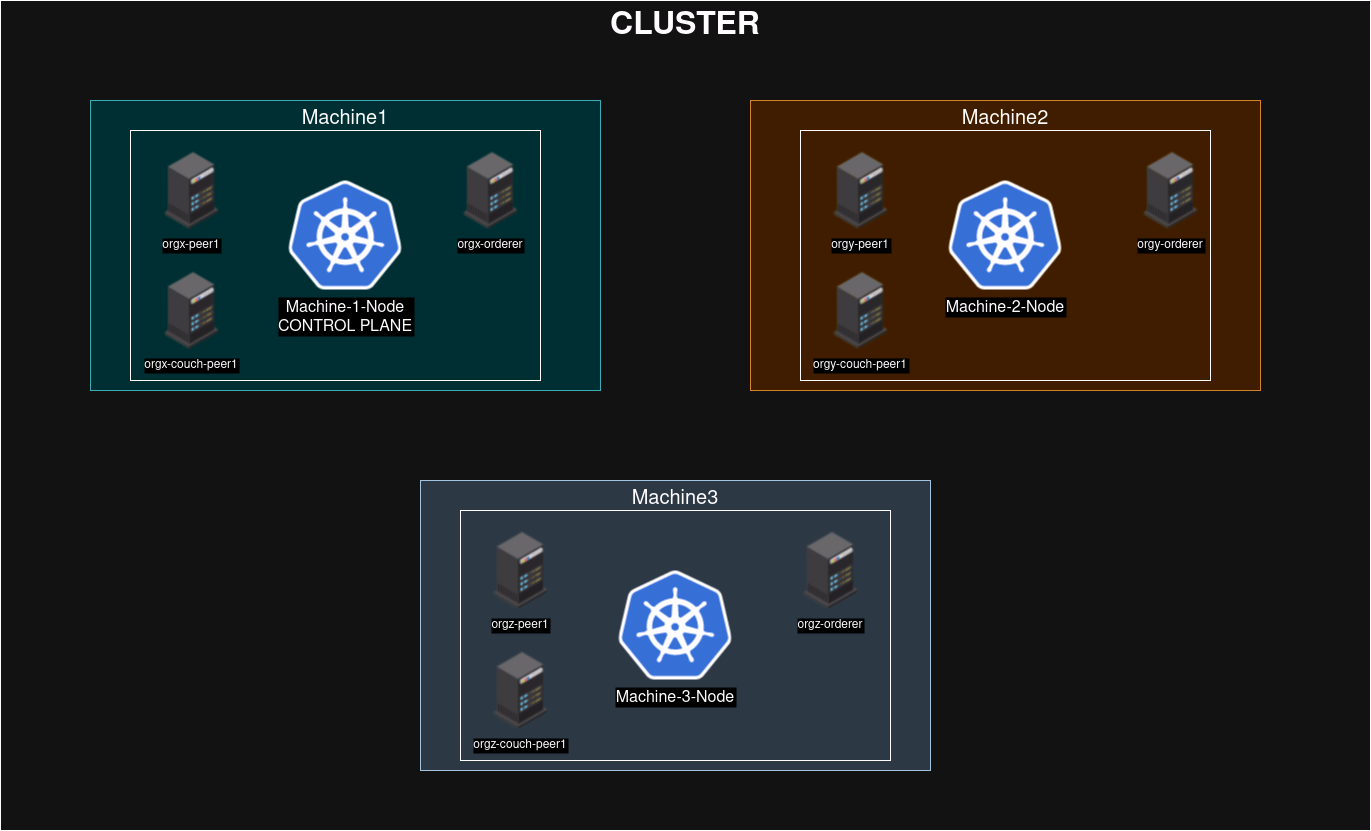
\includegraphics[width=0.5\textwidth]{assets/use-case-2/kubernetes-network.drawio.png} % Change this to your image file
    \caption{Second use case: kubernetes first hlf hospital network}
    \label{fig:sample-image} 
\end{figure}

\paragraph{18º Phase: Creation of multiple networks}\mbox{}\\
As mentioned before, the bigger the network in terms of number of different identities, the bigger the network burden. With this in mind, within this phase knowing the limitations of the number of components that could be handled by 2 machines was putted into cause. At this time, the third machine was on maintenance, which causes to only test this overhead in 2 machines instead of 3. However, to see until each measure this could impose a threat in a small set of resources it was created 6 scenarios of networks which are the following:

The default scenario, was the first scenario that was implemented in the first hospital network when there was only 2 machines: first organization had 1 orderer and 2 peers and it was located in the first machine, the second organization had 1 orderer and 3 peers and was located in the second machine and the third organization had 1 orderer and it was located in the second machine as well.

\begin{figure}[H]
    \centering
    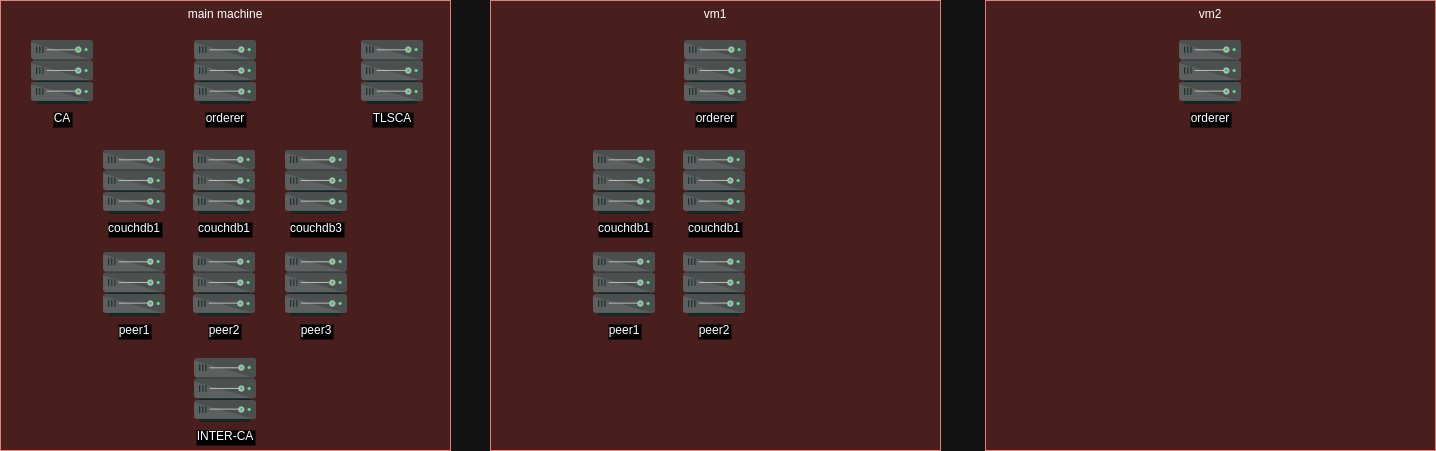
\includegraphics[width=0.5\textwidth]{assets/use-case-2/default-first-netwrk.drawio.png} % Change this to your image file
    \caption{Second use case: multiple networks default scenario}
    \label{fig:sample-image} 
\end{figure}

In the first scenario, the first machine had one organization with 1 orderer and 1 peer and the second machine had 2 organization where the first had 1 orderer and 1 peer and the second had 1 orderer.

\begin{figure}[H]
    \centering
    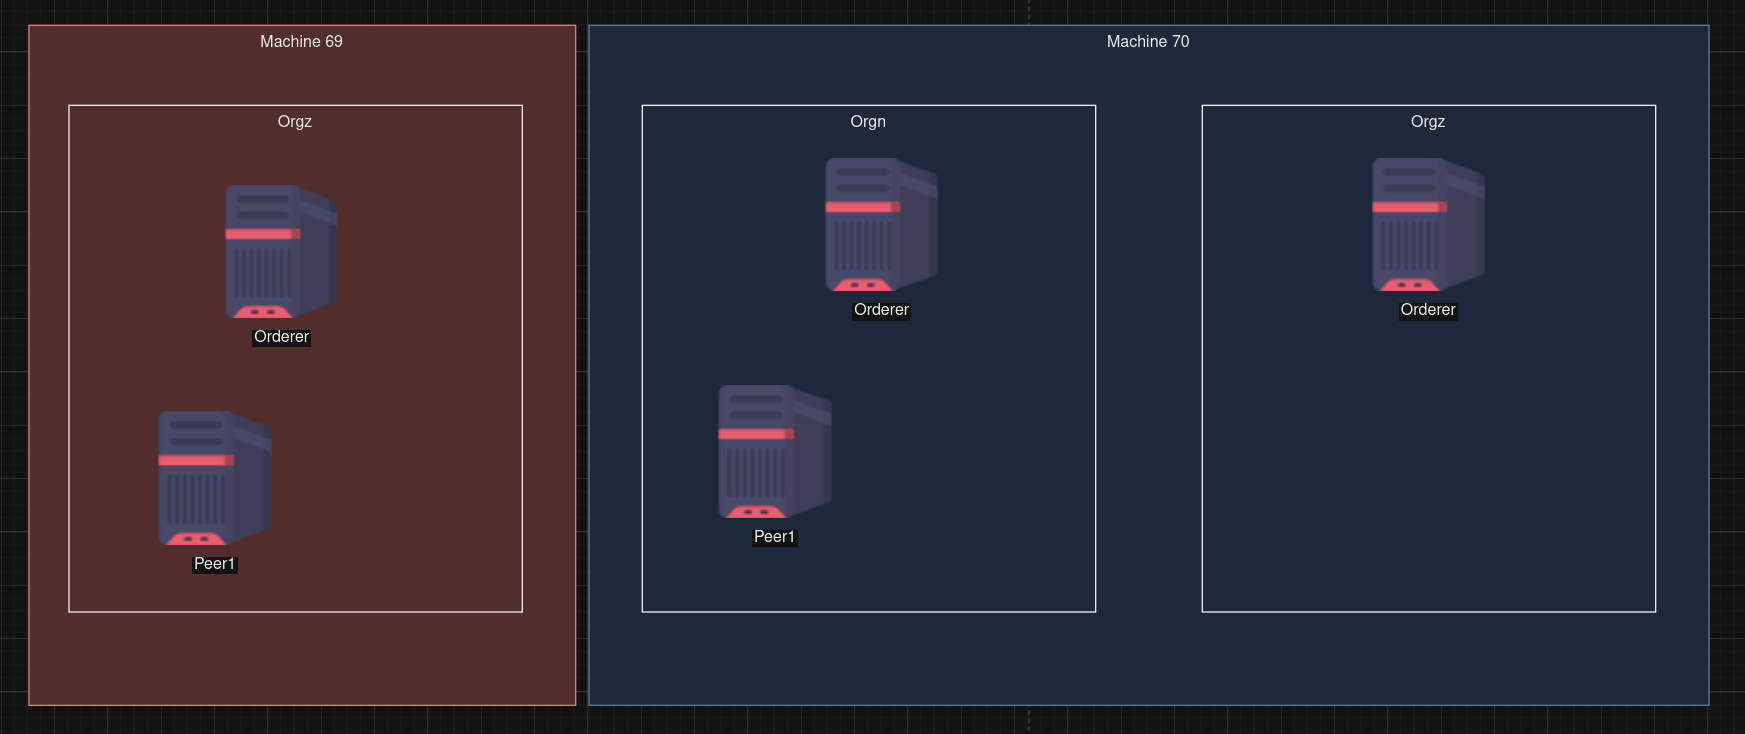
\includegraphics[width=0.5\textwidth]{assets/use-case-2/scenario1.png} % Change this to your image file
    \caption{Second use case: multiple networks scenario 1}
    \label{fig:sample-image} 
\end{figure}

Within the second scenario, in the first machine there were 3 organizations: The first one had 1 orderer, the second one had 1 orderer and the third had 1 orderer and 2 peers. Also, in the second machine there were 2 organizations: The first one had 1 orderer and 3 peers and the second one had 1 orderer.

\begin{figure}[H]
    \centering
    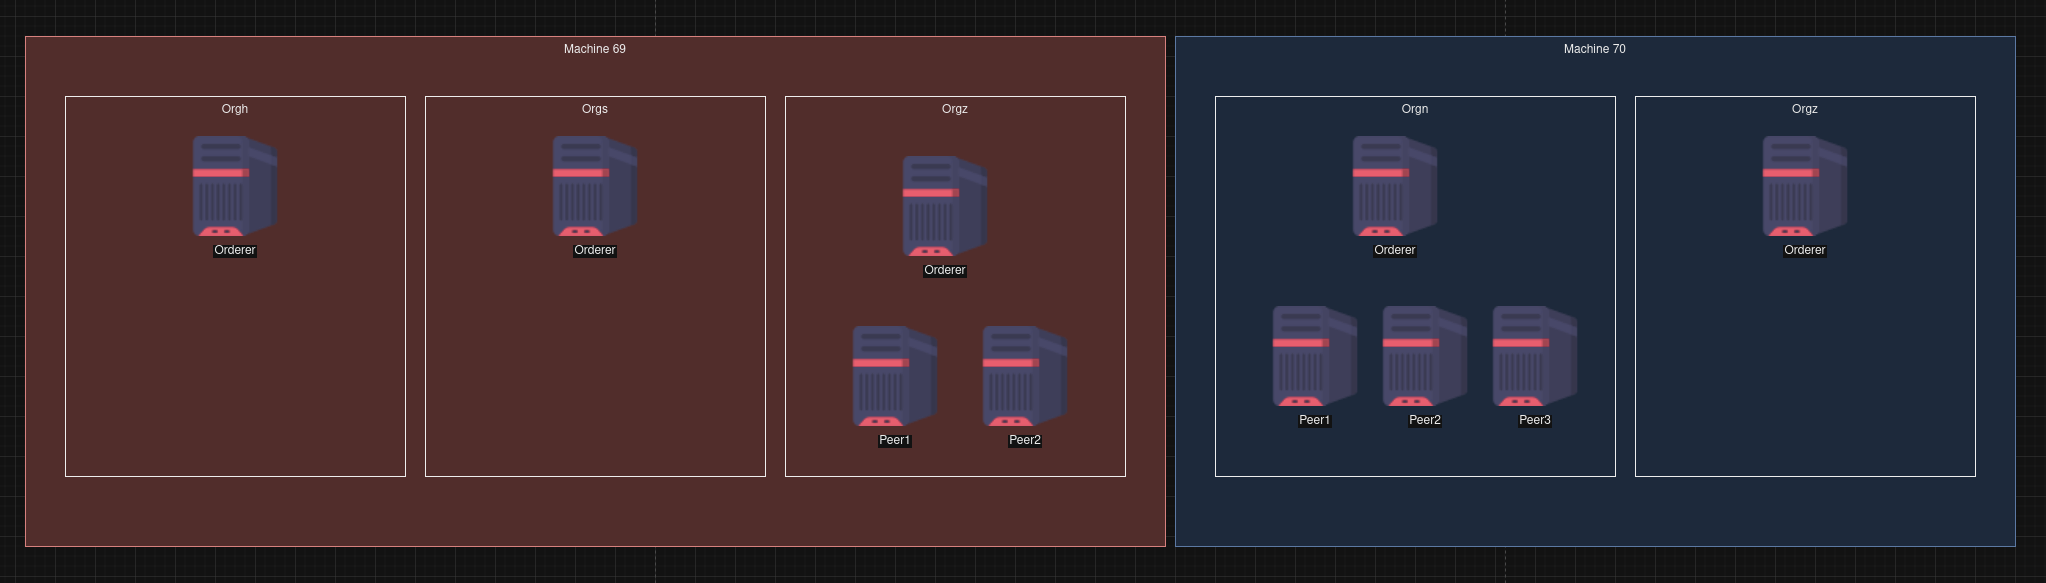
\includegraphics[width=0.5\textwidth]{assets/use-case-2/scenario2.png} % Change this to your image file
    \caption{Second use case: multiple networks scenario 2}
    \label{fig:sample-image} 
\end{figure}

In the third scenario, in the first machine there were also 3 organizations: the first had 1 orderer, the second had 1 orderer and 3 peers while the third had 1 orderer and 2 peers. In the second machine, there were 2 organizations: The first had 1 orderer and 3 peers and the second had 1 orderer and 3 peers.

\begin{figure}[H]
    \centering
    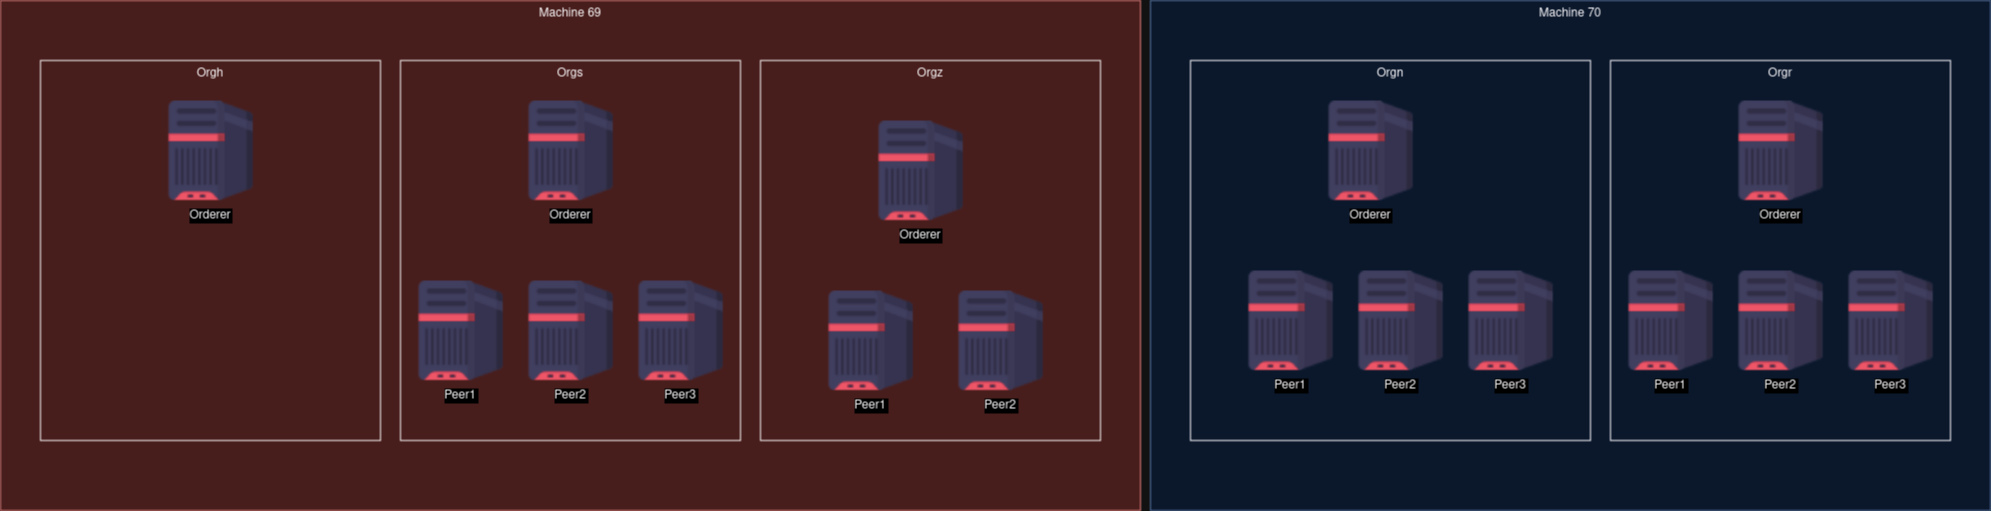
\includegraphics[width=0.5\textwidth]{assets/use-case-2/scenario3.png} % Change this to your image file
    \caption{Second use case: multiple networks scenario 3}
    \label{fig:sample-image} 
\end{figure}

In the forth scenario, in the first machine there were 4 organizations: the first had 1 orderer and 2 peers, the second 1 orderer and 3 peers, the third 1 orderer and 2 peers and the forth had 1 orderer. In the second machine, there were 3 organizations: the first had 1 orderer and 3 peers, the second had 1 orderer and 3 peers and the third had 1 orderer and 2 peers.

\begin{figure}[H]
    \centering
    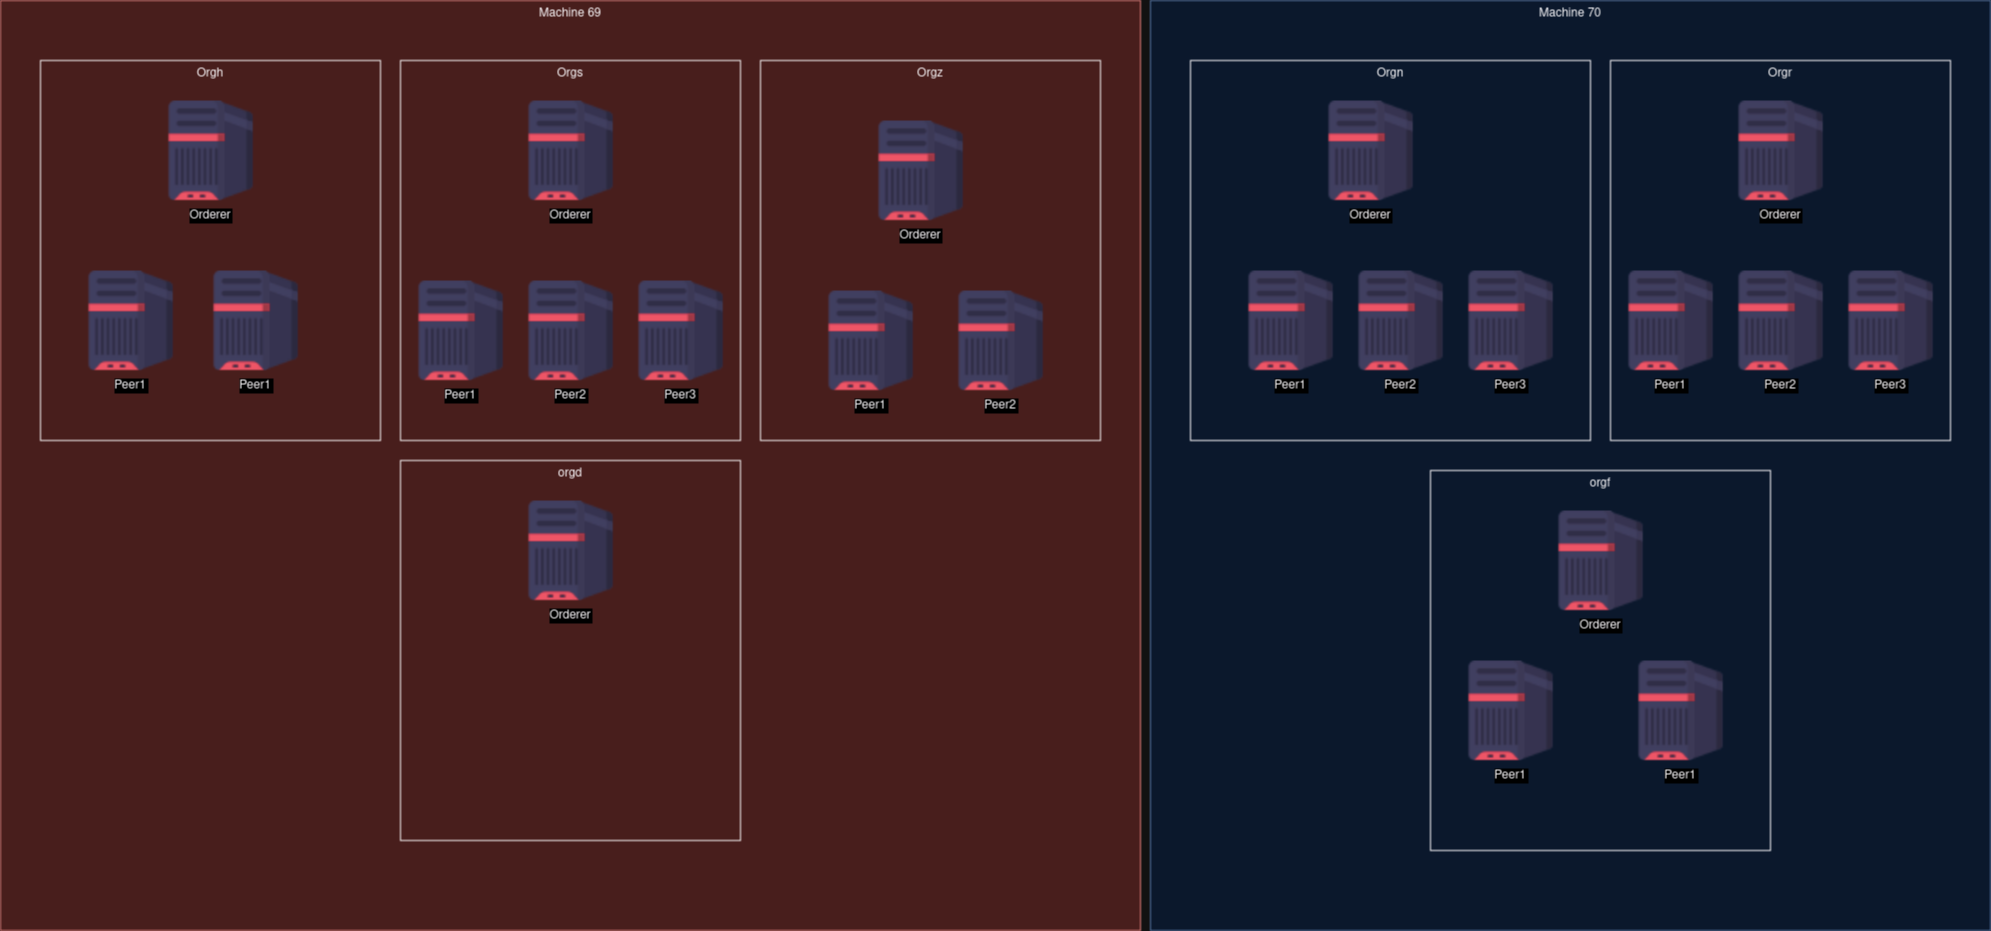
\includegraphics[width=0.5\textwidth]{assets/use-case-2/scenario4.png} % Change this to your image file
    \caption{Second use case: multiple networks scenario 4}
    \label{fig:sample-image} 
\end{figure}

In the fifth scenario, in the first machine there were 4 organizations: the first one had 1 orderer and 3 peers, the second had 1 orderer and 3 peers, the third had 1 orderer and 3 peers and the forth had 1 orderer and 3 peers. In the second machine there were 3 organizations: the first had 1 orderer and 3 peers, the second had 1 orderer and 3 peers and the third had 1 orderer and 3 peers.

\begin{figure}[H]
    \centering
    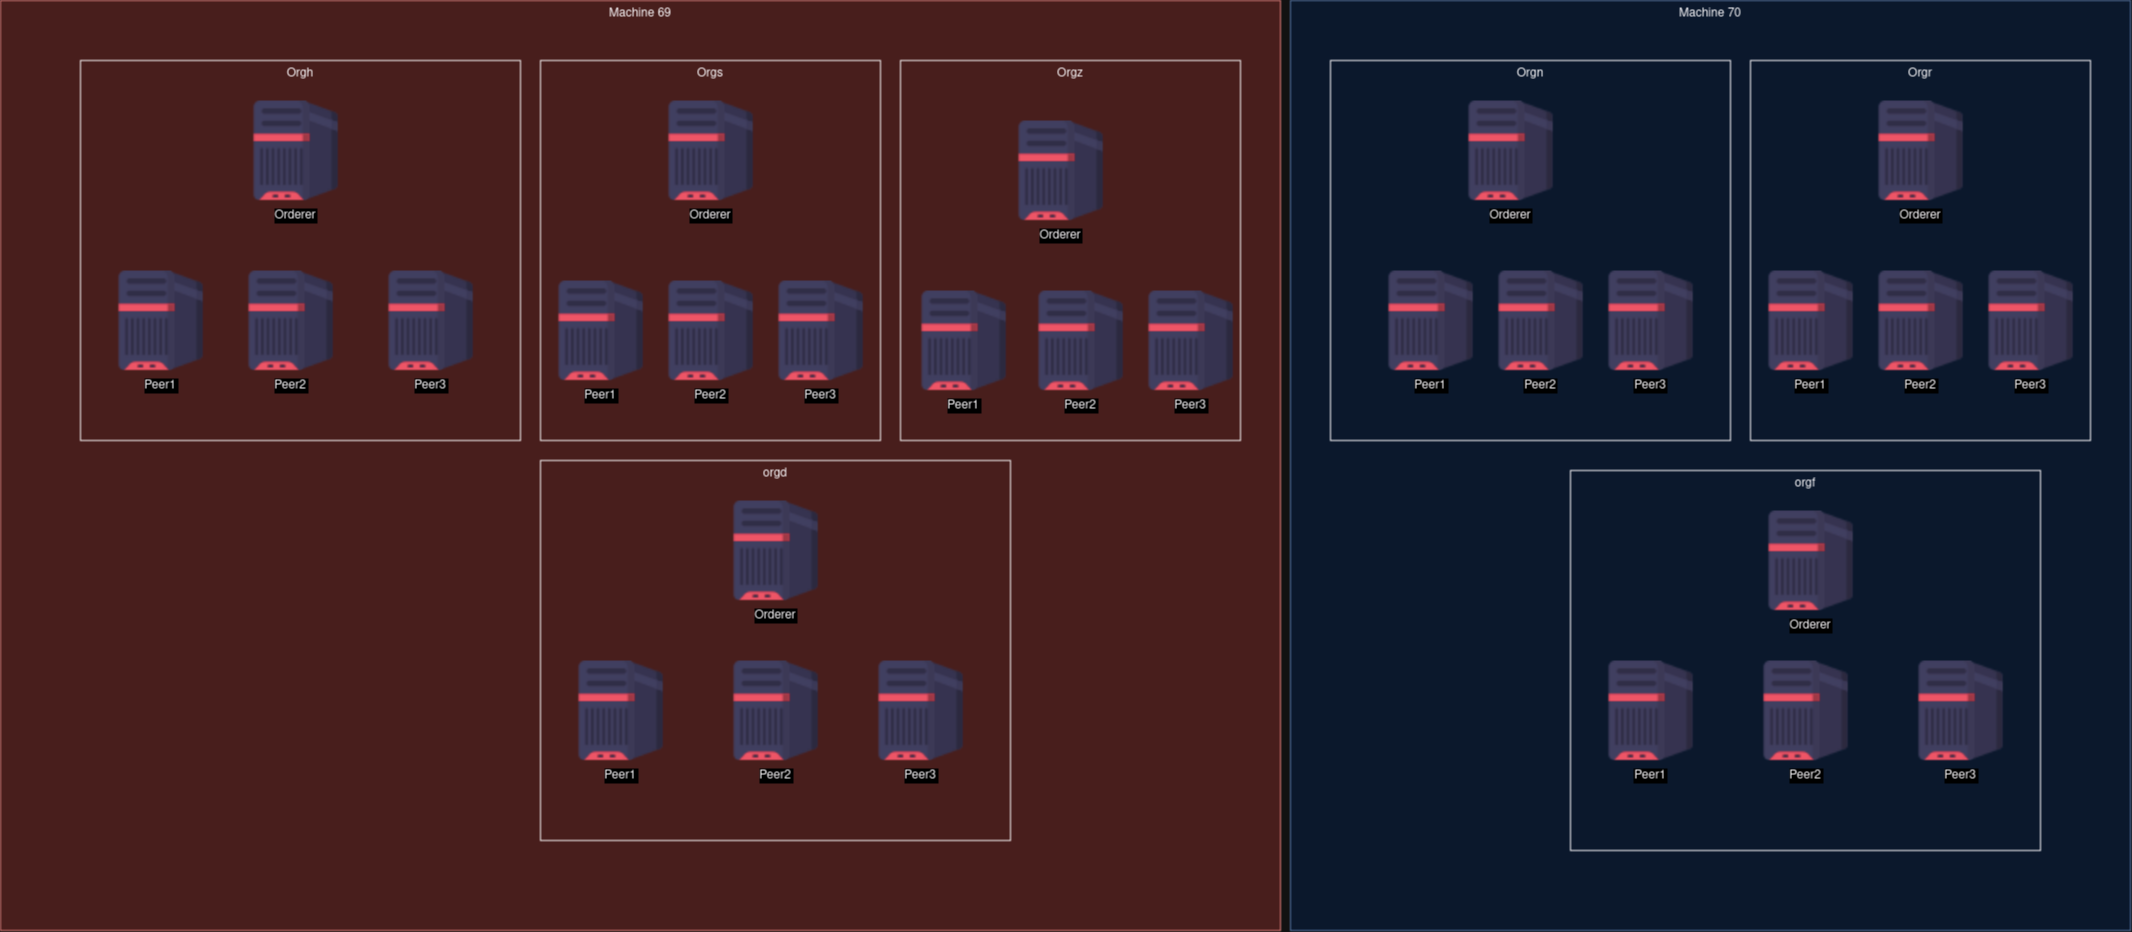
\includegraphics[width=0.5\textwidth]{assets/use-case-2/scenario5.png} % Change this to your image file
    \caption{Second use case: multiple networks scenario 5}
    \label{fig:sample-image} 
\end{figure}

Despite designing so many networks, and having in consideration that there was the removal of the kubernetes for the sake of performance unfortunately after the scenario 3 it was not possible to conduct a full benchmarking. What was noticed is that it was exceeding in remarkable ways already in terms of CPU in the scenario 3 and it needed more resources to reach the scenario 4, which makes sense since the resources were not the most powerful ones but it was interesting still to see how many components it could handle.

\paragraph{19º Phase: Benchmarking the network}\mbox{}\\
Within the realm of the 19º phase, benchmarkings were conducted. The benchmarking that was done before was refactored because of some errors in the dashboard and also because now there was the existence of a third machine which would make the tests even more interesting. By the effect of such, benchmarkins were conducted within the scope of the last network that got implemented in the hospital. In the case of the \textbf{kubernetes} implementation, there were 2 types of benchmarkings conducted: one with load balancing and another without load balancing. On another hand, in respect to the \textbf{non-kubernetes} implementation, only the normal test was considered. Because both \textbf{kubernetes} and \textbf{non-kubernetes} had the same structure of network, the data could be compared effectively. Aditionally, \textbf{jenkins} was used to automate this since it was used previously in a continuous integration perspective to come up with the side containers present in each of the components like mentioned brefore. With this, benchmarkings were totally automated both for bare metal but also for \textbf{kubernetes} which speed up even more this process and gathered all of the tests in no time.

By the effect of this, 3 architectures were under test: one architecture which only relies on \textbf{docker}, a second architecture that leverages \textbf{kubernetes} without load-balancing and a third which leverages \textbf{kubernetes} with a load-balancing.

\subparagraph{Docker} \mbox{}\\
Speaking about the considered network of \textbf{Docker}, this is composed by 3 machines with 3 different organizations. Each organization had the same amount of components like 1 peer and 1 orderer. However, since this is a network fully composed by docker containers the way the chaincode is deployed is accordinally to the default way, where each peer has it's chaincode attached to it like a side container. There are no life savers when it comes to configuring such network, which means that adding or removing components requires more work altought it has less burden when compared to kubernetes.

\begin{figure}[H]
	\centering
	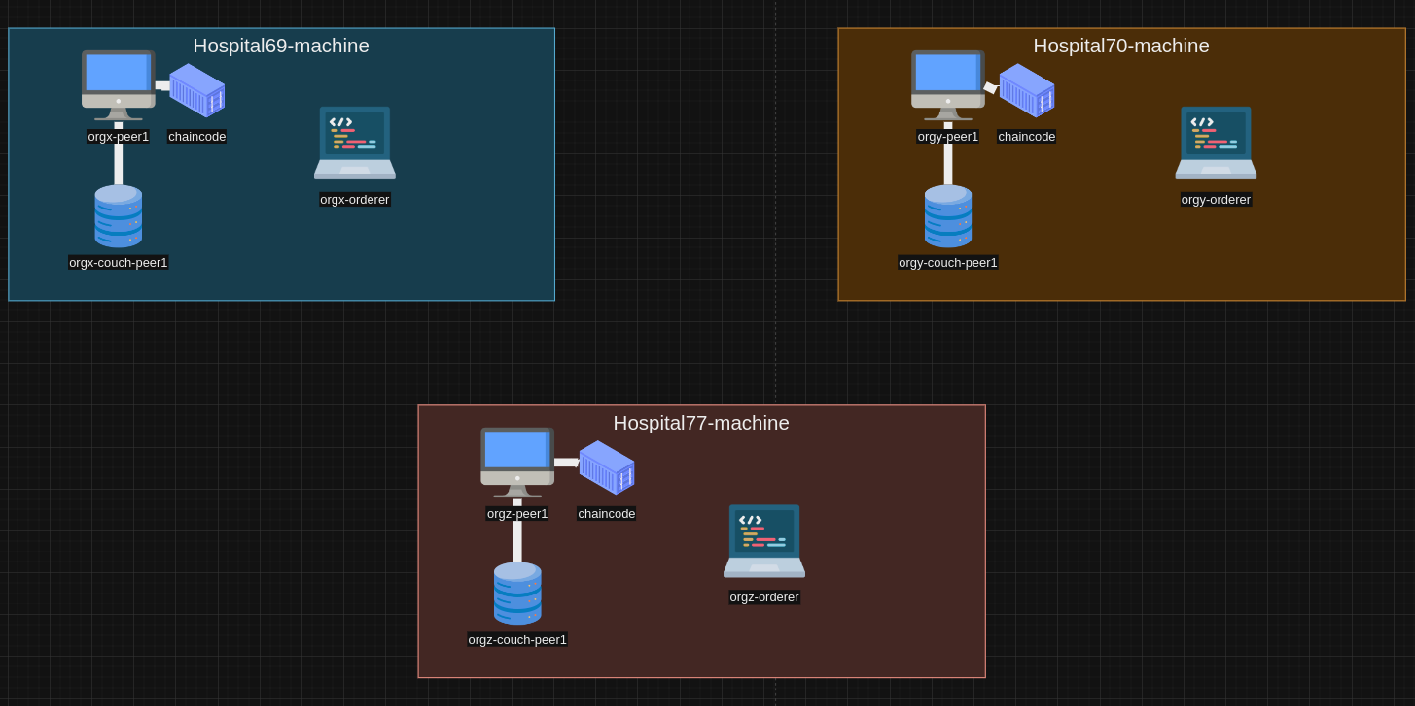
\includegraphics[width=0.5\textwidth]{assets/use-case-2/docker.png} % Change this to your image file
	\caption{Second use case: Docker only Architecture}
	\label{fig:sample-image} 
\end{figure}

\subparagraph{Kubernetes} \mbox{}\\
Reaching the \textbf{Kubernetes} considered network, there is a network with 3 different machines and 3 different peers. Each organization, like in the previous architecture, had 1 peer and 1 orderer, where the most significant changes are related to the fact that each main component had one side container attached that served as a proxy for managing configurations within the components. This approach compared to the docker one makes the management of the network easier, since there was the possibility to configure each component from the same unique point of failure (multi-client). However, this is supposed to be less performant because there is the burden of the \textbf{kubernetes}, causing a higher need of resources.

\begin{figure}[H]
	\centering
	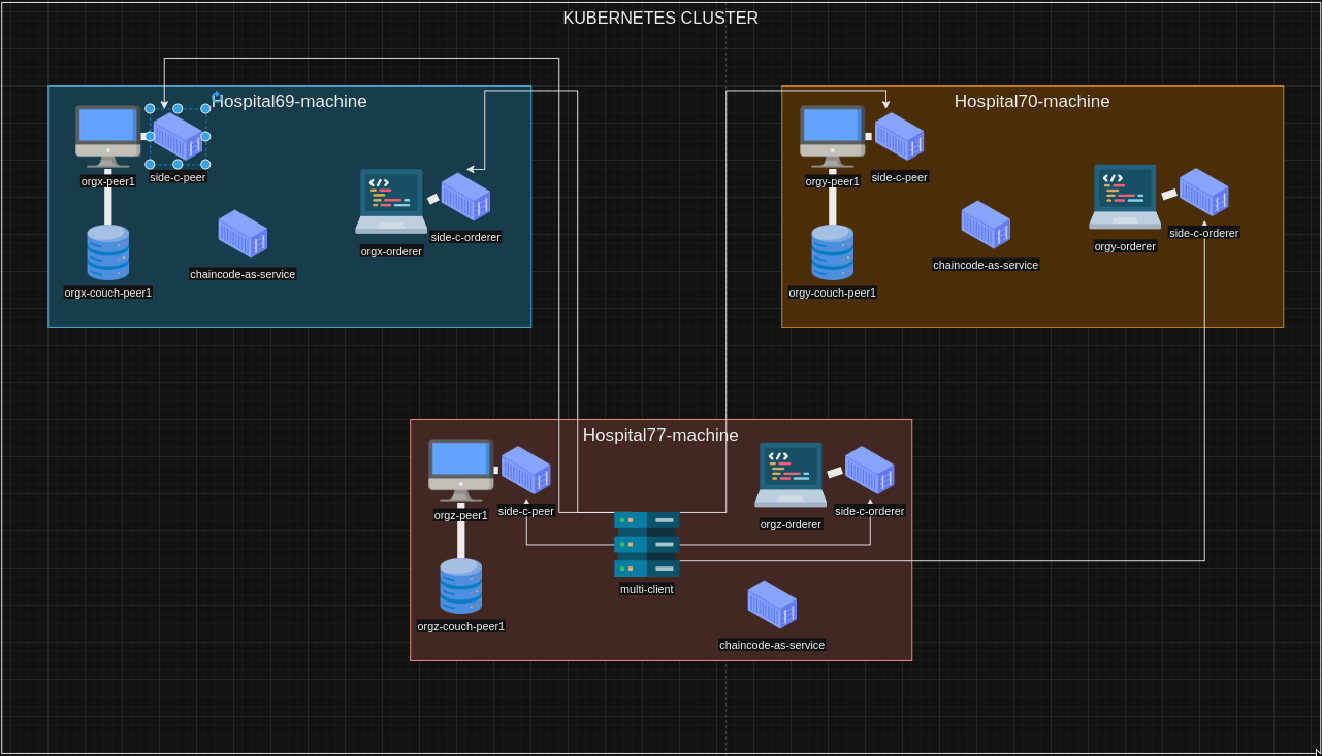
\includegraphics[width=0.5\textwidth]{assets/use-case-2/k8.png} % Change this to your image file
	\caption{Second use case: Kubernetes Archtiecture}
	\label{fig:sample-image} 
\end{figure}


\subparagraph{Kubernetes with load balancing} \mbox{}\\
When it comes to the last Architecture \textbf{Kubernetes with load balancing}, there is the same architecture as the previous \textbf{Kubernetes} one, where the difference resides in the fact that there is a addition of a load-balancer, where the load gets evenly spread among the participants of the network.
\begin{figure}[H]
	\centering
	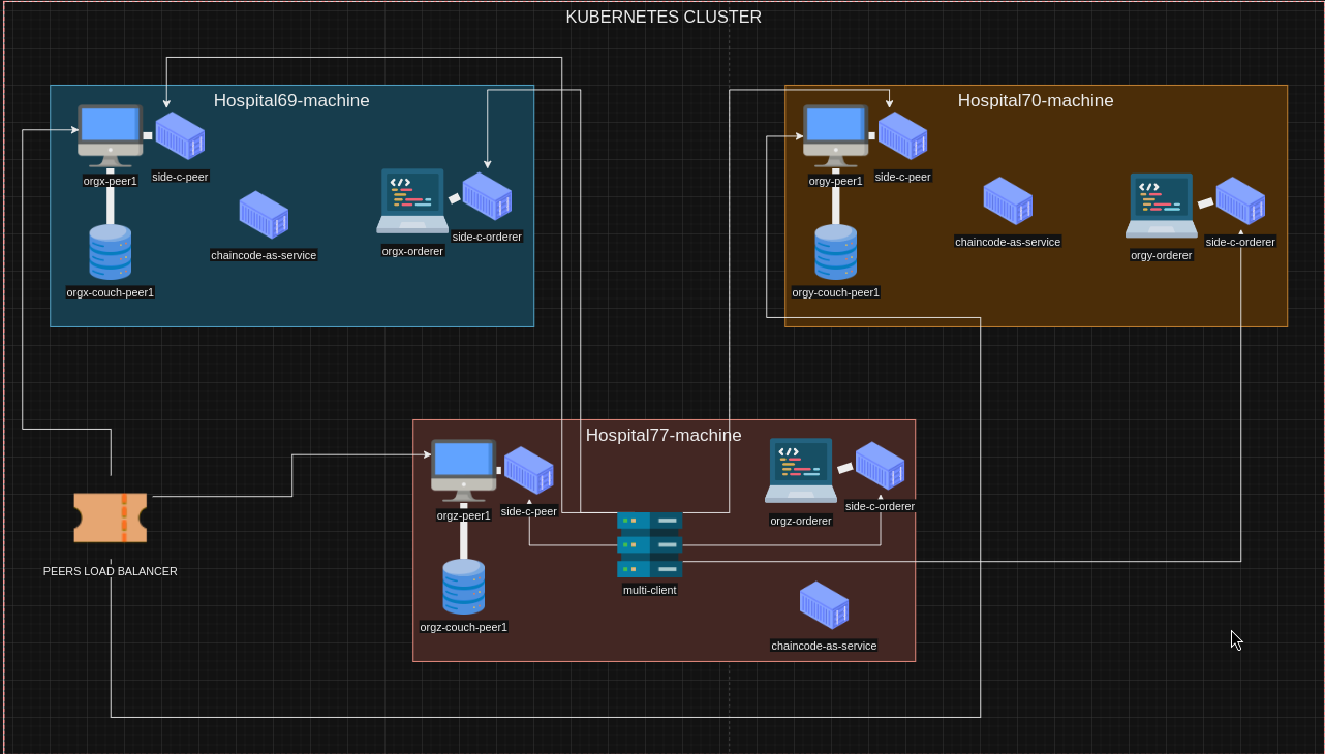
\includegraphics[width=0.5\textwidth]{assets/use-case-2/k8-lb.png} % Change this to your image file
	\caption{Second use case: Kubernetes with Load Balancer Architecture}
	\label{fig:sample-image} 
\end{figure}


\subparagraph{Evaluation} \mbox{}\\

The following image shows the results of the analysed metrics regarding the architecture that uses \textbf{Docker}, architecture 1.
In the Architecture 1 image presented below it is possible to observe the results of the metrics analysed for architecture 1. Starting the analysis with the CPU variation, this shows a sharp initial growth, followed by oscillations and a slight drop before growing again until the end where it reaches the peak with a value of 242.0.
Disk usage on this architecture starts at a low level and shows steady growth until it peaks at 0.08 GB. After this, there is a small reduction before growing again at the end of the period.
Analysing the metric, use of the ledger grows gradually over time, with some fluctuations until reaching a maximum value of 0.01 at the end of the period.
Finally, analysing the use of RAM, it shows several fluctuations. In the graph it is possible to observe specific variations, but the trend is for growth over time, reaching its maximum peak at the end of the period with a value of 1.66 GB.

\begin{figure}[H]
	\centering
	\includegraphics[width=0.5\textwidth]{assets/use-case-2/docker-evaluation.png} % Change this to your image file
	\caption{Second use case: Docker Architecture 1 Evaluation}
	\label{fig:sample-image} 
\end{figure}

The following image shows the results of the metrics analysed in both architectures. The analysis is carried out comparatively between both because they both use \textbf{Kubernetes}. They differ from each other, while architecture 2 uses \textbf{Kubernetes}, architecture 3 uses \textbf{Kubernetes} with load balancing. In this way, a comparative analysis is carried out between them.

\begin{figure}[H]
	\centering
	\includegraphics[width=0.5\textwidth]{assets/use-case-2/evaluation-of-k8-and-k8-with-lb.png} % Change this to your image file
	\caption{Second use case: Kubernetes Architecture 1 and 2 Evaluation}
	\label{fig:sample-image} 
\end{figure}

In the image related to the Architecture 1 and 2 above, it is possible to observe that architecture 2 shows a sharp increase in CPU variation, reaching higher peaks, with a maximum value of 1571.50 while architecture 3 presents a maximum peak of 1515.10. 
Analysing disk usage, both grow consistently, however, architecture 2 has a higher disk usage with a peak of 0.75 GB when compared to architecture 3 which has a peak of 0.72 GB. At the end of the analysis period, both showed a decline and subsequently stabilised.
The use of the ledger in both architectures is practically identical throughout the analysis. Both follow a similar growth trajectory, with a maximum peak of 0.01 GB.
Finally, in relation to the RAM usage metric, both grow consistently, however, architecture 3 has a slightly higher RAM usage than architecture 2 throughout the analysis period, reaching its peak at 5.63 GB.



\paragraph{20º Phase: Solutions comparison}\mbox{}\\
On this phase comparison between the previous benchmarks was done, reaching a consensus about what must be sacrificed in order to choose one over another.

\paragraph{21º Phase: Creation of extra services}\mbox{}\\
In the context of the phase 21, a set of extra services was created. This services are needed for the purpose of logging,monitoring and security. This was all done with continous integration pipelines and by leveraging technologies that enable cloud native applications inside of a \textbf{kubernetes} cluster, so the context could be the same for testing purposes.

The first service created was a own implementation of a block explorer. This proved to be very hard because, despite the gathering of data being something relatively easy to have by listening to the peer events, it was serialized in \textbf{protobuf} which means that the molding of the data should be uncovered to see in a human readable format, something that is not that easy because it is not explicitly documented and despite having the models knowing which slice of protobuf serialized data corresponds to one of the numerous existing models was something unfeasible, pretty much like a puzzle without instructions and the picture to know where which piece would fit. However, this came to a success and this extra service proved to be very useful in future iterations.

The second service created was a \textbf{quarkus} instance, conceded for making queries to the database where the block explorer was storing everything and this way serving a future client.

The third service created was a C++ web service for \textbf{prometheus} data. This is important because it is a good practise to not expose all of the \textbf{prometheus} data to the exterior, therefore the need to only expose those services that were actually in need and because the functionalities are very limited, using a high performing programming language was something that seamed better, specially because if the functionality is simple there are less concerns about eventual errors that lower level languages give, which are greater when the project complexity evolves.

The forth and final service that was created as a keycloak server, which was there to manage users. By logging in, a key was generated and could be used to authenticate a admin for him to interact with the previous mentioned services like \textbf{quarkus},\textbf{cpp} and the \textbf{graphql} single point of failure that communicates with the components side containers.

\paragraph{22º Phase: Creation of a web client application}\mbox{}\\
After the creation of extra services, something that could be used to communicate effectively with the infrastructure to supply an admin with management features is required. This management features were divided into \textbf{block explorer},\textbf{general network},\textbf{peer config} and \textbf{orderer config}.

\subparagraph{Block explorer}\mbox{}\\
This first main component was the Block Explorer, to monitor and manage network transactions. It collects and stores data through a custom implementation that captures all relevant details from the network. This data is securely stored in a database, granting easy access and analysis. 
Data is later processed by a backend architecture that makes it available to the administrative web interface.
This system allows administrators to perform a number of administrative functions over most parts of the blockchain. These include viewing the network activities by channel, the performance of the network in considerable details, and the inspection of blocks, transactions, and other related network objects. It also enables the supervision and administration of the components, as well as the channels they form part of, which are necessary for the network to operate.

\begin{figure}[H]
    \centering
    \includegraphics[width=0.5\textwidth]{assets/use-case-2/block-explorer-dashboard.png} % Change this to your image file
    \caption{Second use case: admin web client block-explorer dashboard}
    \label{fig:sample-image} 
\end{figure}

In the dashboard menu, users can access detailed metrics, including the number of blocks, transactions, nodes, chaincodes, and peers within the system. Additionally, the dashboard provides insights into the percentage of transactions categorized by organization, allowing for a clear understanding of activity distribution. A timeline-ordered block list is also available, offering a chronological view of block creation and updates. All of this information is meticulously organized by channel, enabling users to easily navigate and analyze data specific to each channel.

\begin{figure}[H]
    \centering
    \includegraphics[width=0.5\textwidth]{assets/use-case-2/block-explorer-network.png} % Change this to your image file
    \caption{Second use case: admin web client block-explorer network}
    \label{fig:sample-image} 
\end{figure}

In the network section, users can access a comprehensive list of nodes currently participating in the channel. This list is similar to the one found in the dashboard but offers more detailed information for each peer. For instance, it includes the peer's IP address, type, Membership Service Provider (MSP), the number of transactions it has processed, the number of chaincodes it supports, and its current status (whether it is active or not). As with the dashboard, all of this data is organized by channel, allowing users to focus on specific channels as needed.

\begin{figure}[H]
    \centering
    \includegraphics[width=0.5\textwidth]{assets/use-case-2/block-explorer-blocks.png} % Change this to your image file
    \caption{Second use case: admin web client block-explorer blocks}
    \label{fig:sample-image} 
\end{figure}

In the blocks section, detailed information about each block is provided, including the channel it belongs to (which is obvious since it is possible to select the channel to inspect), its data hash, the number of transactions it contains, and its size within the ledger.

\begin{figure}[H]
    \centering
    \includegraphics[width=0.5\textwidth]{assets/use-case-2/block-explorer-transactions.png} % Change this to your image file
    \caption{Second use case: admin web client block-explorer transactions}
    \label{fig:sample-image} 
\end{figure}

In the Transactions section, users can access a comprehensive overview of all transactions, each accompanied by detailed information organized by channel. This includes the creator of the transaction, the name of the channel in which the transaction occurred, the transaction ID (TX ID) for unique identification, the type of transaction performed, the name of the chaincode invoked, and the precise timestamp when the transaction was executed. This detailed breakdown, organized per channel, allows users to thoroughly analyze and track each transaction, ensuring complete transparency and traceability within the system.

\begin{figure}[H]
    \centering
    \includegraphics[width=0.5\textwidth]{assets/use-case-2/block-explorer-chaincode.png} % Change this to your image file
    \caption{Second use case: admin web client block-explorer chaincodes}
    \label{fig:sample-image} 
\end{figure}

In the Chaincodes section, users can view detailed information related to the chaincodes within a given channel, including the chaincode name, associated channel, number of transactions, and the version of each chaincode.

\begin{figure}[H]
    \centering
    \includegraphics[width=0.5\textwidth]{assets/use-case-2/block-explorer-channels.png} % Change this to your image file
    \caption{Second use case: admin web client block-explorer channels}
    \label{fig:sample-image} 
\end{figure}

In the Channels section, users can access detailed information about each channel, including the chaincode name, associated channel, the number of transactions per chaincode, the version, and the timestamp.

\subparagraph{General Network}\mbox{}\\
This part analyzes the resource utilization of the network. It provides monitoring of several performance metrics: CPU, RAM, disk usage, ledger activity, I/O operations, and network performance. Also, it presents the resources within each cluster, a graphical representation of the network's structure, and allows for an examination of their configurations and how they are organized within each component's directory.

\begin{figure}[H]
    \centering
    \includegraphics[width=0.5\textwidth]{assets/use-case-2/general-network-dashboard.png} % Change this to your image file
    \caption{Second use case: admin web client general network dashboard}
    \label{fig:sample-image} 
\end{figure}

In the “Dashboard” section it is possible to have a glance of all the network like: checking number of nodes, alive nodes, dead nodes, CPU variation\%, disk usage per machine GB, disk usage machine\%, RAM per machine GB, RAM per machine\%. Relatively to the network scheme, that's a probable future feature of changing between clusters because this is cluster-oriented.

\begin{figure}[H]
    \centering
    \includegraphics[width=0.5\textwidth]{assets/use-case-2/general-network-resources.png} % Change this to your image file
    \caption{Second use case: admin web client general network resources}
    \label{fig:sample-image} 
\end{figure}

The "Resources" section provides a list of the services residing in that cluster, each corresponding to the DNS name of that service.

\begin{figure}[H]
    \centering
    \includegraphics[width=0.5\textwidth]{assets/use-case-2/network-visualization.png} % Change this to your image file
    \caption{Second use case: admin web client general network resources}
    \label{fig:sample-image} 
\end{figure}

In the "Network Visualization" section, a cluster-oriented representation of the current components is provided. This view is cluster-oriented because it displays resources based on what exists in the cluster rather than on a specific network channel. If it were based on a network channel, the visualization could include components outside of the cluster.

\subparagraph{Peer Config}\mbox{}\\
This section deals with peer management and provides a comprehensive user interface for performing all standard peer operations, like: uploading configurations, querying, fetching and joining channels, installing, querying, aproving and committing chaincode, checking chaincode approvals, invoking chaincode for testing, and executing custom commands for more advanced operations.

\begin{figure}[H]
    \centering
    \includegraphics[width=0.5\textwidth]{assets/use-case-2/peer-config-upload-configs.png} % Change this to your image file
    \caption{Second use case: admin web client peer config upload of configurations}
    \label{fig:sample-image} 
\end{figure}

This section allows for the upload of pair definitions, as well as the chaincode package for installation. To do this, a pair is selected to proceed with this process.

\begin{figure}[H]
    \centering
    \includegraphics[width=0.5\textwidth]{assets/use-case-2/peer-config-query-channels.png} % Change this to your image file
    \caption{Second use case: admin web client peer config query of channels}
    \label{fig:sample-image} 
\end{figure}

This section makes it possible to consult the channels to which a particular peer is connected, and that is why to get to this point it is necessary to select a particular peer.

\begin{figure}[H]
    \centering
    \includegraphics[width=0.5\textwidth]{assets/use-case-2/peer-config-fetch-channel.png} % Change this to your image file
    \caption{Second use case: admin web client peer config fetch a channel}
    \label{fig:sample-image} 
\end{figure}

In this section, searching for an order channel is possible. To achieve this, the channel name, TLS CA file path, certificate file path, key file path, and IP address of the requestor from which it fetches the channel are provided.

\begin{figure}[H]
    \centering
    \includegraphics[width=0.5\textwidth]{assets/use-case-2/peer-config-join-channel.png} % Change this to your image file
    \caption{Second use case: admin web client peer config join channel}
    \label{fig:sample-image} 
\end{figure}

In the "Join Channel" section, joining a channel is enabled by selecting the correct searched channel on a given peer.

\begin{figure}[H]
    \centering
    \includegraphics[width=0.5\textwidth]{assets/use-case-2/peer-config-install-chaincode.png} % Change this to your image file
    \caption{Second use case: admin web client peer config install chaincode}
    \label{fig:sample-image} 
\end{figure}

In this "Install Chaincode" section, access to files uploaded from the "Upload Configs" section is provided, making it easy to select the desired chaincode.tar.gz file for installation.

\begin{figure}[H]
    \centering
    \includegraphics[width=0.5\textwidth]{assets/use-case-2/peer-config-query-chaincode.png} % Change this to your image file
    \caption{Second use case: admin web client peer config query chaincodes}
    \label{fig:sample-image} 
\end{figure}

The "Consult Installed Chaincode" section provides access to the chaincodes that are already installed.

\begin{figure}[H]
    \centering
    \includegraphics[width=0.5\textwidth]{assets/use-case-2/peer-config-approve-chaincode.png} % Change this to your image file
    \caption{Second use case: admin web client peer config approve chaincode}
    \label{fig:sample-image} 
\end{figure}

The "Approve Chaincode" section provides all the information needed to approve a chaincode, including the channel name, chaincode name, chaincode version, package ID, sequence, TLS CA certificate path, CA certificate path, private key path, and orderer IP address.

\begin{figure}[H]
    \centering
    \includegraphics[width=0.5\textwidth]{assets/use-case-2/peer-config-query-chaincode-approvals.png} % Change this to your image file
    \caption{Second use case: admin web client peer config query chaincode approvals}
    \label{fig:sample-image} 
\end{figure}

The "Querying chaincode approvals" section provides a form with all the fields needed to query chaincode approvals, including the channel name, chaincode name, version, sequence, TLS CA certificate path, CA certificate path, and private key path.

\begin{figure}[H]
    \centering
    \includegraphics[width=0.5\textwidth]{assets/use-case-2/peer-config-commit-chaincode.png} % Change this to your image file
    \caption{Second use case: admin web client peer config commit chaincode}
    \label{fig:sample-image} 
\end{figure}

The "Commit Chaincode" section provides all the fields required to commit a chaincode to a given peer and channel, including the orderer IP, chaincode name, channel name, chaincode version, required peer signatures, chaincode sequence, and the TLS CA file for connecting to the peer.

\begin{figure}[H]
    \centering
    \includegraphics[width=0.5\textwidth]{assets/use-case-2/peer-config-invoke-chaincode.png} % Change this to your image file
    \caption{Second use case: admin web client peer config invoke chaincode}
    \label{fig:sample-image} 
\end{figure}

In the "Invoke Chaincode" section, I have all the necessary information to invoke a chaincode, including the orderer IP, channel name, chaincode name, TLS CA certificate path, certificate path, private key path, function name, and arguments separated by commas.

\begin{figure}[H]
    \centering
    \includegraphics[width=0.5\textwidth]{assets/use-case-2/peer-config-custom-commands.png} % Change this to your image file
    \caption{Second use case: admin web client peer config custom commands}
    \label{fig:sample-image} 
\end{figure}

In the "Custom Commands" section, I have all the necessary tools to create a custom command with a peer, which can be valuable in unexpected situations.

\subparagraph{Orderer Config}\mbox{}\\
This section focuses on the management of the orderer and provides a comprehensive set of tools for efficiently handling all regular duties. Users can create new channels, join existing ones, and execute custom commands for more complex configurations.

\begin{figure}[H]
    \centering
    \includegraphics[width=0.5\textwidth]{assets/use-case-2/orderer-config-creating-channel.png} % Change this to your image file
    \caption{Second use case: admin web client orderer config creating a channel}
    \label{fig:sample-image} 
\end{figure}

This section is designed to create a channel for a selected orderer. To do this, an order is selected, a channel configuration file (configtx.yaml) is attached, the channel is named, and finally the request is sent.

\begin{figure}[H]
    \centering
    \includegraphics[width=0.5\textwidth]{assets/use-case-2/orderer-config-join-channel.png} % Change this to your image file
    \caption{Second use case: admin web client orderer config join a channel}
    \label{fig:sample-image} 
\end{figure}

The "Join Channel" section is designed to facilitate joining a channel. Here, all necessary components are displayed. These include the channel junction file, channel name, requestor IP, TLS CA path, client certificate, and client private key.

\begin{figure}[H]
    \centering
    \includegraphics[width=0.5\textwidth]{assets/use-case-2/orderer-config-query-channels.png} % Change this to your image file
    \caption{Second use case: admin web client orderer config query channels}
    \label{fig:sample-image} 
\end{figure}

This section is for querying the channels associated with a given order. To perform the query, the request IP, TLS CA path, client key path, and client certificate path must be provided.

\begin{figure}[H]
    \centering
    \includegraphics[width=0.5\textwidth]{assets/use-case-2/orderer-config-custom-commands.png} % Change this to your image file
    \caption{Second use case: admin web client orderer config custom commands}
    \label{fig:sample-image} 
\end{figure}

This is the custom commands section. Custom commands are executed in the order component if there is a need for a personalized interaction with it.

\subparagraph{Final Architecture}\mbox{}\\
After having the web client application, it could be said that the final architecture was achieved. There may be some improvements in the future but the most of it was already accomplished.

In this final architecture, it was implemented with the same setup as the one verified in the Kubernetes with load balancer. Here, the architecture is presented with additional components that are essential to a production environment. With this in mind, besides the core components, there are also: prometheus (for fetching the data from all the cadvisors and also components of the network), cadvisor (measures collector for prometheus), cpp-rest-service (to wrap the data from prometheus and serve it to the admin web server; it is a good practice to not expose entirely the prometheus API), keycloak (for users management), blockexplorerlistener (a developed implementation of a blockexplorer listener to grab the data from events and store it on a database), postgresql-blockexplorer (database for the blockexplorer listener), and quarkus rest for serving this blockexplorer data to the admin web server. Note that the multi-client now serves the admin web server.

\begin{figure}[H]
    \centering
    \includegraphics[width=0.5\textwidth]{assets/use-case-2/final-arch.png} % Change this to your image file
    \caption{Second use case: final architecture}
    \label{fig:sample-image} 
\end{figure}

\subsubsection{Discussion}

Throughout this section, the different architectures will be
discussed accordinally to previous testing results, considering them in terms of scalability and sustainability. Also, a \textbf{SWOT} diagram will be presented, to understand the strengths,weaknesses,opportunities and respective threats.

\paragraph{Architectures discussion}\mbox{}\\

The following table represents the main sides to take into accordance when it comes to choose between the kubernetes and the docker architecture.

\begin{longtable}{| c | c | c |}
	\hline
	 \textbf{Characteristic} & \textbf{Docker} & \textbf{Kubernetes} \\ \hline
	
	More performance for smaller environments & X & \\ \hline
	
    Less abstract and easier to learn & X & \\ \hline
	
	Incorporated load balancer &  & X \\ \hline
	
	Resource management &  & X \\ \hline
	
	Robust API for managing resources &  & X \\ \hline
	
	High availability &  & X \\ \hline
	
	Built-in mechanism for horizontal scaling &  & X \\ \hline
	
	Higher resource overhead &  & X \\ \hline
	
	\caption{Second use case: Characteristics comparasion between docker and kubernetes} \label{tab:activity_schedule} 
\end{longtable}

While \textbf{Kubernetes} does come with a steeper learning
curve and a higher resource overhead, these complexities are
justified in larger, more complex environments. In this case,
The smaller environment favors Docker for its performance.
and ease of use. However, as the project expands and the
environment scales, \textbf{Kubernetes} will likely become the more
beneficial option due to its advanced features and ability to
handle larger workloads.
Regarding the comparison between Architecture 2 and 3,
even though the implementation of a load balancer had only
residual benefits in some of the metrics and that its
Implementation may introduce complexity to the
development of the network, it provides several advantages
that, in the long term, can be very beneficial. It can ensure
better scalability, reliability, resource allocation, and
performance, contributing for the solution sustainability over
time.
In summary, \textbf{Docker} has proven to be the more
performant solution for the current, smaller environment.
Yet, this project relies on \textbf{Kubernetes} for specific aspects,
such as the UI tool, due to its powerful API and management
capabilities.  As growth is anticipated, the robust
management and high availability offered by Kubernetes by
Deploying a load balancer will become increasingly valuable.
making it the preferred choice in larger, more complex
deployments. 

\paragraph{SWOT analysis}\mbox{}\\

The following figure dictates a \textbf{SWOT} analysis for the second use case project.

\begin{figure}[H]
	\centering
	\includegraphics[width=0.5\linewidth]{assets/use-case-2/SWOT-use-case-2}
	\caption{Use case 2: SWOT analysis}
	\label{fig:swot-use-case-2}
\end{figure}

\subsubsection{Conclusion}
To summarize, in terms of infrastructure architectures, three implementations were developed during the project: one using \textbf{Docker}, the other using Kubernetes, and a third one using \textbf{Kubernetes} alongside a load balancer. This implementation evolved as we developed further in time, aiming to firstly create the most basic network (docker), secondly to present a more robust architecture that could also be used to manage better an infrastructure that could evolve in number of components with time (kubernetes), and lastly to an infrastructure where we could balance traffic within the same channel contained in a certain number of components (kubernetes with load balancing). Docker is suitable for small businesses due to its greater simplicity and ease of use, although there is more overhead around setting how components must communicate, while Kubernetes is better for treating components as simple resources designed for larger, more complex environments, more scalable, more incremental, and easier to maintain architectures. We also benefit from features provided by the Kubernetes API that we can use to obtain information about concrete resources that we can use to create analysis tools like the ones mentioned in our project. With \textbf{Kubernetes}, regardless of the number of components we have, we will be able to use this analysis tool without further configurations than the resource itself. The \textbf{Kubernetes} with load balancer (K8 with LB) approach was chosen. This makes sense because of all of the characteristics mentioned so far that are very suited for an infrastructure for the healthcare industry—a sector that demands a large, resilient infrastructure and advanced features to manage and monitor the network for its administrators, aligning with our primary goal.

Speaking about the platform itself, the system developed provides a robust and comprehensive solution for monitoring and managing the \textbf{HLF} network. This is only possible due to the selected solution. The system guarantees continuous access and analysis through its design architecture, where various critical statistics are consolidated. This system not only replicates but also improves on the functionality of previous solutions, allowing administrators to perform a wide range of tasks with greater efficiency and precision all in one single place, reducing errors as common network tasks are successfully automated and monitoring is provided. More concretely, the system provides more than a basic network management. It offers information about resource utilization, peer management, and orderer operations. It also provides a user-friendly interface to easily handle complex tasks such as monitoring network activity, managing resources, or adjusting settings. This is a solution that offers everything that an administrator needs to control its network.

\subsubsection{Future Work}
Since blockchain networks are not a basic matter and managing multiple components in that realm scalates to even more complex situations, future work regarding what has been covered so far is more than needed. The work that remains to be done ranges from observing further details about the infrastructure chosen architecture and processes refining to improving existing solutions that have been constructed so far. There is no perfect system, and thinking forward to collate possible issues is more than a primary key. However, additions to the current implementation are out of question since the more is introduced, the more features must be supported, thereby quality can be sacrificed.

By the effect of such, in this section, the most critical future work in mind will be covered and explained in a brief way.

\paragraph{Horizontal Scaling in a HyperLedger fabric network}\mbox{}\\

\textbf{Horizontal scaling}, or scale-out, is a critical optimization of the system to manage more workload—notably within containerized environments—into one node, while horizontal scaling will increase the number of nodes to share a load over more than one machine.
This means that in the case of \textbf{Hyperledger Fabric} (HLF), which is a commonly used distributed ledger platform for blockchain-based solutions, there is a potential application of horizontal scaling. It would be quite interesting, to say the least. In the case of \textbf{Hyperledger Fabric} (HLF), since a network often involves the co-existence of multiple organizations, which are usually referred to as consortiums, the potential key issue of effective performance optimization may lie in the ability to scale horizontally when the size and complexity of this kind of network grows. Horizontal scaling will allow the number of instances in the system to bend with real-time traffic demands, or surges in computational work—things that normally accompany every organization in an HLF network. Every organization within an HLF network operates its own set of peers including services for ordering and many other components.
In this regard, we will predict for subsequent work how much horizontal scaling can be done with an HLF network. We will look especially at when it can be pushed forward—when no diminishing returns from the system's architecture meet a bottleneck. This will comprise the evaluation of different factors like latency, throughput, and resource usage under different scaling scenarios. We also want to verify if the application of horizontal scaling in such networks offers real advantages for large consortiums, mainly those operating with a high volume of transactions or in need of high fault tolerance.
This is significant potential for research, as it could bring insight that is useful to organizations running large-scale \textbf{HLF} networks. With this, architectural teams would then have the knowledge of whether horizontal scaling really yields measurable improvement in performance and resilience that is satisfying to their operational needs. Finally, findings emerging from this work may help consortiums understand the trade-offs involved and make a decision on whether horizontal scaling could really be a feasible and beneficial approach for the considered blockchain projects.


\paragraph{Automating Network Component Generation}\mbox{}\\
This will focus on automating the generation of network components, such as peers and orderers, directly in a user interface (UI). This automation will be possible by using scripts and a standard template to the creation process, reducing the need for manual configuration which results in a reducing of errors. By integrating this directly in the the UI, we can significantly improve operational efficiency by enabling rapid deployment and management of HLF components. This approach will allow network administrators to create new components with ease, which will give them more time to plan how exactly they want their network to be because creating it by themselves creates a huge overhead due to the number of configurations that can result in unexpected behavior, which may cause a very huge loss of time.

\paragraph{Creating Recovery Plans for HLF Components}\mbox{}\\
Because the \textbf{HLF} is a complex infrastructure, developing recovery plans for components is of much importance. With this in mind, it is planned to actually  create a set of detailed plans for given situations that outline the steps necessary to quickly identify, contain, and recover from failures in these components. These recovery plans will be essential to know exactly what to do when some unknown behavior happens, which is something that we should give special attention to due to the importance of the probable use case. By implementing these recovery strategies, organizations can feel confident to use our solution for their \textbf{HLF} networks and know for sure that the system remains resilient to a vast number of situations, preserving data integrity and service continuity. In case some new case occurs, we have also plans to create a community that communicates faced challenges, that later one could be added to this recovery plans because this work must be continuous.

\paragraph{Improving Documentation Practices}\mbox{}\\
Documentation often lacks clarity and accessibility, which can lead to misunderstandings and inefficiencies while working with the given product. Because we have our own documentation for this project, it is important to refactor it in order to create well-formatted documentation that is easy to use and clearly explains how to complete certain tasks that may be required depending on the objective of the administrator. Improving the documentation is something that we see as very important, as it will be the basis for current and future administrators and programmers to take advantage of the created features in our project, making it easier to work with. It also helps with onboarding new team members and ensuring consistent practices across the organization. The point of access to our documentation is still under work, but it is expected to be available in our UI.


\paragraph{Improving the current UI}\mbox{}\\
Despite being very composed, our current UI must be even more improved. There are features to be added and others that must have further modification, as for now it is still in a beta version. With this in mind, we want to: Add a menu for documentation, which we already discussed in the section before, and develop a mechanism that allows administrators to select and manage multiple clusters simultaneously in order to address the increasing complexity of network infrastructures. This multi-cluster management capability will be a good ally for managing multiple clusters, which may be a big ally for bigger organizations, improving scalability and reducing administrative burden. In addition to what was previously mentioned, a new menu option will be introduced precisely to provide a tree model view of the component structure. This feature is meant to understand the current position of given artifacts needed for certain operations within the network (certificates, config blocks, etc.).Finally, the development of a geopositioning map that aims to display the physical location of network components. This feature will allow administrators to view the geographic distribution of components, which can be something valuable for physical interaction with components of the cluster (like a node, for example). Although not as relevant as the other ideas discussed before, it remains a very good feature for this project.

\paragraph{Developing Prototypes for Enhanced Security Protocols}\mbox{}\\
Because security is so important, especially in the context of service authentication within the network, there is a need to strengthen the procedures to this effect. With this in mind, there is future work that must involve the development of prototypes for security protocols. The idea is to implement optional extra steps for authentication that secure even more our platform. This is what will enable those services that collect block explorer data, manage peer connections, and manipulate Prometheus data servers. These new protocols will focus on strengthening the security of those services, ensuring that they are protected against unauthorized access and potential threats. There are ideas that got discussed already about this matter, like, for example, creating a structure that does not allow access if one of the steps gets compromised. Also something that will evolve more and more with the time.

\paragraph{Gathering Regulatory Information on Private Ledgers}\mbox{}\\
As private ledgers are being developed, remaining informed about the regulatory landscape will be very crucial. It therefore follows that there is future work related to collecting and analyzing information about regulations related to private ledgers. Such regulations make it easier to shape the network architecture for it to meet the legal impositions that exist around different countries or even use common standards to have broad acceptance of the platform. This work is also incremental, especially in view of the emergent nature of the matter discussed, where more and more standards come into play.